\documentclass[12pt,a4paper]{article}
\usepackage[utf8]{inputenc}
\usepackage[brazil]{babel}
\usepackage{graphicx}
\usepackage{hyperref}
\usepackage{abnt-alf}
\usepackage[top=3cm,bottom=2cm,left=3cm,right=2cm]{geometry}
\usepackage{indentfirst}
\usepackage{longtable}
\usepackage{lscape}
\usepackage{vaucanson-g}
\usepackage{amsmath}
\usepackage{amsfonts}
\usepackage{algorithmic}
\usepackage{algorithm}
\usepackage{float}

% CAPA
\pagestyle{empty}
\begin{document}
\begin{center}
\large  \textbf{UNIVERSIDADE PRESBITERIANA MACKENZIE}
\large  \textbf{PROGRAMA DE PÓS-GRADUAÇÃO EM}\\
\large  \textbf{ENGENHARIA ELÉTRICA}\\
\vskip 2.0cm
\textbf{\large Wander Lairson Costa}\\
\vskip 3.5cm
\setlength{\baselineskip}{1.5\baselineskip}
\textbf{\large Complexidade de linguagens regulares de autômatos celulares elementares através da análise das matrizes de adjacências dos autômatos finitos intermediários}\\
\vskip 4.0cm
\end{center}
\hfill{\vbox{\hsize=8.5cm\noindent\strut
Dissertação de Mestrado apresentada ao\break
Programa de Pós-Graduação em Engenharia\break
Elétrica, como parte das Exigências para\break
Obtenção do Grau de Mestre em Engenharia\break
Elétrica, na Área de Concentração em\break
Engenharia da Computação.}\\
\strut}
\vskip 2.0cm
\textbf{\normalsize Orientador: Pedro Paulo Balbi de Oliveira}\\
\vskip 2.0cm
\begin{center}
São Paulo\\
ANO 2011\\
\end{center}

% RESUMO
\newpage
\thispagestyle{plain}
\pagenumbering{roman}
\begin{center}
\large  
\textbf{RESUMO}
\end{center}
\renewcommand{\baselinestretch}{0.6666666}
Autômatos celulares são sistemas discretos no tempo e no espaço que possuem
comportamento local simples e determinísticos, mas cujo comportamento global
pode ser extremamente complexo. O conjunto de possíveis configuração globais 
em um passo de tempo $t$ para um autômato celular pode ser descrito por um
linguagem regular. Este trabalho propõe o estudo da complexidade da
evolução dos autômatos celulares por meio de matrizes de adjacências. É
demonstrado que a notação clássica de matrizes de adjacências é
insuficiente para completamente descrever os semi-autômatos dos
autômatos celulares, e uma nova representação é proposta. Conclui-se que
esta nova representação facilita a análise da complexidade de autômatos
celulares e a detecção de padrões de crescimento. Sobretudo, é
mostrado que é possível obter um algoritmo para geração do semi-autômato de
tempo $t$ a partir da análise das sucessivas matrizes de adjacências.
\\[0.5cm]
\begin{flushleft}
{\bf Palavras-chave:} {\it autômatos celulares, comportamento limite, linguagens regulares.}
\end{flushleft}

% SUMÁRIO
\newpage
\thispagestyle{empty}
\tableofcontents

% DESENVOLVIMENTO
\newpage
\pagestyle{plain}
\pagenumbering{arabic}
\renewcommand{\baselinestretch}{1.5} 
\normalsize

\newcommand{\citecustom}[1]{[\citeauthoronline{#1}, \citeyear{#1}]}

\section{Introdução}

Autômatos celulares são sistemas discretos que apresentam um comportamento
local extremamente simples, mas cujo comportamento global pode ser tão
complexo quanto uma máquina de Turing \citecustom{wolfram1984a}. Ele
é caracterizado por um reticulado de células cujos estados posteriores
dependem dos estados anteriores de si próprias e de suas vizinhas.
Este tipo de comportamento, que é localmente simples mas globalmente
complexo da origem à chamada \textit{computação emergente}. 
Autômatos celulares são utilizados na modelagem de diversos sistemas
físicos e naturais.

A vizinhança das células de um autômato celular por ser definida por
um raio que tem seu centro na célula em questão. Um autômato celular
elementar possui um raio igual a 1 e um conjunto de estados $\{0,1\}$.
Este trabalho estuda um subconjunto dos autômatos celulares elementares.

O comportamento limite de autômatos celulares pode ser descrito por meio
de linguagens formais. Uma linguagem formal é um conjunto de cadeias ou
palavras formadas a partir de um alfabeto da linguagem
\citecustom{lewis2008}. A classe mais simples de linguagens formais é
a das linguagens regulares, que pode ser gerada por uma gramática regular ou
pelas chamadas expressões regulares. Uma linguagem regular pode ser
reconhecida por um autômato finito, que é um tipo de autômato que
não possui memória. As linguagens regulares são o tipo mais simples
de linguagens na hierarquia de Chomsky.

O conjunto de todas as configurações globais de um autômato celular
elementar em um dado momento no tempo discreto pode ser descrito por
uma linguagem regular e, consequentemente, um autômato finito
\citecustom{wolfram1984}. \citeonline{trafaniuc2004} e \citeonline{miki2006}
estudaram, em seus respectivos trabalhos, a complexidade de autômatos
celulares elementares por meio da análise da evolução dos sucessivos
autômatos celulares para diferentes instantes de tempo. Este trabalho
tem o objetivo de dar prosseguimento a este estudo, utilizando a abordagem
de representação dos autômatos finitos por meio de matrizes de adjacências.
Sobretudo, este trabalho objetiva encontrar um meio para derivar um
algoritmo para obtenção do autômato finito de tempo $t$ de uma regra
do espaço elementar a partir do autômato de tempo $t-1$.

O Capítulo \ref{sec:refteo} apresenta um referencial teórico sobre 
os autômatos celulares, linguagens formais e comportamento limite.
Adicionalmente, apresenta um resumo do trabalho feito por
\citecustom{mikietal2011}.

O Capítulo \ref{sec:desenv} descreve a proposta deste trabalho. A obtenção do
semi-autômato de tempo $t$ pode ser obtido por meio de uma nova notação de 
matrizes de adjacências isomórfica em relação ao respectivo semi-autômato.

O Capílulo \ref{sec:conclude} conclui o trabalho.

\section{Autômatos Celulares}\label{sec:refteo}

É comum na natureza encontrar sistemas cujo comportamento global é extremamente
complexo, ainda que as partes que formam tais sistemas sejam simples. A
complexidade é gerada pelo efeito cooperativo de componentes com regras locais
simples. Muito foi descoberto sobre a natureza dos componentes em sistemas físicos
e biológicos, mas pouco é conhecido sobre os mecanismos pelos quais tais componentes
agem cooperativamente para gerar o comportamento global observado \citecustom{wolfram1984a}.

Autômatos Celulares podem ser vistos como uma classe de sistemas dinâmicos de dimensão
infinita cujo tempo, espaço e estado são todos discretos e os estados de cada célula
podem ser obtidos de uma conjunto finito de estados possíveis \citecustom{zhisong2001}. 

Autômatos celulares são, fundamentalmente, as representações matemáticas mais simples
de uma classe muito maior de sistemas complexos (onde \textit{sistema complexo} significa
qualquer sistema dinâmico que consiste de mais do que algumas poucas - tipicamente
não lineares - partes que se interagem). Assim, autômatos celulares têm se provado
serem idealizações extremamente úteis do comportamento dinâmico de muitos sistemas
complexos reais, incluindo fluídos físicos, redes neurais, sistemas dinâmicos
moleculares, ecologias naturais, comando militar e redes de controle, economia, entre
outros. Por causa de sua simplicidade subjacente, autômatos celulares são máquinas
conceituais poderosas com as quais se estuda padrões generalizados de formação. Eles
já forneceram ideias cruciais sobre auto organização de reações químicas, sistemas de
difusão, crescimento de cristais, formação de padrões de conchas e fenômenos em fluxo
de tráfego veicular, para citar alguns exemplos. Em um lado mais prático, autômatos
celulares fornecem a base de algoritmos de criptografia extremamente poderosos. Existe
até mesmo algumas sérias especulações de que autômatos celulares possam fornecer
a espinha dorsal de uma radicalmente discreta física fundamental \citecustom{ilachinski2002}.

Os primeiros estudos de autômatos celulares por John von Neumann no final da década de
40 tinha como meta desenvolver sistemas computacionais auto replicantes que também fossem
computacionalmente universais. von Neumann queria investigar dispositivos sintéticos de
computação análogos ao cérebro humano no qual a memória e as unidades de processamento
não são separadas uma da outra, e que fossem massivamente paralelos e capazes de se
auto reparar e reproduzir dado o material base necessário. Segundo sugestões de
Stanislaw Ulam, von Neumann visualizou um universo discreto consistindo de uma grade
bidimensional de máquinas de estado finito, chamadas células, interconectadas
internamente umas com as outras \citecustom{kari2005}. O autômato originalmente descrito por
von Neumann é um vetor uniforme infinito bidimensional de células, onde cada célula é
conectada pelos seus quatro vizinhos ortogonais. As primeiras estruturas estudadas eram
em sua maioria de uma ou duas dimensões, apesar de dimensões maiores também terem sido
consideradas \citecustom{sarkar2000}.

Dois tópicos imediatos surgiram a partir do trabalho de von Neumann. O primeiro, em
sua maior parte na década de 60, era uma discussão sobre a construção de autômatos
auto replicantes. O segundo foi uma tentativa de capturar mais da essência de
auto replicância por meio de estudos matemáticos de propriedades detalhadas de
autômatos celulares. Durante o curso da década de 60 foram encontradas construções
mais simples de autômatos celulares capazes de auto replicância e computação
universal. No início da década de 60 foram notadas algumas características gerais
incrivelmente simples de autômatos celulares que acreditava-se serem relevantes para
auto replicância - e foram estudadas com um formalismo técnico mais elaborado. Existiram
também várias construções de autômatos celulares cujo comportamento mostraram
características particularmente simples talvez relevantes para auto replicância
\citecustom{wolfram2002}.

A década de 80 é um período importante na história dos autômatos celulares,
largamente devido ao trabalho executado por Stephen Wolfram. A natureza de suas questões
representa uma mudança de paradigma na pesquisa com autômatos celulares. Wolfram conduziu
uma extensa análise experimental dos padrões de crescimento de autômatos celulares
\citecustom{sarkar2000}. Seus primeiros experimentos mais importantes em autômatos celulares
datam do final de 1981. Duas características inicialmente chamaram sua atenção.
Primeiro, que iniciando de condições iniciais aleatórias, os autômatos celulares
podiam se auto organizar para produzir padrões complexos. E segundo, que em casos
como a regra 90, simples condições iniciais levavam a padrões fractais auto similares.
Durante a metade de 1982, ele trabalhou duramente em analisar o comportamento de
autômatos celulares  usando ideias da mecânica estatística, teoria de sistemas
dinâmicos e matemática discreta \citecustom{wolfram2002}.

O mais famoso autômato celular é o \textit{Game of Life}. Ele é bidimensional, usa
a vizinhança de Moore e tem dois estados chamados \textit{vida} e \textit{não-vida}. Células com
vida são chamadas \textit{vivas}. A regra de atualização local simula uma vida artificial:
uma célula viva permanece viva se e somente se existirem exatamente duas ou três
células vivas dentro da vizinhança. Menos que duas vizinhas vivas causa morte por
isolamento, mais que três células vivas causa morte por excesso populacional. Uma
célula \textit{não-viva} se torna viva se ela possui exatamente três vizinhas vivas - cada
organismo vivo possui três pais nesta forma de vida artificial \citecustom{kari2005}.

\subsection{Autômatos Celulares Elementares}

A descrição mais simples de um autômato celular é um vetor unidimensional (possivelmente
infinito nas duas pontas) de células. O tempo é discreto, e em cada ponto no tempo cada
célula está em um de um conjunto finito $\{0,1\}$ de estados possíveis. As células mudam
de estado a cada passagem de tempo discreto, e o novo estado é completamente determinado pelo
estado atual da célula e seus vizinhos da direita e da esquerda. A função (chamada
de regra local) a qual determina essa mudança de estado é a mesma para todas as células.
O autômato não tem qualquer entrada, e por isso é autônomo. A coleção de estados das células
em um dado ponto no tempo é chamada de configuração ou estado global do autômato celular, e
descreve o estado de evolução do mesmo. No tempo $t=0$, o autômato está em sua configuração
inicial e assim evolui deterministicamente sob o efeito da regra local, a qual é aplicada
a cada célula em cada passo de tempo \citecustom{sarkar2000}. A vizinhança em autômatos unidimensionais
é dada por um raio $r$ que especifica a quantidade de células vizinhas da esquerda e direita
que participam da regra local. Para autômatos elementares, $r=1$, o que significa que participam
da regra local o vizinho imediato da esquerda e o da direita, além da própria célula de referência.

Para autômatos celulares elementares uma configuração inicial tipicamente aleatória será atraída
para uma condição de \textit{equilíbrio} a qual é chamada de atrator \citecustom{li1987}.

Embora teoricamente um autômato unidimensional possa ser interpretado como uma linha bi-infinita,
na prática existe uma quantidade fixa de células e é necessário adotar uma condição de contorno
para as células nos extremos. Um possibilidade é adotar uma condição de contorno fixa, onde
escolhe-se um determinado valor para os vizinhos não existentes das células da extrema direita
e esquerda. Outra possibilidade é adotar uma condição de contorno periódica, onde o vizinho
da direita da última célula é a primeira célula, e vice-versa, conforme ilustrado na Figura
\ref{fig:ring}.

\begin{figure}[htp]
\begin{center}
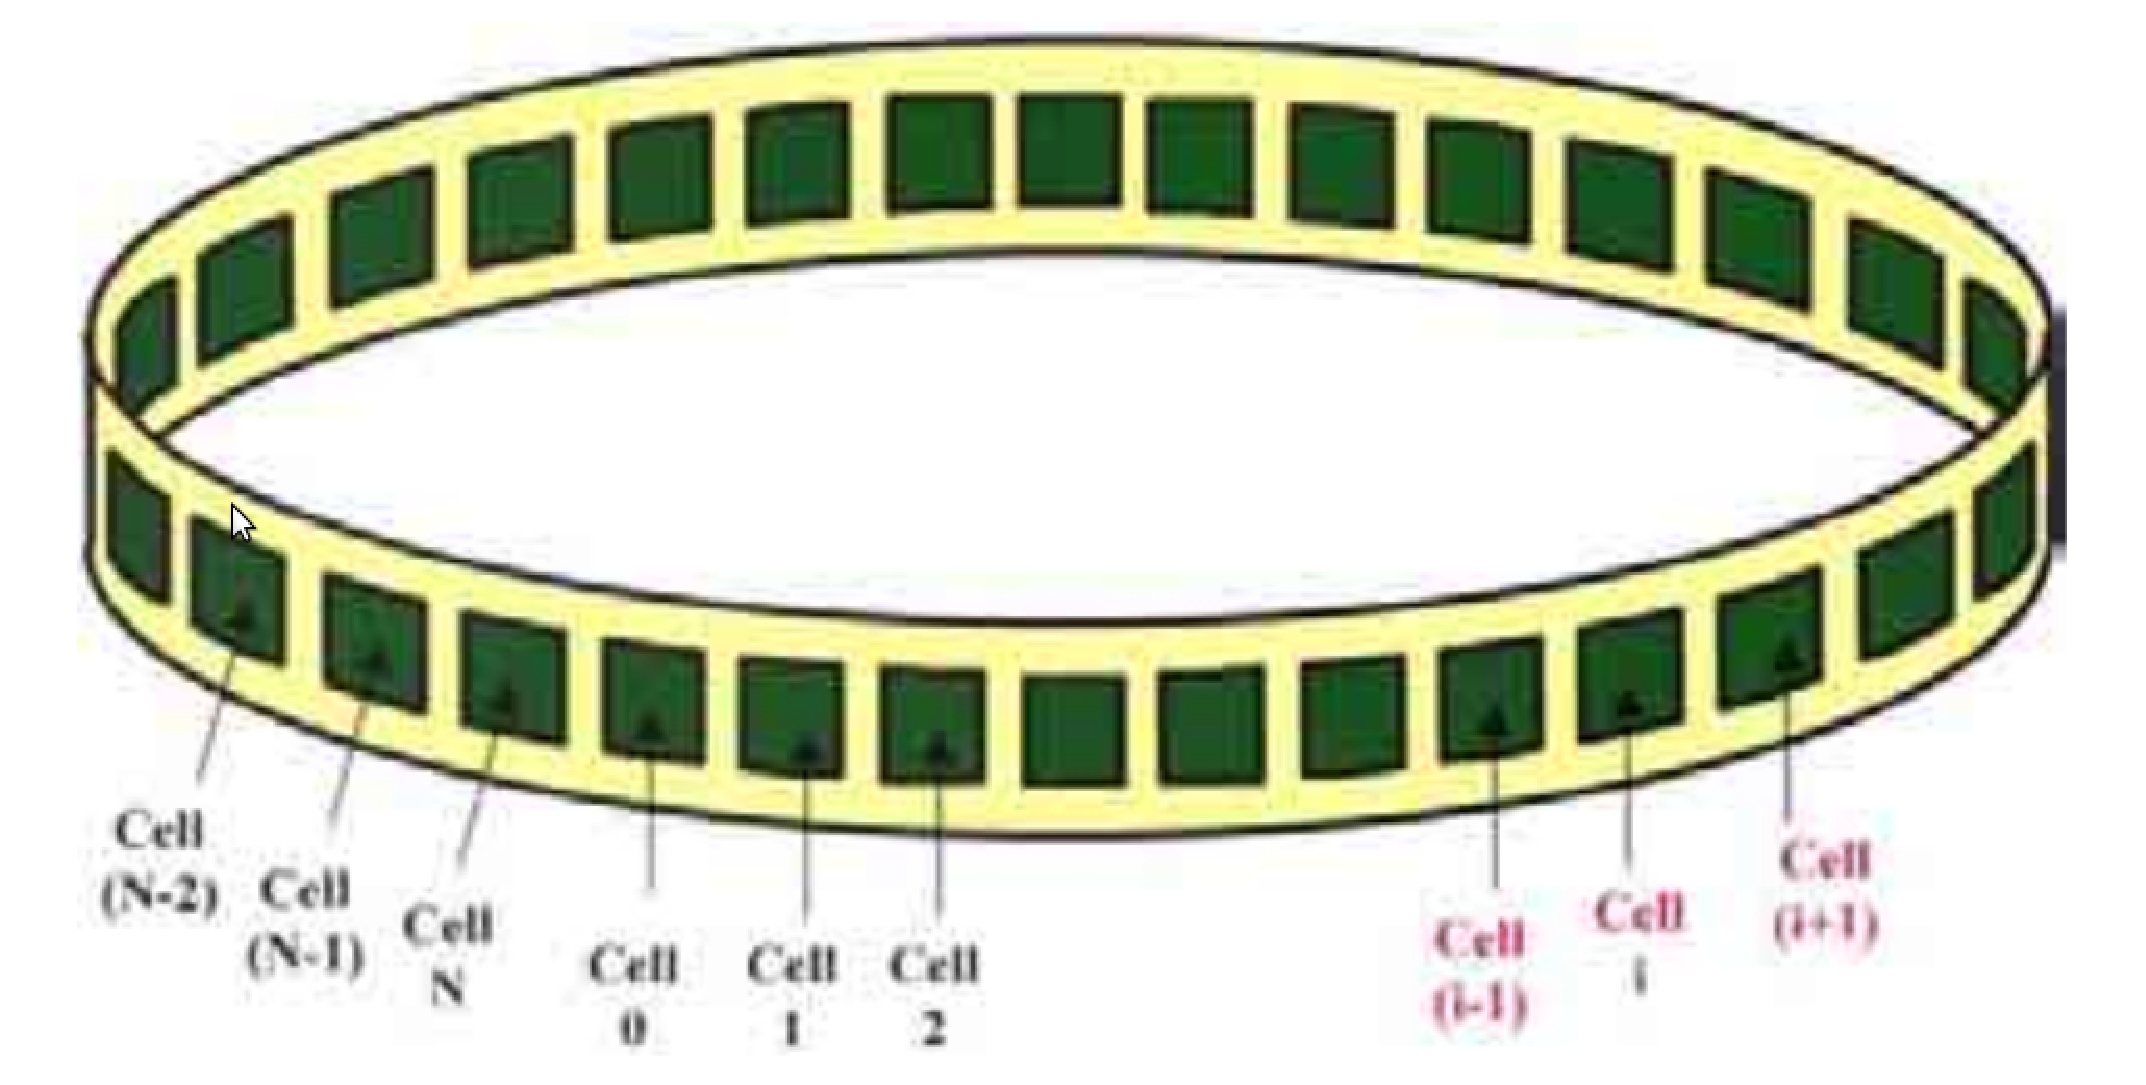
\includegraphics[scale=0.3]{img/ring.eps}
\caption{Condição de contorno periódica: a última célula é ligada à primeira,
formando um anel \citecustom{chua2002a}}
\label{fig:ring}
\end{center}
\end{figure}

A evolução de um autômato unidimensional pode ser visualizada por meio de uma grade bidimensional
onde cada linha representa uma configuração global em um determinado instante de tempo discreto,
conforme visualizado na Figura \ref{fig:celautomaton}.

\begin{figure}[htp]
\begin{center}
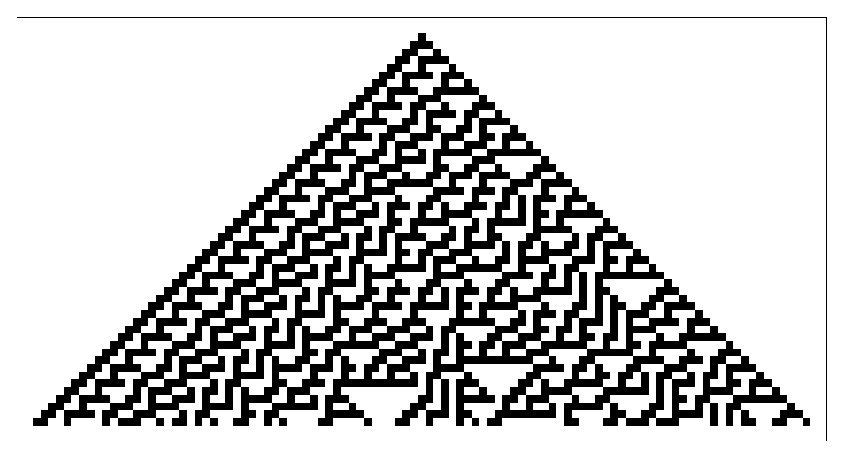
\includegraphics[scale=0.8]{img/CellularAutomaton.eps}
\caption{Evolução temporal de um autômato celular unidimensional}
\label{fig:celautomaton}
\end{center}
\end{figure}

Existem $2^3=8$ possíveis padrões de estados dentro de uma vizinhança para autômatos elementares.
Cada combinação pode resultar nos valores 0 ou 1, assim podem existir $2^{2^3}=256$ autômatos
celulares elementares. A regra local pode ser formalizada como:

\begin{equation}
x^{t+1}_i = \phi(x^t_{i-1}, x^t_i, x^t_{i+1})
\end{equation}

Onde $x^t_i$ é o estado da célula $i$ no instante $t$ em que a regra local atua, e $\phi$ é a função
que executa a regra local.  A Tabela \ref{tab:localrule} mostra como é aplicada a regra local.
As regras locais para autômatos elementares podem ser descritas por um número número binário de
oito dígitos, codificado pelo resultado das oito combinações de vizinhança da regra local
\citecustom{wolfram1983}. No caso da Figura \ref{fig:celnumbering}, este número é o número $90_{10}$, e
este autômato é chamado de \textit{regra 90}.

\begin{table}[htp]
\begin{center}
\begin{tabular}{|c|c|c|c|}
\hline
\Large $x_{i-1}$ & \Large $x_i$ & \Large $x_{i+1}$ & \Large $\phi$ \\ \hline
1 & 1 & 1 & 0 \\ \hline
1 & 1 & 0 & 1 \\ \hline
1 & 0 & 1 & 0 \\ \hline
1 & 0 & 0 & 1 \\ \hline
0 & 1 & 1 & 1 \\ \hline
0 & 1 & 0 & 0 \\ \hline
0 & 0 & 1 & 1 \\ \hline
0 & 0 & 0 & 0 \\ \hline
\end{tabular}
\caption{Aplicação de regra local}
\label{tab:localrule}
\end{center}
\end{table}

\begin{figure}[htp]
\begin{center}
\[ \fbox {
{\Large
\begin{tabular}{c c c c c c c c c c c}
$\frac{1 1 1}{0}$ & $\frac{1 1 0}{1}$ & $\frac{1 0 1}{0}$ & $\frac{1 0 0}{1}$ & 
$\frac{0 1 1}{1}$ & $\frac{0 1 0}{0}$ & $\frac{0 0 1}{1}$ & $\frac{0 0 0}{0}$ &
= & 90
\end{tabular}
}
} \]
\caption{Exemplo de esquema de numeração de Wolfram para autômatos celulares unidimensionais
\citecustom{wolfram1983}.}
\label{fig:celnumbering}
\end{center}
\end{figure}

\subsection{Equivalência de regras}

Duas regras locais ${\phi}_1$ e ${\phi}_2$ são ditas equivalentes se e somente se existir
uma transformação a qual mapeia a regra ${\phi}_1$ na regra ${\phi}_2$, e vice-versa
\citecustom{chua2002a}. Estas transformações podem ser de três tipos:

\begin{description}

\item[Transformação de complemento] nesta transformação todos os estados são complementados,
ou seja, troca-se 0 por 1 e vice-versa, conforme exemplificado na Figura \ref{fig:complement}.

\begin{figure}[htp]
\begin{center}
\begin{tabular}{|c|c|c|c|c|c|c|c|c|}
\hline
\Large \textbf{Vizinhança}  & 111 & 110 & 101 & 100 & 011 & 010 & 001 & 000 \\ \hline
\Large \textbf{$\phi$}      &  0  &  1  &  1  &  0  &  1  &  1  &  1  &  0  \\ \hline
\hline
\Large \textbf{Complemento} & 000 & 001 & 010 & 011 & 100 & 101 & 110 & 111 \\ \hline
\Large \textbf{$\phi$}      &  1  &  0  &  0  &  1  &  0  &  0  &  0  &  1  \\ \hline
\hline
\Large \textbf{Reordenado}  & 111 & 110 & 101 & 100 & 011 & 010 & 001 & 000 \\ \hline
\Large \textbf{$\phi$}      &  1  &  0  &  0  &  0  &  1  &  0  &  0  &  1  \\ \hline
\end{tabular}
\caption{Transformação de complemento}
\label{fig:complement}
\end{center}
\end{figure}

\item[Transformação por reflexão] nesta transformação o estado do vizinho da direita é
trocado com o estado do vizinho da esquerda. A Figura \ref{fig:reflex} ilustra o processo.

\begin{figure}[htp]
\begin{center}
\begin{tabular}{|c|c|c|c|c|c|c|c|c|}
\hline
\Large \textbf{Vizinhança}  & 111 & 110 & 101 & 100 & 011 & 010 & 001 & 000 \\ \hline
\Large \textbf{$\phi$}      &  0  &  1  &  1  &  0  &  1  &  1  &  1  &  0  \\ \hline
\hline
\Large \textbf{Reflexão}    & 111 & 001 & 101 & 011 & 100 & 010 & 110 & 000 \\ \hline
\Large \textbf{$\phi$}      &  0  &  1  &  1  &  0  &  1  &  1  &  1  &  0  \\ \hline
\hline
\Large \textbf{Reordenado}  & 111 & 110 & 101 & 100 & 011 & 010 & 001 & 000 \\ \hline
\Large \textbf{$\phi$}      &  0  &  1  &  1  &  1  &  0  &  1  &  1  &  0  \\ \hline
\end{tabular}
\caption{Transformação do tipo reflexão}
\label{fig:reflex}
\end{center}
\end{figure}

\item[Transformação conjunta] neste caso é realizada uma operação conjunta das duas
operações anteriores.

\end{description}

Para os 256 autômatos celulares elementares, existem 88 classes de regras equivalentes.
A Tabela \ref{tab:equiv} lista todas as classes de equivalência. A classe com o menor número
de regra é escolhida como representante de classe.

\begin{table}[H]
\begin{minipage}[b]{0.3\linewidth}\centering
\begin{tabular}{|c|c|}
\hline
\footnotesize Representante & \footnotesize Regras \\
{\footnotesize da classe} & \footnotesize equivalentes \\ \hline
0   & 255 \\ \hline
1   & 127 \\ \hline
2   & 16,191,247 \\ \hline
3   & 17,63,119 \\ \hline
4   & 223 \\ \hline
5   & 95 \\ \hline
6   & 20,159,215 \\ \hline
7   & 21,431,87 \\ \hline
8   & 64,239,253 \\ \hline
9   & 65,111,125 \\ \hline
10  & 80,175,245 \\ \hline
11  & 47,81,117 \\ \hline
12  & 68,207,221 \\ \hline
13  & 69,79,93 \\ \hline
14  & 84,143,213 \\ \hline
15  & 85 \\ \hline
18  & 183 \\ \hline
19  & 55 \\ \hline
22  & 151 \\ \hline
23  & \\ \hline
24  & 66,189,231 \\ \hline
25  & 61,67,103 \\ \hline
26  & 82,167,181 \\ \hline
27  & 39,53,83 \\ \hline
28  & 70,157,199 \\ \hline
29  & 71 \\ \hline
30  & 86,135,149 \\ \hline
32  & 251 \\ \hline
33  & 123 \\ \hline
34  & 48,187,243 \\ \hline
\end{tabular}
\end{minipage}
\hspace{0.3cm}
\begin{minipage}[b]{0.3\linewidth}
\centering
\begin{tabular}{|c|c|}
\hline
\footnotesize Representante & \footnotesize Regras \\
{\footnotesize da classe} & \footnotesize equivalentes \\ \hline
35  & 49,59,115 \\ \hline
36  & 219 \\ \hline
37  & 91 \\ \hline
38  & 52,155,211 \\ \hline
40  & 96,235,249 \\ \hline
41  & 97,107,121 \\ \hline
42  & 112,171,241 \\ \hline
43  & 113 \\ \hline
44  & 100,203,217 \\ \hline
45  & 75,89,101 \\ \hline
46  & 116,139,209 \\ \hline
50  & 179 \\ \hline
51  & \\ \hline
54  & 147 \\ \hline
56  & 98,185,227 \\ \hline
57  & 99 \\ \hline
58  & 114,163,177 \\ \hline
60  & 102,153,195 \\ \hline
62  & 118,131,145 \\ \hline
72  & 237 \\ \hline
73  & 109 \\ \hline
74  & 88,173,229 \\ \hline
76  & 205 \\ \hline
77  & \\ \hline
78  & 92,141,197 \\ \hline
90  & 165 \\ \hline
94  & 133 \\ \hline
104 & 233 \\ \hline
105 & \\ \hline
106 & 120,169,225 \\ \hline
\end{tabular}
\end{minipage}
\hspace{0.3cm}
\begin{minipage}[b]{0.3\linewidth}
\centering
\begin{tabular}{|c|c|}
\hline
\footnotesize Representante & \footnotesize Regras \\
{\footnotesize da classe} & \footnotesize equivalentes \\ \hline
108 & 201 \\ \hline
110 & 124,137,193 \\ \hline
122 & 161 \\ \hline
126 & 129 \\ \hline
128 & 254 \\ \hline
130 & 144,190,246 \\ \hline
132 & 222 \\ \hline
134 & 148,158,214 \\ \hline
136 & 192,238,252 \\ \hline
138 & 174,208,244 \\ \hline
140 & 196,206,220 \\ \hline
142 & 212 \\ \hline
146 & 182 \\ \hline
150 & \\ \hline
152 & 188,194,230 \\ \hline
154 & 166,180,210 \\ \hline
156 & 198 \\ \hline
160 & 250 \\ \hline
162 & 176,186,242 \\ \hline
164 & 218 \\ \hline
168 & 224,234,248 \\ \hline
170 & 240 \\ \hline
172 & 202,216,228 \\ \hline
178 & \\ \hline
184 & 226 \\ \hline
200 & 236 \\ \hline
204 & \\ \hline
232 & \\ \hline
& \\ \hline
& \\ \hline
\end{tabular}
\end{minipage}
\caption{Autômatos celulares elementares equivalentes \citecustom{wolfram1994}}
\label{tab:equiv}
\end{table}

As Figuras \ref{fig:rule30} e \ref{fig:rule86} mostram a evolução de duas regras locais
equivalentes. Nota-se pelas figuras que a evolução de uma é o espelho da outra.

\begin{figure}[ht]
\begin{minipage}[b]{0.5\linewidth}
\centering
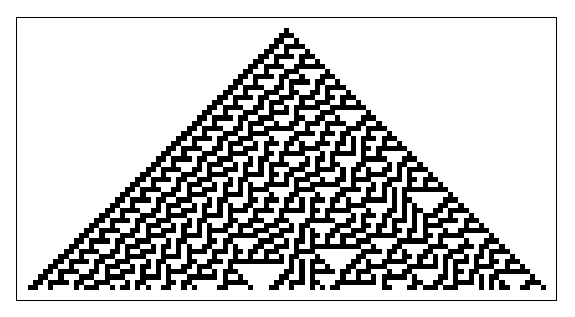
\includegraphics[scale=0.85]{img/rule30.eps}
\caption{Regra 30}
\label{fig:rule30}
\end{minipage}
\hspace{0.5cm}
\begin{minipage}[b]{0.5\linewidth}
\centering
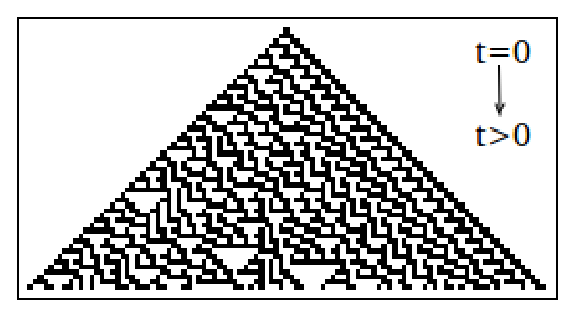
\includegraphics[scale=0.85]{img/rule86.eps}
\caption{Regra 86}
\label{fig:rule86}
\end{minipage}
\end{figure}

Estudar as classes de equivalência mostra-se importante porque regras locais
equivalentes apresentam o mesmo padrão de complexidade de evolução.

\subsection{Classificação dos autômatos celulares}

\citeonline{wolfram1994} dividiu os autômatos celulares elementares em quatro
classes segundo a complexidade do padrão gerado pelo seu comportamento dinâmico,
conforme descrito a seguir:

\begin{description}
\item[Classe 1] a evolução leva a um estado homogêneo (ponto fixo).
\item[Classe 2] a evolução leva a um conjunto de estruturas periódicas.
\item[Classe 3] a evolução leva a um padrão caótico.
\item[Classe 4] a evolução leva a estruturas localizadas complexas.
\end{description}

Os atratores nas classes 1, 2 e 3 são respectivamente análogos aos atratores
de ponto fixo, ciclo limite e caóticos encontrados em sistemas dinâmicos
contínuos. A Figura \ref{fig:classes} mostra exemplos de autômatos celulares
das quatro classes de complexidade.

\begin{figure}[htp]
\begin{center}
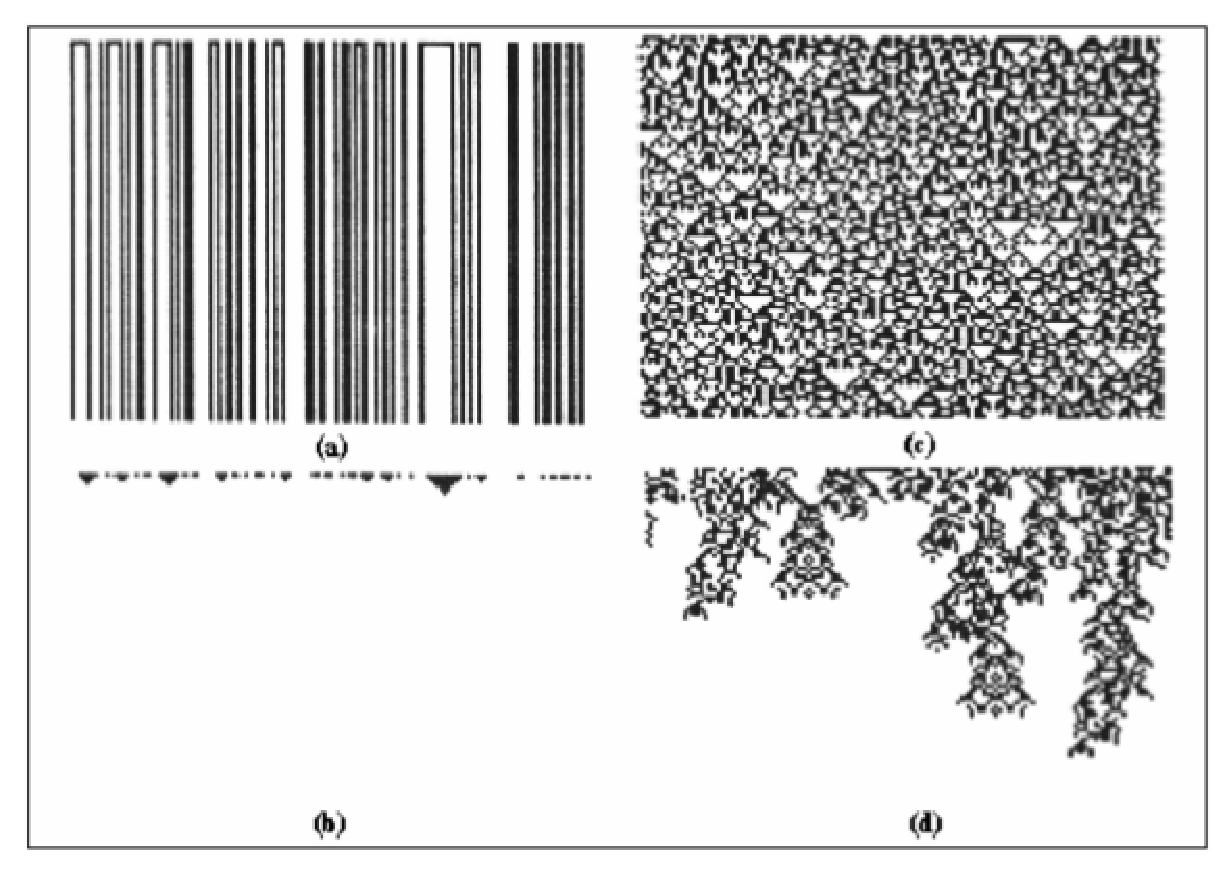
\includegraphics[scale=0.5]{img/classes.eps}
\caption{Classes dinâmicas dos autômatos celulares \citecustom{wolfram1984}.
(a) classe 1, (b) classe 2, (c) classe 3 e (d) classe 4}
\label{fig:classes}
\end{center}
\end{figure}

Trabalhos posteriores se concentraram em formalizar a classificação intuitiva
feita por Wolfram \citecustom{sarkar2000}. \citeonline{culik1988} propuseram a seguinte
classificação.  Seja $\rho$ a regra local para o autômato celular, então:

\begin{enumerate}
\item A regra $\rho$ está na classe um se e somente se toda configuração finita,
isto é, configurações nas quais somente um número finito de células são em
estados não quiescentes, evoluem para uma configuração estável em muitos passos
finitos.

\item A regra $\rho$ está na classe dois se e somente se toda configuração finita
evolui para uma configuração periódica em um número finito de passos.

\item A regra $\rho$ está na classe três se e somente se é decidível se a
configuração ocorre na órbita de outra.

\item A classe quatro engloba todas as regras locais.
\end{enumerate}

\subsection{Autômatos finitos e comportamento limite}

A teoria dos autômatos é o estudo dos dispositivos de computação abstratos,
ou \textit{máquinas}. Antes de existirem computadores, na década de 1930, Alan
Turing estudou uma máquina abstrata que tinha todas as características dos
computadores atuais, pelo menos no que se refere ao quanto eles poderiam 
calcular. O objetivo de Turing era descrever com exatidão o limite entre
o que uma máquina de computação podia fazer e aquilo que ela não podia fazer.

Nas décadas de 1940 e 1950, tipos de máquinas mais simples, que hoje são
conhecidas como \textit{autômatos finitos}, foram estudados por diversos
pesquisadores. Esses autômatos, propostos originalmente para modelar a
função do cérebro, se mostraram extremamente úteis para uma grande variedade
de propósitos. Também no final dos anos 50, o linguista N. Chomsky, iniciou
o estudo de gramáticas formais. Embora não sejam estritamente máquinas,
essas gramáticas têm relacionamentos estreitos com os autômatos abstratos
\citecustom{hopcroft2002}.

Linguagens regulares estão entre os tópicos mais antigos em teoria de
linguagens formais. O estudo formal de linguagens regulares
e autômatos finitos é datado do início da década de 40, quando máquinas
de estado finito foram utilizadas para modelar conjuntos de neurônios
por McCulloch e Pitts. Desde então, linguagens regulares têm sido
extensivamente estudadas. Resultados das primeiras investigações são,
por exemplo, o teorema de Kleene estabelecendo a equivalência de
expressões regulares e autômatos finitos, a introdução de autômatos
com saída por Mealy e Moore, a introdução de autômatos finitos não
determinísticos por Rabin e Scott, e a caracterização de linguagens
regulares por congruência de índices finitos por Myhill e Nerode
\citecustom{rozenberg1997}.

O elemento básico de uma linguagem é o alfabeto, um conjunto finito de símbolos
utilizados para formar as palavras pertencentes à linguagem. Por exemplo, o
alfabeto $\Sigma = \{0,1\}$ contém os símbolos $0$ e $1$, e todas as palavras
formadas a partir deste alfabeto só poderão conter estes símbolos.

Uma palavra ou cadeia sobre um alfabeto é uma sequência finita de símbolos
pertencentes a este alfabeto. Assim, $011101$ é uma palavra sobre o alfabeto
$\Sigma = \{0, 1\}$. Uma palavra pode não conter nenhum símbolo. Neste caso,
ela recebe o nome de cadeia \textit{vazia}, e é denotada por $\varepsilon$.
O conjunto de todas as palavras não vazias sobre um alfabeto $\Sigma$ é
denotado por $\Sigma^+$, e o conjunto de todas as palavras, incluindo
a cadeia vazia, sobre um alfabeto $\Sigma$ é denotado por
${\Sigma}^+ \bigcup \varepsilon = \Sigma^*$. O comprimento de uma palavra
é o número de símbolos que a forma. Logo, o comprimento da palavra
\emph{abcd} é 4. Denota-se o comprimento de uma cadeia $w$ por
$|w|$; portanto, $|101| = 3$ e $|\varepsilon| = 0$. Alternativamente,
através de um isomorfismo natural, uma cadeia $w \in \Sigma^*$ pode ser
considerada como uma função $w: \{1,\cdots,|w|\} \mapsto \Sigma$; o
valor de $w(j)$, onde $1 \le j \le |w|$ é o símbolo que ocupa a j-ésima
posição em $w$ \citecustom{lewis2008}.

Dá-se o nome de \textbf{linguagem} a qualquer conjunto de palavras sobre um
alfabeto $\Sigma$, ou seja, a qualquer subconjunto de $\Sigma^*$. Portanto,
$\Sigma^*$, $\emptyset$ e $\Sigma$ são linguagens. Sendo uma linguagem 
simplesmente um tipo particular de conjunto, pode-se especificar linguagens
finitas enumerando-se todas as suas palavras. Por exemplo, $\{aba, czr, d, f\}$
é uma linguagem sobre $\{a, b, \cdots, z\}$. Entretanto, a maioria das
linguagens são infinitas, não sendo portanto possível listar todas as palavras
\citecustom{lewis2008}. Assim, especifica-se linguagens infinitas da seguinte forma:

\begin{center}
$L = \{w \in \Sigma^*: \mbox{ w possui a propriedade P}\}$
\end{center}

Nota-se que uma linguagem sobre $\Sigma$ não precisa incluir palavras com todos
os símbolos de $\Sigma$; assim, uma vez que se estabelece que $L$ é uma
linguagem sobre $\Sigma$, também sabe-se que ela é uma linguagem sobre qualquer
alfabeto que seja um superconjunto de $\Sigma$ \citecustom{hopcroft2002}.

\subsection{Autômatos finitos e linguagens regulares}

Segundo \citeonline{hopcroft2002}, um autômato finito é definido por
uma quíntupla $A = (\mathbb{Q},\Sigma,\delta,q_0,\mathbb{F})$, onde:

\begin{description}
\item[$A$] é o nome associado ao autômato finito.
\item[$\mathbb{Q}$] é um conjunto finito de estados.
\item[$\Sigma$] é um conjunto finito de símbolos de entrada
\item[$\delta$] é uma função de transição do tipo $\delta: \mathbb{Q} \times \Sigma \mapsto \mathbb{Q}$.
A função de transição toma um estado e um símbolo de entrada e retorna um novo estado.
$\delta$ também é chamada de \textit{tabela de transição de estados}.
\item[$q_0$] é o estado inicial.
\item[$\mathbb{F}$] é o conjunto de estado finais. $\mathbb{F} \subseteq \mathbb{Q}$.
\end{description}

O autômato atua lendo símbolos de uma fita de entrada onde cada posição na fita
contém um símbolo. O autômato começa seu processamento no estado inicial $q_0$ e,
a cada símbolo lido da fita de entrada, a função de transição
$\delta: \mathbb{Q} \times \Sigma \mapsto \mathbb{Q}$ define um novo estado como o estado atual.
Quando o processamento da fita de entrada termina, se o estado atual for
um dos estados pertencentes ao conjunto $F$ de estados finais, a entrada é
considerada aceita, caso o contrário, a entrada é rejeitada. Por exemplo,
considere o seguinte autômato finito:

\begin{center}
$M = \{ \mathbb{Q} = \{A,B\}, \break \Sigma = \{0,1\}, \break
\delta = \{A \times 0 \mapsto A; A \times 1 \mapsto B; B \times 0 \mapsto A; B \times 1 \mapsto B\}, \break
q_0 = A, \break \mathbb{F} = \{B\} \}$
\end{center}

Neste caso, o estado inicial é o estado $A$, e o conjunto de estados finais
é formado pelo estado único $B$. É fácil verificar que este autômato aceita
qualquer palavra sobre o alfabeto $\{0,1\}$ que termine com o símbolo $1$.
Considere a cadeia $00101$. O autômato começa no estado $A$ e lê o primeiro
símbolo $0$, a função $\delta$ possui uma entrada $A \times 0 \mapsto A$,
então o autômato consome o símbolo $0$, avança a fita de entrada e permanece
no estado $A$. Novamente um $0$ é lido, então o estado $A$ é mantido e
avança-se a fita de entrada. Agora o símbolo $1$ é lido, a entrada correspondente
na tabela de transição é $A \times 1 \mapsto B$, então o autômato vai para
o estado $B$. O próximo símbolo da entrada é o $0$, e a entrada correspondente
na tabela de transição é $B \times 0 \mapsto A$, então o autômato vai para o
estado $A$. O último símbolo de entrada é o símbolo $1$, então o autômato vai
para o estado $B$. Como toda a entrada foi consumida e o estado atual $B$
pertence ao conjunto de estados finais $F$, a cadeia de entrada $00101$ é
aceita.

Autômatos finitos também podem ser representados graficamente através de
um grafo orientado. Os estados são representados pelos nós do grafo
e os arcos representam as transições de estado. O estado inicial possui
uma seta de entrada e os estados finais possui um círculo duplo. A
Figura \ref{fig:automata} mostra graficamente o autômato anterior.

\begin{figure}[htp]
\begin{center}
\begin{VCPicture}{(0,-2)(3,2)}
\State[A]{(0,0)}{A} \FinalState[B]{(3,0)}{B}
\Initial{A} %\Final{B}
\ArcL{A}{B}{1} \ArcL{B}{A}{0}
\LoopN{A}{0} \LoopN{B}{1}
\end{VCPicture}
\caption{Autômato finito representado como um grafo orientado.}
\label{fig:automata}
\end{center}
\end{figure}

O autômato finito anteriormente exemplificado é chamado de autômato finito determinístico.
Em um autômato finito determinístico, cada transição na função de transição possui apenas
um único estado objetivo, ou seja, cada entrada da tabela de transição possui a forma
$\delta: (q, s) \in (\mathbb{Q},\Sigma) \mapsto q' \in \mathbb{Q}$. Nos autômatos finitos não
determinísticos, cada entrada na tabela de transição é da forma
$\delta: (q, s) \in (\mathbb{Q},\Sigma) \mapsto \mathbb{Q}' \subseteq \mathbb{Q}$,
ou seja, para um dado estado e um símbolo de entrada, o número de possíveis
transições pode ser maior que um. \citecustom{rozenberg1997}.  Um autômato não
determinístico também pode possuir mais de um estado inicial.

O processamento em um autômato não determinístico é análogo à sua contraparte
determinística, exceto que quando existe um ambiguidade na transição (existe
mais de um estado objetivo para um dada entrada) o autômato se replica, tomando
o caminho dos $n$ estados objetivos. A entrada é considerada aceita se, ao
final do processamento, pelo menos uma instância do autômato está em um
estado final.

O conjunto de palavras reconhecidas por um autômato forma a linguagem do
autômato. Seja $M$ um autômato, $L(M)$ constitui sua linguagem. A classe
de linguagens reconhecidas por autômatos finitos são as linguagens regulares.
Linguagens regulares podem também ser representadas por meio das chamadas
expressões regulares. Uma expressão regular é construída a partir dos
seguintes elementos \citecustom{trafaniuc2004}:

\begin{enumerate}
\item O alfabeto de símbolos $\sigma \in \Sigma$;
\item $xy$ representa a concatenação de $x$ e $y$;
\item $x+y$ representa $x$ ou $y$;
\item $x^+$ representa uma ou mais concatenações de $x$;
\item $x^*$ representa qualquer número de concatenações de $x$, incluindo
nenhuma (o que representa a cadeia vazia).
\end{enumerate}

Por exemplo, a expressão regular do autômato da Figura \ref{fig:automata}
é $(0+1)^*1^+$.

\subsection{Evolução de um autômato celular}

Linguagens formais consistem do conjunto de palavras formadas a partir de
cadeias de símbolos em um alfabeto finito $\mathbb{S}$ de acordo com regras
gramaticas definidas. Conjuntos de configurações de autômatos celulares
podem assim ser considerados como linguagens formais, com cada palavra na
linguagem representando uma configuração do autômato celular. Tais conjuntos
infinitos de configurações são então completamente especificados por
conjuntos finitos de regras gramaticais \citecustom{wolfram1984}.

Os atratores das classes 1 e 2 de autômatos celulares elementares podem ser
representados por linguagens regulares simples. Os atratores da classe 3 podem
ser representados por linguagens regulares mais complexas. Os atratores da
classe 4 podem ou não ser representados por uma linguagem regular \citecustom{li1987}.

O conjunto de configurações possíveis em um autômatos celular depois de $t$
passos de evolução pode ser representado por um conjunto $\Omega^{(t)}$.

O seguinte exemplo, retirado de \citecustom{wolfram1984}, ilustra o processo de
geração do autômato finito que representa o conjunto de configurações
possíveis $\Omega^{(t)}$ após $t$ iterações.

Considere a construção do conjunto $\Omega^{(1)}$ gerado por um passo de
tempo na evolução do autômato celular elementar com uma regra
local $\phi$ dada por (regra número 76):

\begin{equation}\label{eqn:r76}
111 \mapsto 0, 110 \mapsto 1, 101 \mapsto 0, 100 \mapsto 0, 011 \mapsto 1, 010 \mapsto 1,
001 \mapsto 0, 000 \mapsto 0
\end{equation}

O valor $a_i^{(1)}$ de uma célula na posição $i$ em uma configuração
$A^{(1)} = \phi A^{(0)} \in \Omega^{(1)}$ depende da vizinhança de três
células $\{a_{i-1}^{(0)},a_i^{(0)},a_{i+1}^{(0)}\}$ na configuração precedente
$A^{(0)} \in \Omega^{(0)}$. A célula adjacente de $a_{i+1}^{(1)}$ depende da
vizinhança sobreposta $\{a_i^{(0)},a_{i+1}^{(0)},a_{i+2}^{(0)}\}$. A
dependência de $a_{i+1}^{(0)}$ em $a_i^{(0)}$ associada com esta sobreposição
de duas células nas vizinhanças pode ser representada por um grafo $g$, conforme
ilustra a Figura \ref{fig:A1}. Os nós no grafo representam as sobreposições
$\{a_i^{(0)},a_{i+1}^{(0)}\}$. Este nós são agregados por arcos direcionados
correspondentes a vizinhanças de três células. A regra local do autômato
celular $\phi$ da Equação \ref{eqn:r76} define uma transformação para cada
vizinhança de três células, e assim associa um símbolo com cada arco de $g$.
Cada possível caminho através de $g$ corresponde a uma configuração particular
$A^{(0)}$. O sucessor $A^{(1)}$ de cada configuração inicial é dado pela
sequência de símbolos associada com os arcos no caminho. As sequências de
símbolos obtidas seguindo todos os caminhos possíveis através de $g$ assim
correspondem a todas as possíveis configurações $A^{(1)}$ obtidas depois
de um passo de tempo na evolução do autômato celular \ref{eqn:r76}. O
conjunto completo $\Omega^{(1)}$ pode assim ser representado pelo grafo
$g$. Está claro que nem todas as possíveis sequências de 0s e 1s podem
aparecer nas configurações de $\Omega^{(1)}$. Por exemplo, não existe um
caminho em $g$ que pode incluir a sequência $111$, e assim nenhuma
configuração em $\Omega^{(1)}$ pode conter blocos de células $111$.

\begin{figure}[htp]
\begin{center}
\begin{VCPicture}{(0,-2)(12,8)}
\State[00]{(0,3)}{A} \State[01]{(6,6)}{B}
\State[10]{(6,0)}{C} \State[11]{(12,3)}{D}
\ArcL{A}{B}{001 \mapsto 0} \LoopW{A}{000 \mapsto 0}
\ArcL{B}{D}{001 \mapsto 1} \ArcL{B}{C}{010 \mapsto 1}
\ArcL{C}{B}{101 \mapsto 0} \ArcL{C}{A}{100 \mapsto 0}
\ArcL{D}{C}{110 \mapsto 1} \LoopE{D}{111 \mapsto 0}
\end{VCPicture}
\caption{O grafo de transição de estados $g$ para um autômato finito
não determinístico que gera as configurações obtidas depois de um passo
de tempo na evolução do autômato celular com a regra número 76.
Possíveis sequências de valores de células são representadas por
caminhos possíveis pelo grafo. Os nós no grafo são rotulados por pares
de valores iniciais das células; os arcos então correspondem a triplas
de valores iniciais das células. Cada tripla é mapeada sob a regra 76
para um valor particular da célula. O grafo com arcos rotulados por estas
células correspondem a todas as configurações possíveis obtidas depois
de um passo de tempo \citecustom{wolfram1984}.}
\label{fig:A1}
\end{center}
\end{figure}

O grafo $g$ da Figura \ref{fig:A1} pode ser considerado como uma grafo
de transição de estados para um autômato finito o qual gera a linguagem
formal $\Omega^{(1)}$. Cada nó de $g$ corresponde a um estado do
autômato finito, e cada arco a uma transição no autômato finito, ou
equivalentemente a uma regra produção na gramática representada pelo
autômato finito. O conjunto $\Omega^{(1)}$ assim forma uma linguagem
regular.

\subsection{Semi-autômato}

O grafo da Figura \ref{fig:A1} é definido como um semi-autômato.
De acordo com \citeonline{miki2006}, um semi-autômato é um autômato
finito não determinístico, onde todos os estados da máquina são iniciais
e finais e é definido formalmente por uma tripla $\{\mathbb{Q},\Sigma,\delta\}$,
onde:

\begin{description}
\item[$\mathbb{Q}$] representa o conjunto de estados;
\item[$\Sigma$] é o alfabeto de símbolos;
\item[$\delta:\mathbb{Q} \times \Sigma \mapsto 2^\mathbb{Q}$] é a regra de transição, onde
$2^\mathbb{Q}$ é o conjunto potência de $\mathbb{Q}$ e pode ser representada na forma
$\delta(q,a) = \{p_1,p_2,p_3,\ldots,p_n\}$, onde $q$ é o estado atual, $a$
é o símbolo que a máquina lê, e $\{p_1,p_2,p_3,\ldots,p_n\}$ é o
conjunto de possíveis novos estados;
\end{description}

\subsection{Configuração inicial de um autômato celular}

O espaço de configurações iniciais $\Omega^{(0)}$ de um autômato celular
elementar pode ser qualquer combinação de sequências de 0s e 1s
representando os estados iniciais das células. O autômato finito
que representa tal sequência pode ser visualizado na Figura
\ref{fig:initconfigautomaton}, e sua representação em formato de
semi-autômato como implementado no \textit{software Mathematica}
na Figura \ref{fig:initconfigmathematica}.

\begin{figure}[htp]
\begin{center}
\begin{VCPicture}{(0,-2)(3,2)}
\FinalState[A]{(0,0)}{A}
\Initial{A}
\LoopN{A}{0,1}
\end{VCPicture}
\caption{Possíveis configurações iniciais representadas por um autômato finito
determinístico. É fácil perceber que o autômato aceita qualquer sequência de
0s e 1s.}
\label{fig:initconfigautomaton}
\end{center}
\end{figure}

\begin{figure}[htp]
\begin{center}
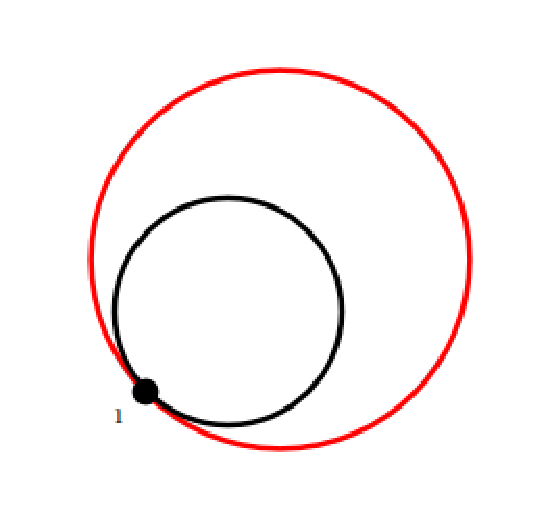
\includegraphics[scale=0.3]{img/InitialConfig.eps}
\caption{Semi-autômato representando as possíveis configurações iniciais
na notação do \textit{software Mathematica}. Arcos vermelhos representam
transições em 0 e arcos pretos representam transições em 1.}
\label{fig:initconfigmathematica}
\end{center}
\end{figure}

Na representação do \textit{Mathematica}, transições em 0 são
representadas por arcos vermelhos e transições em 1 são
representadas por arcos pretos.

\subsection{Funções NetCAStep, TrimNet e MinNet}

\emph{NetCAStep}, \emph{TrimNet} e \emph{MinNet} \citecustom{wolfram2002} são
funções desenvolvidas no \textit{Mathematica} para gerar autômatos finitos
que representam a evolução para um passo de tempo de um autômato celular
elementar.

Dado um semi-autômato relacionado à configuração do autômato celular para
um instante de tempo $t$, a função \emph{NetCAStep} \citecustom{wolfram2002}
retorna um autômato finito relacionado ao instante de tempo $t+1$
\citecustom{miki2006}.

A função \emph{NetCAStep} gera como saída uma lista de transições
de estados correspondente a um autômato finito não determinístico.
Sobre a lista de transições de estado resultante da função
\emph{NetCAStep} é aplicada a função \emph{TrimNet}, que, por sua vez,
preserva todos os estados acessíveis por qualquer nó da rede
\citecustom{miki2006}.

É possível encontrar um autômato mínimo que representa um conjunto
de sequências. Isto pode ser feito criando primeiro um autômato
determinístico no qual no máximo um arco de cada valor sai de cada
nó, assim combinando nós equivalentes. Este procedimento é
executado pela função \emph{MinNet} \citecustom{wolfram2002}.

\subsection{Análise da complexidade de linguagens regulares de autômatos
finitos elementares}

\citeonline{mikietal2011} analisaram o padrão de crescimento de complexidade
de linguagens regulares representando as configurações de autômatos celulares
elementares.

Sobre as 256 regras elementares foi o aplicado o algoritmo desenvolvido
por \citeonline{trafaniuc2004} ilustrado na Figura \ref{fig:rulesel} para
seleção de regras que apresentam autômatos finitos com crescimento de
complexidade a cada passo de tempo.

\begin{figure}[htp]
\begin{center}
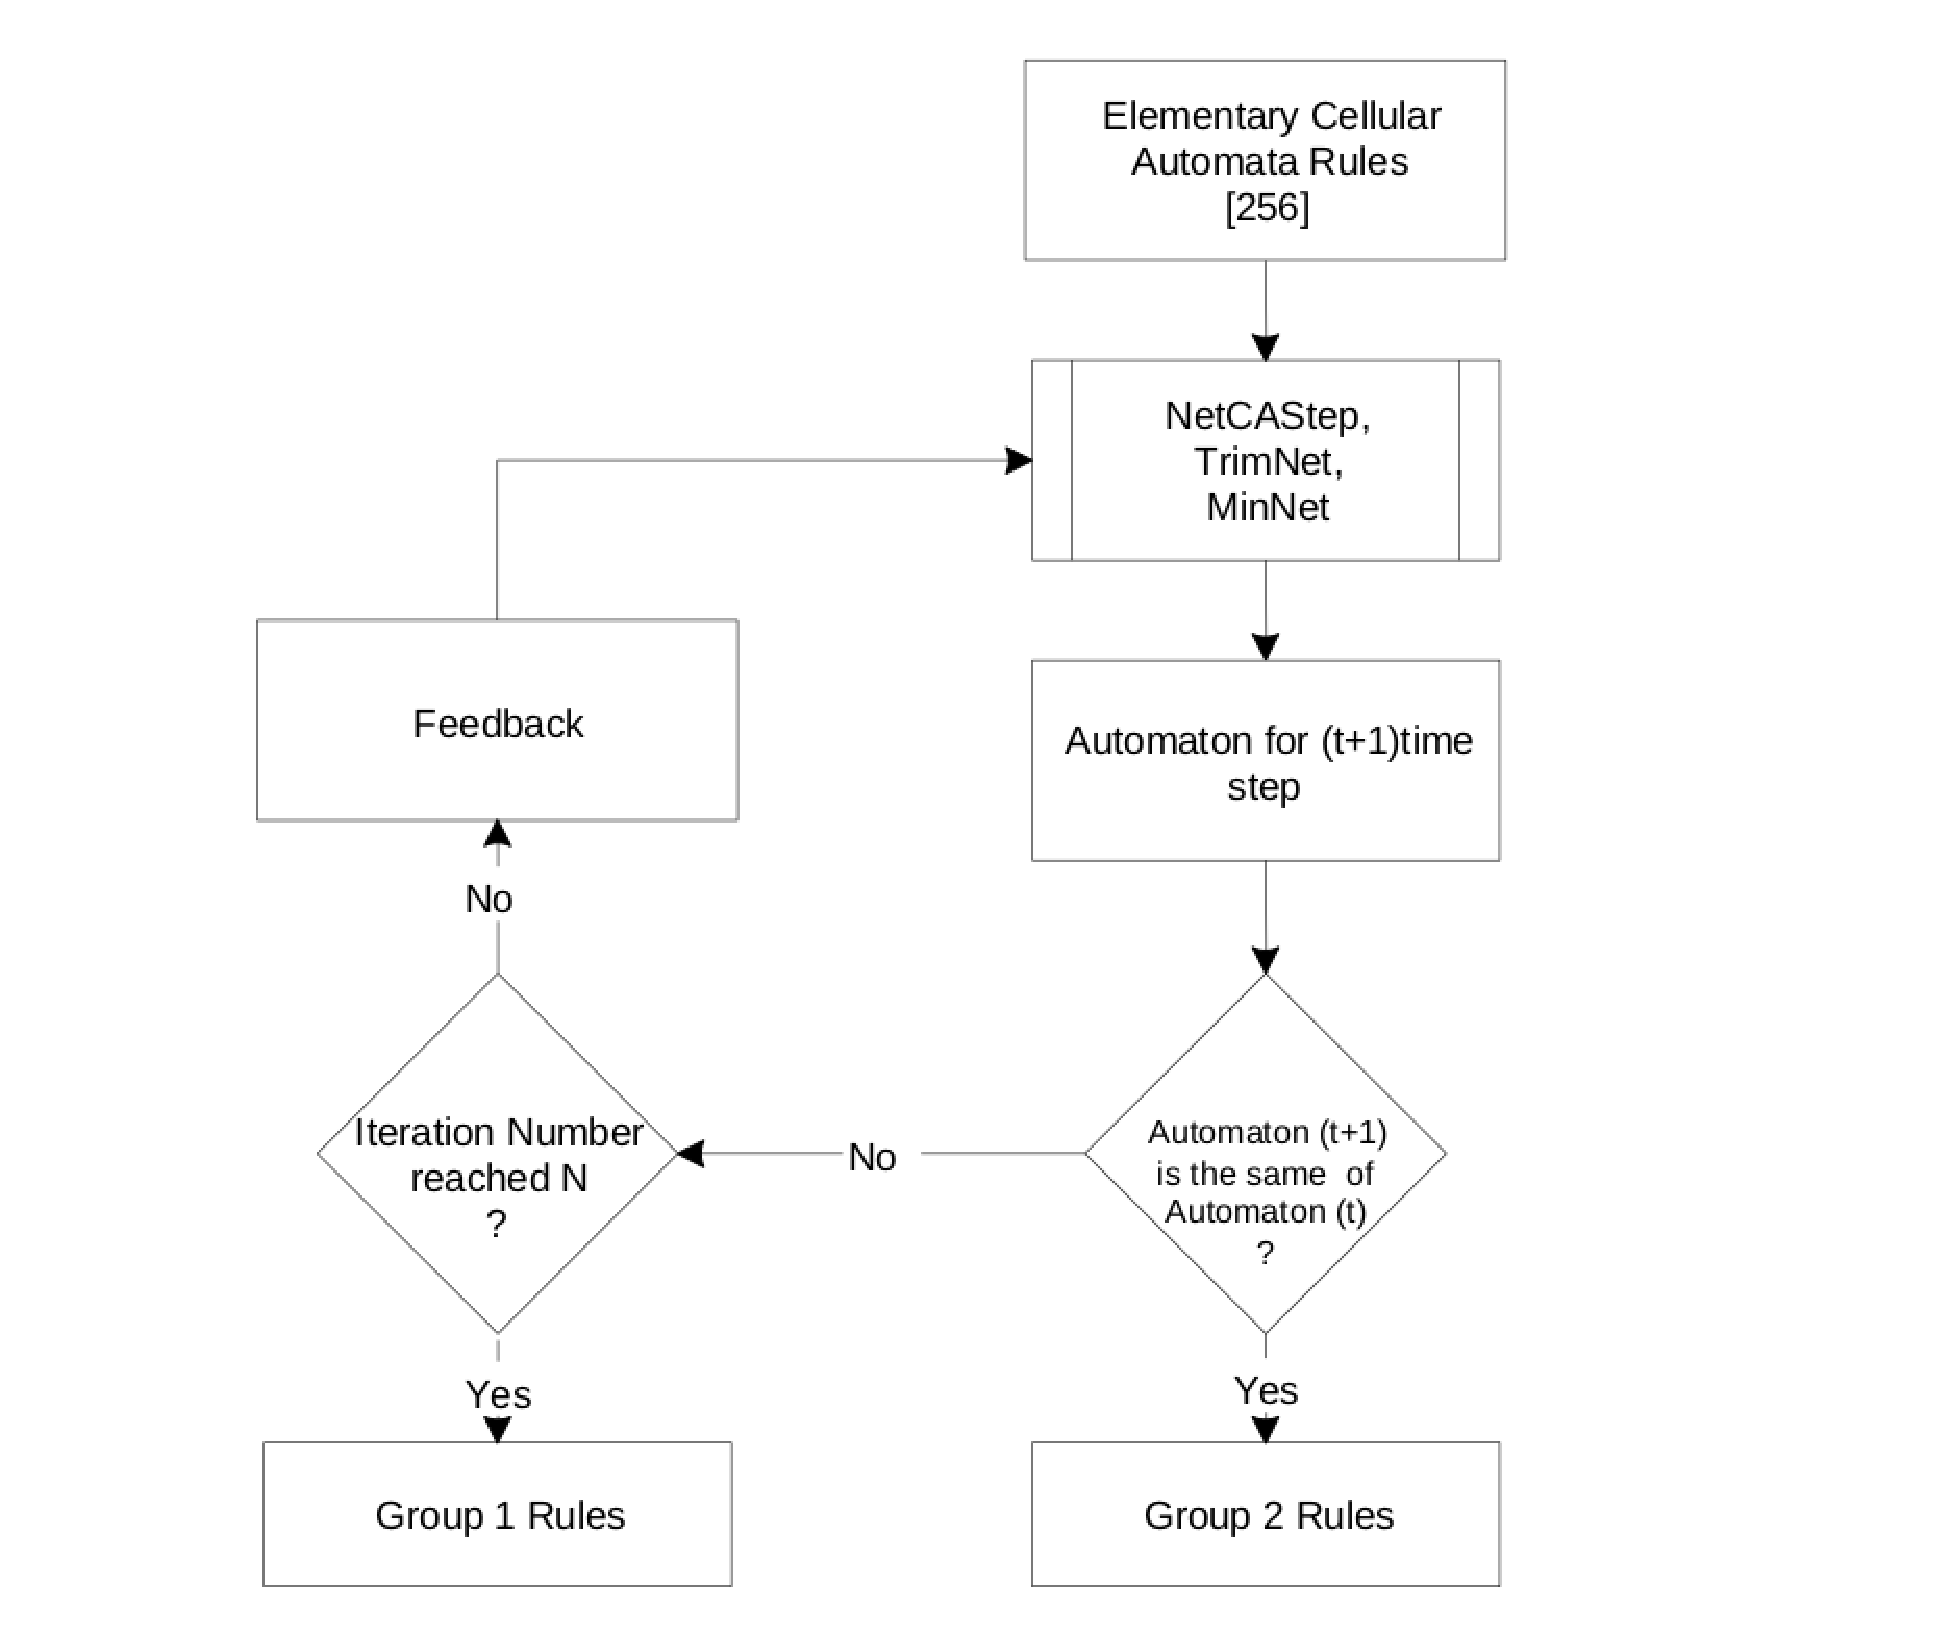
\includegraphics[scale=0.5]{img/rulesel.eps}
\caption{Algoritmo de seleção de regras \citecustom{mikietal2011}}
\label{fig:rulesel}
\end{center}
\end{figure}

O algoritmo divide as regras em dois grupos \citecustom{mikietal2011}:

\begin{description}
\item[Grupo 1] regras que apresentam crescimento de complexidade no autômato
finito limite a cada passo de tempo, e o método é interrompido quando o
número máximo de passos de execução for atingido.
\item[Grupo 2] regras que deixam de apresentar crescimento de complexidade no
autômato finito em até cinco passos de tempo.
\end{description}

O trabalho seguiu analisando os grafos gerados para diferentes instantes de tempo
das regras do grupo um onde percebeu-se que parte das estruturas dos autômatos
permaneciam inalteradas e repetitivas. Em busca de se obter expressões de crescimento
foi criado um método de identificação destas estruturas, com o objetivo de selecionar
regras com crescimento estruturado. O método é constituído em quatro passos
\citecustom{mikietal2011}:

\begin{enumerate}\label{sec:mikialgo}
\item Gerar os grafos das regras de transição, para dois passos de tempo
consecutivos, $t$ e $t+1$, de uma regra do espaço elementar.

\item Gerar todos os possíveis subgrafos do passo de tempo $t+1$ que tenham
o mesmo número de estados que o grafo do passo de tempo $t$.

\item Selecionar todos os subgrafos gerados com base no passo de tempo $t+1$
que se encaixam perfeitamente no grafo do passo de tempo $t$. Ou seja,
selecionar os subgrafos gerados no passo dois, que também são subgrafos do
grafo no tempo $t$.

\item Realizar uma operação de diferença entre o grafo de $t$ e todos os
subgrafos de $t+1$ selecionados no passo três, com o mesmo número de nós. O
subgrafo que apresentar a menor diferença no número de transições de estados
é selecionado. No caso de empate, o primeiro subgrafo é selecionado.
\end{enumerate}

Após a aplicação do método às regras do grupo um, foram identificados 26
conjuntos de regras agrupadas em classes de equivalência dinâmicas que
apresentaram estruturas comuns em passos de tempos consecutivos. Todas essas
26 classes foram então analisadas para obtenção de expressões
de crescimento, primeiro manualmente e depois com auxílio de um algoritmo
para sistematizar o processo \citecustom{mikietal2011}.

O trabalho reconstruiu a tabela de \citecustom{wolfram1994} e acrescentou novas
expressões de crescimento e outros resultados.

\section{Construção do semi-autômato por meio de matrizes de
adjacência}\label{sec:desenv}

Conforme já explicado anteriormente, o conjunto de configurações globais de
um autômato celular pode ser descrito por uma linguagem regular e,
consequentemente, por um autômato finito determinístico.

Estudos sobre a complexidade de autômatos celulares elementares por meio da
análise dos grafos dos autômatos finitos gerados pelas respectivas regras
foram realizados por \citeonline{miki2006} e por \citeonline{trafaniuc2004}.
Adicionalmente, estes estudos tentaram, sem sucesso, encontrar um algoritmo
que descrevesse a evolução dos autômatos das regras elementares (em
particular a regra 184) por meio da análise gráfica dos autômatos
finitos gerados pelo algoritmo de \citecustom{wolfram1984}.

Neste capítulo, é proposta uma nova abordagem para o problema, por meio da
análise das matrizes de adjacências correspondentes aos autômatos finitos
das respectivas regras do espaço elementar. Porém, como será visto adiante,
não é possível representar completamente um autômato finito utilizando a
notação clássica de matrizes de adjacências. É proposto, então, uma
nova notação que, dada a matriz de adjacência, é possível construir
integralmente o grafo da respectiva matriz.

O texto então deduz o algoritmo de formação do autômato finito
de tempo $t$ para a regra 184; e então finaliza com uma breve
descrição dos padrões de formação de matrizes das mesmas regras
estudados em \citecustom{mikietal2011}.

\subsection{Representação de semi-autômatos em forma matricial}

\subsubsection{Matrizes de adjacências}

Uma matriz de adjacências, algumas vezes também chamada de matriz de
conexões, representa os estados e transições de grafos em forma matricial,
rotulando as linhas e colunas com os vértices do grafo. As linhas e
colunas representam, respectivamente, os estados de origem e destino
do grafo\footnote{No caso de grafos não direcionados, não existe
distinção de estados origem e destino, mas somente grafos direcionados são 
de interesse neste trabalho}.

A representação de um grafo direcionado $G$ com $n$ vértices se dá por uma
matriz $M$ de tamanho $n \times n$. O valor da posição $a_{ij}$ da matriz
$M$ será $1$ se existir uma transição do estado $i$ para o estado $j$.
A Figura \ref{fig:graph} mostra um grafo direcionado e a Figura \ref{fig:adjm}
mostra a matriz de adjacências correspondente.

\begin{figure}[ht]
\begin{minipage}[b]{0.5\linewidth}
\begin{center}
\begin{VCPicture}{(0,-4)(4,1)}
\State[1]{(0,0)}{A} \State[2]{(4,0)}{B}
\State[3]{(2,-2)}{C}
\ArcL{A}{B}{} \ArcR{A}{C}{} 
\ArcL{B}{A}{}
\ArcR{C}{B}{} \LoopS{C}{}
\end{VCPicture}
\caption{Grafo direcionado}
\label{fig:graph}
\end{center}
\end{minipage}
\hspace{0.5cm}
\begin{minipage}[b]{0.5\linewidth}
\begin{center}
\begin{math}
\begin{pmatrix}
0 & 1 & 1 \\
1 & 0 & 0 \\
0 & 1 & 1
\end{pmatrix}
\end{math}
\caption{Representação em matriz de adjacências}
\label{fig:adjm}
\end{center}
\end{minipage}
\end{figure}

Embora matrizes de adjacências possam representar grafos direcionados simples,
não é possível representar completamente um semi-autômato, dado que:

\begin{enumerate}
\item É possível haver mais de uma transição do estado $i$ para o estado
$j$, $\exists i,j$.

\item Nos índices da matriz não está codificado o valor da transição, que
é o valor esperado na fita de entrada. Observe que a solução de criar
uma função $f: L \mapsto a_{ij}$ que associa o valor do arco ao índice
da matriz é inviável devido à possibilidade de existir mais de uma
transição por par de estados $(i,j)$.
\end{enumerate}

Para ilustrar a dificuldade de se representar semi-autômatos utilizando
matrizes de adjacências, considere o semi-autômato da Figura
\ref{fig:initconfigautomaton}. A matriz de adjacências deste autômato
seria uma matriz $1 \times 1$ com valor $a_{ij}=1$. Porém, perde-se a informação
de que existem duas transições reflexivas no semi-autômato. Mais ainda,
não existe qualquer menção ao valor das transições.

A próxima seção introduz uma notação alternativa de matrizes de
adjacências que contorna as duas dificuldades apresentados.

\subsubsection{Matrizes de adjacências isomórficas}

Uma matriz de adjacências isomórfica é uma notação de matriz de
adjacências para representar semi-autômatos que possui uma relação
de isomorfismo entre a matriz e sua representação em grafo.
Formalmente, dado o conjunto de matrizes de adjacências
isomórficas $\mathbb{M}$ e o conjunto de semi-autômatos $\mathbb{G}$,
existe uma transformação $T: \mathbb{G} \mapsto \mathbb{M}$ e uma
transformação $T^{-1}: \mathbb{M} \mapsto \mathbb{G}$. 

O elemento chave para conseguir essa relação de isomorfismo
é encontrar uma representação do conjunto de transições e
seus respectivos valores em um número real que possa ser codificado
nos índices da matriz, e que possa ser decodificado quando for
aplicada a transformação $T^{-1}$. Formalmente, dado o conjunto de transições
$\mathbb{L}$ do estado $i$ para o estado $j$, $\forall i,j$, encontrar uma
relação $\eta:\mathbb{L} \mapsto \Re$ que seja bijetora.

A resposta para esta questão está em criar um mapeamento dos valores
possíveis de transições para o conjunto de números naturais
$\mathbb{L} \mapsto \mathbb{N}$ e então codificar os valores das transições
em um número binário. Cada bit do número binário corresponde a um valor de
transição. Se o valor na $k$-ésima posição for 1, significa que existe uma
transição (mapeada no conjunto dos naturais) de valor $k$ do estado de
origem para o estado destino em questão. A operação $\eta$ de codificação dos
arcos $\mathbb{L}$ em um número real é o polinômio de base 2:

\begin{equation}
\eta(\mathbb{L}_{ij}) = \sum 2^k, \forall k \in (\mathbb{L}_{ij} \mapsto \mathbb{N})
\end{equation}

Onde $\mathbb{L}_{ij}$ é o conjunto de transições do estado $i$ para o estado
$j$. Repare que como $k \in \mathbb{N}$, então $\eta(\mathbb{L}_{ij}) \in \mathbb{Z}$,
ou seja, $\eta(\mathbb{L}_{ij})$ está restrita ao domínio dos inteiros. Se
$k \in \mathbb{Z}$ ($\mathbb{L}_{ij} \mapsto \mathbb{Z}$), então
$\eta(\mathbb{L}_{ij}) \in \Re$, pois admitiria-se a possibilidade de expoentes negativos.
Como computacionalmente é mais custoso trabalhar-se com números reais do que com inteiros,
e não há benefício aparente em expandir $\eta$ para o domínio dos reais,
já que $\mathbb{N}$ é contavelmente infinito \citecustom{lewis2008}, optou-se
por restringir-se ao domínio $\mathbb{Z}$ dos números inteiros.  A Figura \ref{fig:semigraph}
mostra o grafo da Figura \ref{fig:graph}, agora representado como um semi-autômato,
e a Figura \ref{fig:iadjm} mostra a matriz de adjacências isomórfica correspondente.

\begin{figure}[ht]
\begin{minipage}[b]{0.5\linewidth}
\begin{center}
\begin{VCPicture}{(0,-4)(4,1)}
\State[1]{(0,0)}{A} \State[2]{(4,0)}{B}
\State[3]{(2,-2)}{C}
\ArcL{A}{B}{0} \ArcR{A}{C}{0} 
\ArcL{B}{A}{1}
\ArcR{C}{B}{1} \LoopS{C}{0}
\end{VCPicture}
\caption{Semi-autômato representado através de um grafo direcionado}
\label{fig:semigraph}
\end{center}
\end{minipage}
\hspace{0.5cm}
\begin{minipage}[b]{0.5\linewidth}
\begin{center}
\begin{math}
\begin{pmatrix}
0 & 1 & 1 \\
2 & 0 & 0 \\
0 & 2 & 1
\end{pmatrix}
\end{math}
\caption{Representação em matriz de adjacências isomórfica}
\label{fig:iadjm}
\end{center}
\end{minipage}
\end{figure}

A transformação de um semi-autômato em uma matriz de adjacências
isomórfica é executada por meio do Algoritmo \ref{alg:stom}.

\begin{algorithm}
\caption{Algoritmo para gerar a matriz de adjacências isomórfica a partir
de um semi-autômato}
\label{alg:stom}
\begin{algorithmic}
\STATE $N \leftarrow \mbox{Length}(\mathbb{Q})$ \COMMENT{número de estados}
\STATE $A \leftarrow \mbox{ Matriz nula } N \times N$
\FORALL{$i,j \in \mathbb{Q}$}
\IF{$\mathbb{L}_{ij} \neq \emptyset$}
\STATE $A_{ij} = \eta(\mathbb{\mathbb{L}}_{ij})$
\ENDIF
\ENDFOR
\end{algorithmic}
\end{algorithm}

O algoritmo atua criando uma matriz $A_{N \times N}$, onde $N$ é o número
de estados do semi-autômato, e atribuindo à posição $A_{ij}$ o valor
da função $\eta(\mathbb{L}_{ij}),\forall i,j$, onde $\mathbb{L}_{ij}$
é o conjunto de transições de $i$ para $j$.

O algoritmo de transformação de uma matriz de adjacências isomórfica em
um semi-autômato é baseado na representação binária dos valores dos
índices da matriz. Por exemplo, se no índice $A_{1,2}$ existir o valor
$3$, então existe uma transição em $0$ e uma transição em $1$ do estado
\emph{1} para o estado \emph{2}, pois $2^0+2^1=3$. O Algoritmo \ref{alg:mtos}
mostra o processo de geração do semi-autômato a partir de uma matriz de
adjacências isomórfica. O algoritmo pressupõe a existência de uma função
\emph{MakeTransition(i,j,n)} que cria uma transição em \emph{n} do estado
\emph{i} para o estado \emph{j}.

\begin{algorithm}
\caption{Algoritmo para gerar o semi-autômato a partir de uma matriz de
adjacências isomórfica}
\label{alg:mtos}
\begin{algorithmic}
\FOR{$i=1$ to $N$}
\FOR{$j=1$ to $N$}
\IF{$A_{ij} \neq 0$}
\REPEAT
\STATE $q = A_{ij} \div 2$
\STATE $r = A_{ij}-2q$ \COMMENT{resto}
\IF{$r \neq 0$}
\STATE $n=0$
\WHILE{$2^n \le A_{ij}$}
\STATE $n=n+1$
\ENDWHILE
\STATE MakeTransition$(i,j,n-1)$
\ENDIF
\UNTIL{$q \neq 0$}
\ENDIF
\ENDFOR
\ENDFOR
\end{algorithmic}
\end{algorithm}

De posse do Algoritmo \ref{alg:mtos}, é possível criar o algoritmo para gerar o
autômato limite de uma regra apenas elaborando-se um outro algoritmo para gerar a
matriz de adjacências isomórfica da regra. A próxima seção apresenta este
algoritmo para a regra 184.

\subsection{Algoritmo do semi-autômato de tempo \emph{t} para a regra 184}\label{sec:184}

Esta seção mostra como utilizar a notação de matriz de adjacências
isomórfica para deduzir um algoritmo que gere o semi-autômato de uma
regra do espaço elementar para um passo de tempo $t$ qualquer. Em particular,
aqui é deduzido o algoritmo para gerar a matriz isomórfica para a regra 184
e, a partir desta, poderá ser aplicado o Algoritmo \ref{alg:mtos} para obtenção
do semi-autômato.

\citeonline{miki2006}, baseado nos resultados de \citeonline{trafaniuc2004},
estudou extensivamente o padrão de crescimento da regra 184 através da análise
dos semi-autômatos gerados pelos sucessivos passos de tempo. No caso, ele estudou
os semi-autômatos gerados dentro dos cinco primeiros passos de tempo. A Figura
\ref{fig:184-5t} mostra os semi-autômatos da regra 184 gerados para os cinco
primeiros passos de tempo. A notação de grafo é a mesma da Figura
\ref{fig:initconfigmathematica}.

\begin{figure}[htp]
\begin{center}
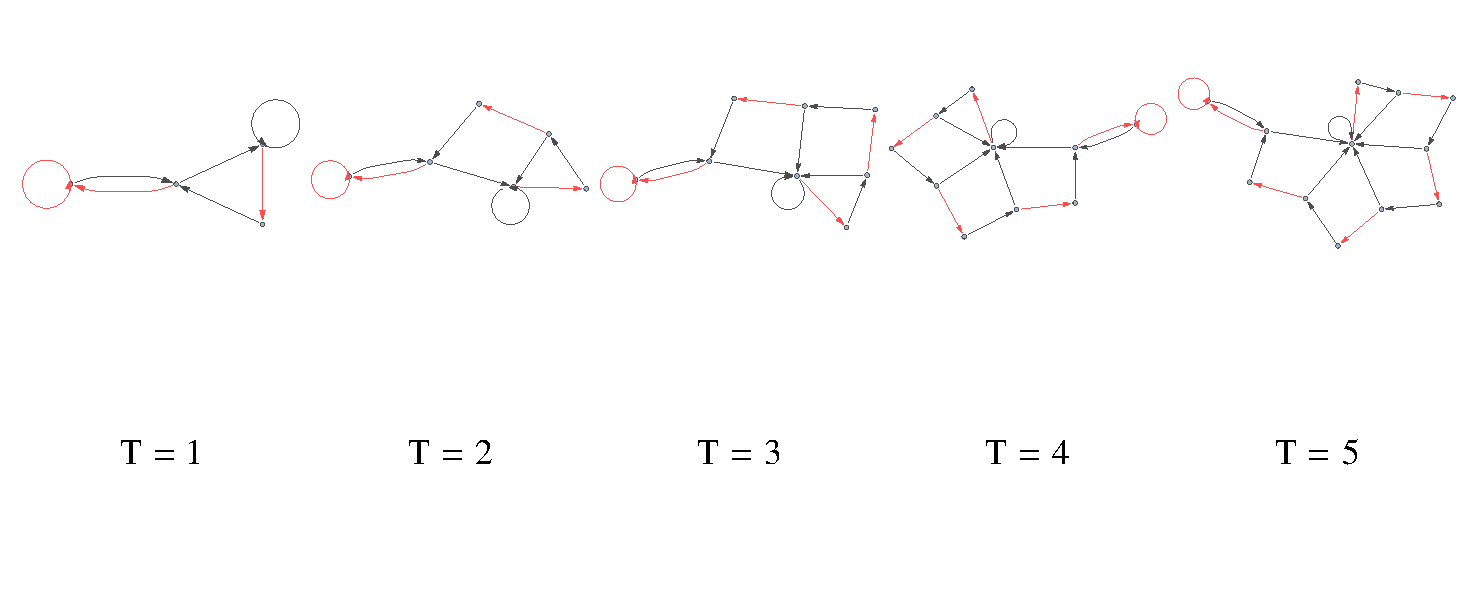
\includegraphics[scale=1]{img/184_5t.eps}
\caption{Semi-autômatos para os cinco primeiros passos de tempo da regra 184}
\label{fig:184-5t}
\end{center}
\end{figure}

Utilizando o método apresentado na Seção \ref{sec:mikialgo}, sua conclusão
foi de que a cada passo de tempo, sempre existia uma mesma estrutura
de grafo sendo adicionada e uma sendo excluída, e essas estruturas eram
invariantes no tempo. As Figuras \ref{fig:addstruct} e \ref{fig:excstruct}
mostram, respectivamente, as estruturas adicionada e excluída dos sucessivos
semi-autômatos.

\begin{figure}[htp]
\begin{minipage}[b]{0.5\linewidth}
\centering
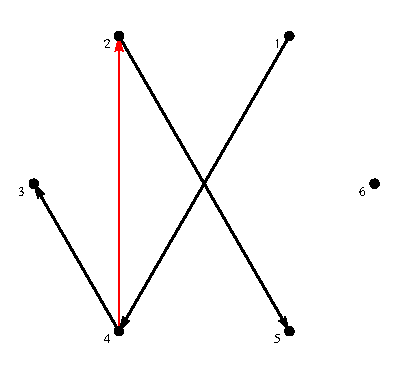
\includegraphics[scale=1]{img/addStruct.eps}
\caption{Estrutura adicionada \citecustom{miki2006}}
\label{fig:addstruct}
\end{minipage}
\hspace{0.5cm}
\begin{minipage}[b]{0.5\linewidth}
\centering
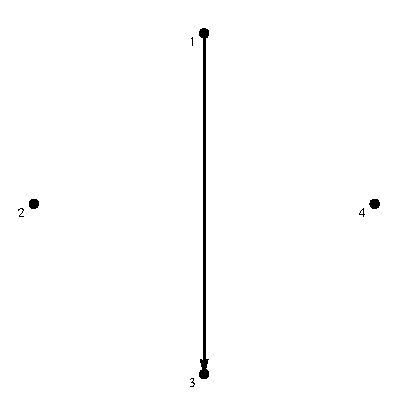
\includegraphics[scale=1]{img/excStruct.eps}
\caption{Estrutura excluída \citecustom{miki2006}}
\label{fig:excstruct}
\end{minipage}
\end{figure}

É difícil identificar visualmente estas estruturas, ou qualquer padrão de
crescimento, por meio dos semi-autômatos. Porém, convertendo estes grafos
em matrizes de adjacências isomórficas, é possível detectar os padrões
de crescimento e visualizar o efeito das estruturas adicionada e
excluída. As Figuras \ref{fig:addstructm} e \ref{fig:excstructm} mostram
as respectivas estruturas adicionada e excluída em notação matricial, e
a Tabela \ref{tab:mr184} mostra a evolução no tempo da regra 184 em notação
de grafo e matricial.

\begin{figure}[htp]
\begin{minipage}[b]{0.5\linewidth}
\begin{center}
\begin{math}
\begin{pmatrix}
0 & 0 & 0 & 2 & 0 & 0 \\
0 & 0 & 0 & 0 & 2 & 0 \\
0 & 0 & 0 & 0 & 0 & 0 \\
0 & 1 & 2 & 0 & 0 & 0 \\
0 & 0 & 0 & 0 & 0 & 0 \\
0 & 0 & 0 & 0 & 0 & 0
\end{pmatrix}
\end{math}
\caption{Estrutura adicionada em notação matricial}
\label{fig:addstructm}
\end{center}
\end{minipage}
\hspace{0.5cm}
\begin{minipage}[b]{0.5\linewidth}
\begin{center}
\begin{math}
\begin{pmatrix}
0 & 0 & 2 & 0 \\
0 & 0 & 0 & 0 \\
0 & 0 & 0 & 0 \\
0 & 0 & 0 & 0
\end{pmatrix}
\end{math}
\caption{Estrutura excluída em notação matricial}
\label{fig:excstructm}
\end{center}
\end{minipage}
\end{figure}

Embora devido à diferença nos tamanhos das matrizes não seja possível
derivar uma operação algébrica, é fácil notar o que acontece na evolução
da regra 184 olhando as matrizes de adjacências da regra e as estruturas
adicionada e excluída.

Observando duas matrizes de tempo $t$ e tempo $t+1$, repara-se que:

\begin{enumerate}
\item Existe uma diagonal de transições em $1$ que começa em $A_{t+1,1}$
e vai até $A_{2t,t}$. A cada passo de tempo, uma transição em $1$ é adicionada,
o que corresponde ao valor $1$ na posição $(4,2)$ da estrutura adicionada.

\item Existe um coluna de transições em $2$ iniciando-se na posição
$A_{t+1,t+1}$ e terminando na posição $A_{N-1,t+1}$. Novamente observa-se
que a cada passo de tempo, uma linha com uma transição em $2$ é adiciona à
coluna, e essa transição corresponde ao valor $2$ na posição $(4,3)$ na matriz da
estrutura adicionada.

\item Uma diagonal de transições em $2$ aparece na posição $A_{1,t+2}$ indo
até a posição $A_{t,N-1}$. Olhando para a matriz da estrutura adicionada,
observa-se que duas transições em $2$ são adicionadas a esta diagonal a cada
passo de tempo, mas uma dessas transições é retirada conforme se nota na
matriz da estrutura excluída.

\item Por fim, uma transição em $1$ é atribuída à posição $A_{N,N}$, uma
outra transição em $1$ na posição $A_{N-1,N}$ e uma transição em $2$ é
atribuída na posição $A_{N,N-1}$.
\end{enumerate}

Baseando-se nesta análise, é possível derivar um algoritmo de construção da
matriz de adjacências isomórfica do semi-autômato de tempo $t$ para a
regra 184. O algoritmo é mostrado no Algoritmo \ref{alg:r184}.

\begin{algorithm}
\caption{Algoritmo para gerar a matriz de adjacências isomórfica do
semi-autômato de tempo $t$ para a regra 184}
\label{alg:r184}
\begin{algorithmic}
\STATE $i \leftarrow t+1$
\FOR{$j=1$ to t}
\STATE $A_{ij} \leftarrow 1$
\STATE $i \leftarrow i+1$
\ENDFOR
\FOR{$i=t+1$ to $(2t+1)$}
\STATE $A_{i,t+1} \leftarrow 2$
\ENDFOR
\STATE $j \leftarrow t+2$
\FOR{$i=1$ to $t$}
\STATE $A_{ij} \leftarrow 2$
\STATE $j \leftarrow j+1$
\ENDFOR
\STATE $A_{N,N} \leftarrow 1$
\STATE $A_{N-1,N} \leftarrow 1$
\STATE $A_{N,N-1} \leftarrow 2$
\end{algorithmic}
\end{algorithm}

De posse deste algoritmo e do Algoritmo \ref{alg:mtos} é possível, então,
recriar o semi-autômato de tempo $t$ para a regra 184.

\subsection{Padrão de formação das matrizes de adjacências isomórficas}

Após um estudo aprofundado e dedução do algoritmo de formação das matrizes
de adjacências isomórficas para a regra 184 descrito na Seção \ref{sec:184},
estudou-se o padrão de formação para todas as mesmas 26 regras estudadas em
\citecustom{mikietal2011}. Conforme mostrado na Tabela \ref{tab:pattern},
todas as regras apresentam um padrão de formação, embora nem sempre a
partir do primeiro instante de tempo. 

\begin{table}[htp]
\begin{center}
\begin{tabular}{|c|c|}
\hline
\textbf{Regra} & \textbf{Padrão de formação} \\ \hline
 11 & Apresenta um padrão de formação intercalado a partir de $t=2$ \\ \hline
 14 & Apresenta um padrão de formação intercalado a partir de $t=2$ \\ \hline
 35 & Apresenta um padrão de formação intercalado a partir de $t=2$ \\ \hline
 43 & Apresenta um padrão de formação a partir de $t=1$ \\ \hline
 50 & Apresenta um padrão de formação intercalado a partir de $t=4$ \\ \hline
 56 & Apresenta um padrão de formação a partir de $t=2$ \\ \hline
 70 & Apresenta um padrão de formação a partir de $t=3$ \\ \hline
 81 & Apresenta um padrão de formação intercalado a partir de $t=3$ \\ \hline
 98 & Apresenta um padrão de formação a partir de $t=2$ \\ \hline
113 & Apresenta um padrão de formação a partir de $t=2$ \\ \hline
128 & Apresenta um padrão de formação a partir de $t=1$ \\ \hline
132 & Apresenta um padrão de formação a partir de $t=2$ \\ \hline
136 & Apresenta um padrão de formação a partir de $t=2$ \\ \hline
140 & Apresenta um padrão de formação a partir de $t=2$ \\ \hline
142 & Apresenta um padrão de formação a partir de $t=2$ \\ \hline
162 & Apresenta um padrão de formação a partir de $t=1$ \\ \hline
168 & Apresenta um padrão de formação a partir de $t=1$ \\ \hline
172 & Apresenta um padrão de formação a partir de $t=2$ \\ \hline
176 & Apresenta um padrão de formação a partir de $t=2$ \\ \hline
184 & Apresenta um padrão de formação a partir de $t=1$ \\ \hline
192 & Apresenta um padrão de formação a partir de $t=2$ \\ \hline
196 & Apresenta um padrão de formação a partir de $t=1$ \\ \hline
212 & Apresenta um padrão de formação a partir de $t=1$ \\ \hline
224 & Apresenta um padrão de formação a partir de $t=2$ \\ \hline
252 & Apresenta um padrão de formação a partir de $t=2$ \\ \hline
\end{tabular}
\caption{Padrão de formação de matrizes de adjacências isomórficas das
regras elementares}
\label{tab:pattern}
\end{center}
\end{table}

Por \textit{padrão de formação} entende-se por uma estrutura presente em $t$ que
pode ser vista em $t+1$ de forma expandida ou contraída. Um \textit{padrão de
formação intercalado} significa que existe um aumento no número de estados
em passos de tempo adjacentes ($t$ e $t+1$), mas o aumento de transições só se
da a cada dois passos de tempo ($t$ e $t+2$).

A partir da Tabela \ref{tab:pattern}, conclui-se que as regras estão divididas
em dois grupos base: as que apresentam um padrão a partir de $t=n$ e as que
apresentam um padrão intercalado a partir de $t=n,\exists n \in \mathbb{N}$.
A análise baseou-se a partir da observação dos cinco primeiros passos de
tempo e, quando o padrão de formação se deu a partir de $t=4$, analisou-se
os dez primeiros passos de tempo. O Apêndice \ref{sec:matrices} mostra as
matrizes analisadas. Observe que algumas matrizes são parcialmente mostradas
porque são muito grandes para caber na tabela.

\section{Conclusão}\label{sec:conclude}

Autômatos celulares são sistemas discretos no espaço e no tempo que
possuem comportamento local simples e determinístico mas que podem possuir
comportamento global extremamente complexo. O conjunto de configurações
globais que podem ser vistas em um autômato celular após um determinado
número de passos de evolução pode ser descrito por uma linguagem
regular. Linguagem regulares são um conjunto de cadeias formadas
por um alfabeto dentro da linguagem.

Este trabalho trata-se do estudo da complexidade de um subconjunto de autômatos
celulares elementares. O objetivo é dar continuidade aos trabalhos de
\citeonline{trafaniuc2004} e \citeonline{miki2006}. Nestes trabalhos, foi feita
uma profunda análise dos semi-autômatos dos diferentes passos de tempo
para as regras elementares.

Aqui, a abordagem utilizada foi a de converter os semi-autômatos dos sucessivos
passos de tempo das regras do espaço elementar em matrizes de adjacências e analisar
tais matrizes. Porém, a notação comumente utilizada para matrizes de adjacências
não consegue completamente descrever os semi-autômatos. Foi, então, proposta uma
nova notação de matrizes de adjacências, chamada de \textit{matrizes de
adjacências isomórficas}, assim chamadas porque existe um isomorfismo entre
o semi-autômato e sua respectiva matriz de adjacências. Com isso, foi possível
construir o semi-autômato a partir de sua matriz de adjacências isomórfica.

Depois, mostrou-se que é possível deduzir um algoritmo para o semi-autômato
de tempo $t$ baseado na análise das respectivas matrizes de adjacências e tal
algoritmo foi deduzido para a regra 184. Após, foi feita então uma análise 
dos padrões de evolução das matrizes para as 26 regras estudadas em
\citecustom{mikietal2011}.

Conclui-se então que a nova notação de matrizes de adjacências proposta
pode melhor representar um semi-autômato para caracterização da complexidade
de autômatos celulares elementares, e que a relação de isomorfismo entre
a matriz e seu semi-autômato torna possível a obtenção do algoritmo de
geração do semi-autômato de tempo $t$ a um custo computacional muito
menor em relação a abordagem de geração de semi-autômatos sucessivos.

\newpage

\appendix
\section{Tabelas de evolução das regras do espaço elementar}\label{sec:matrices}

\newpage

\begin{table}[H]
\begin{center}
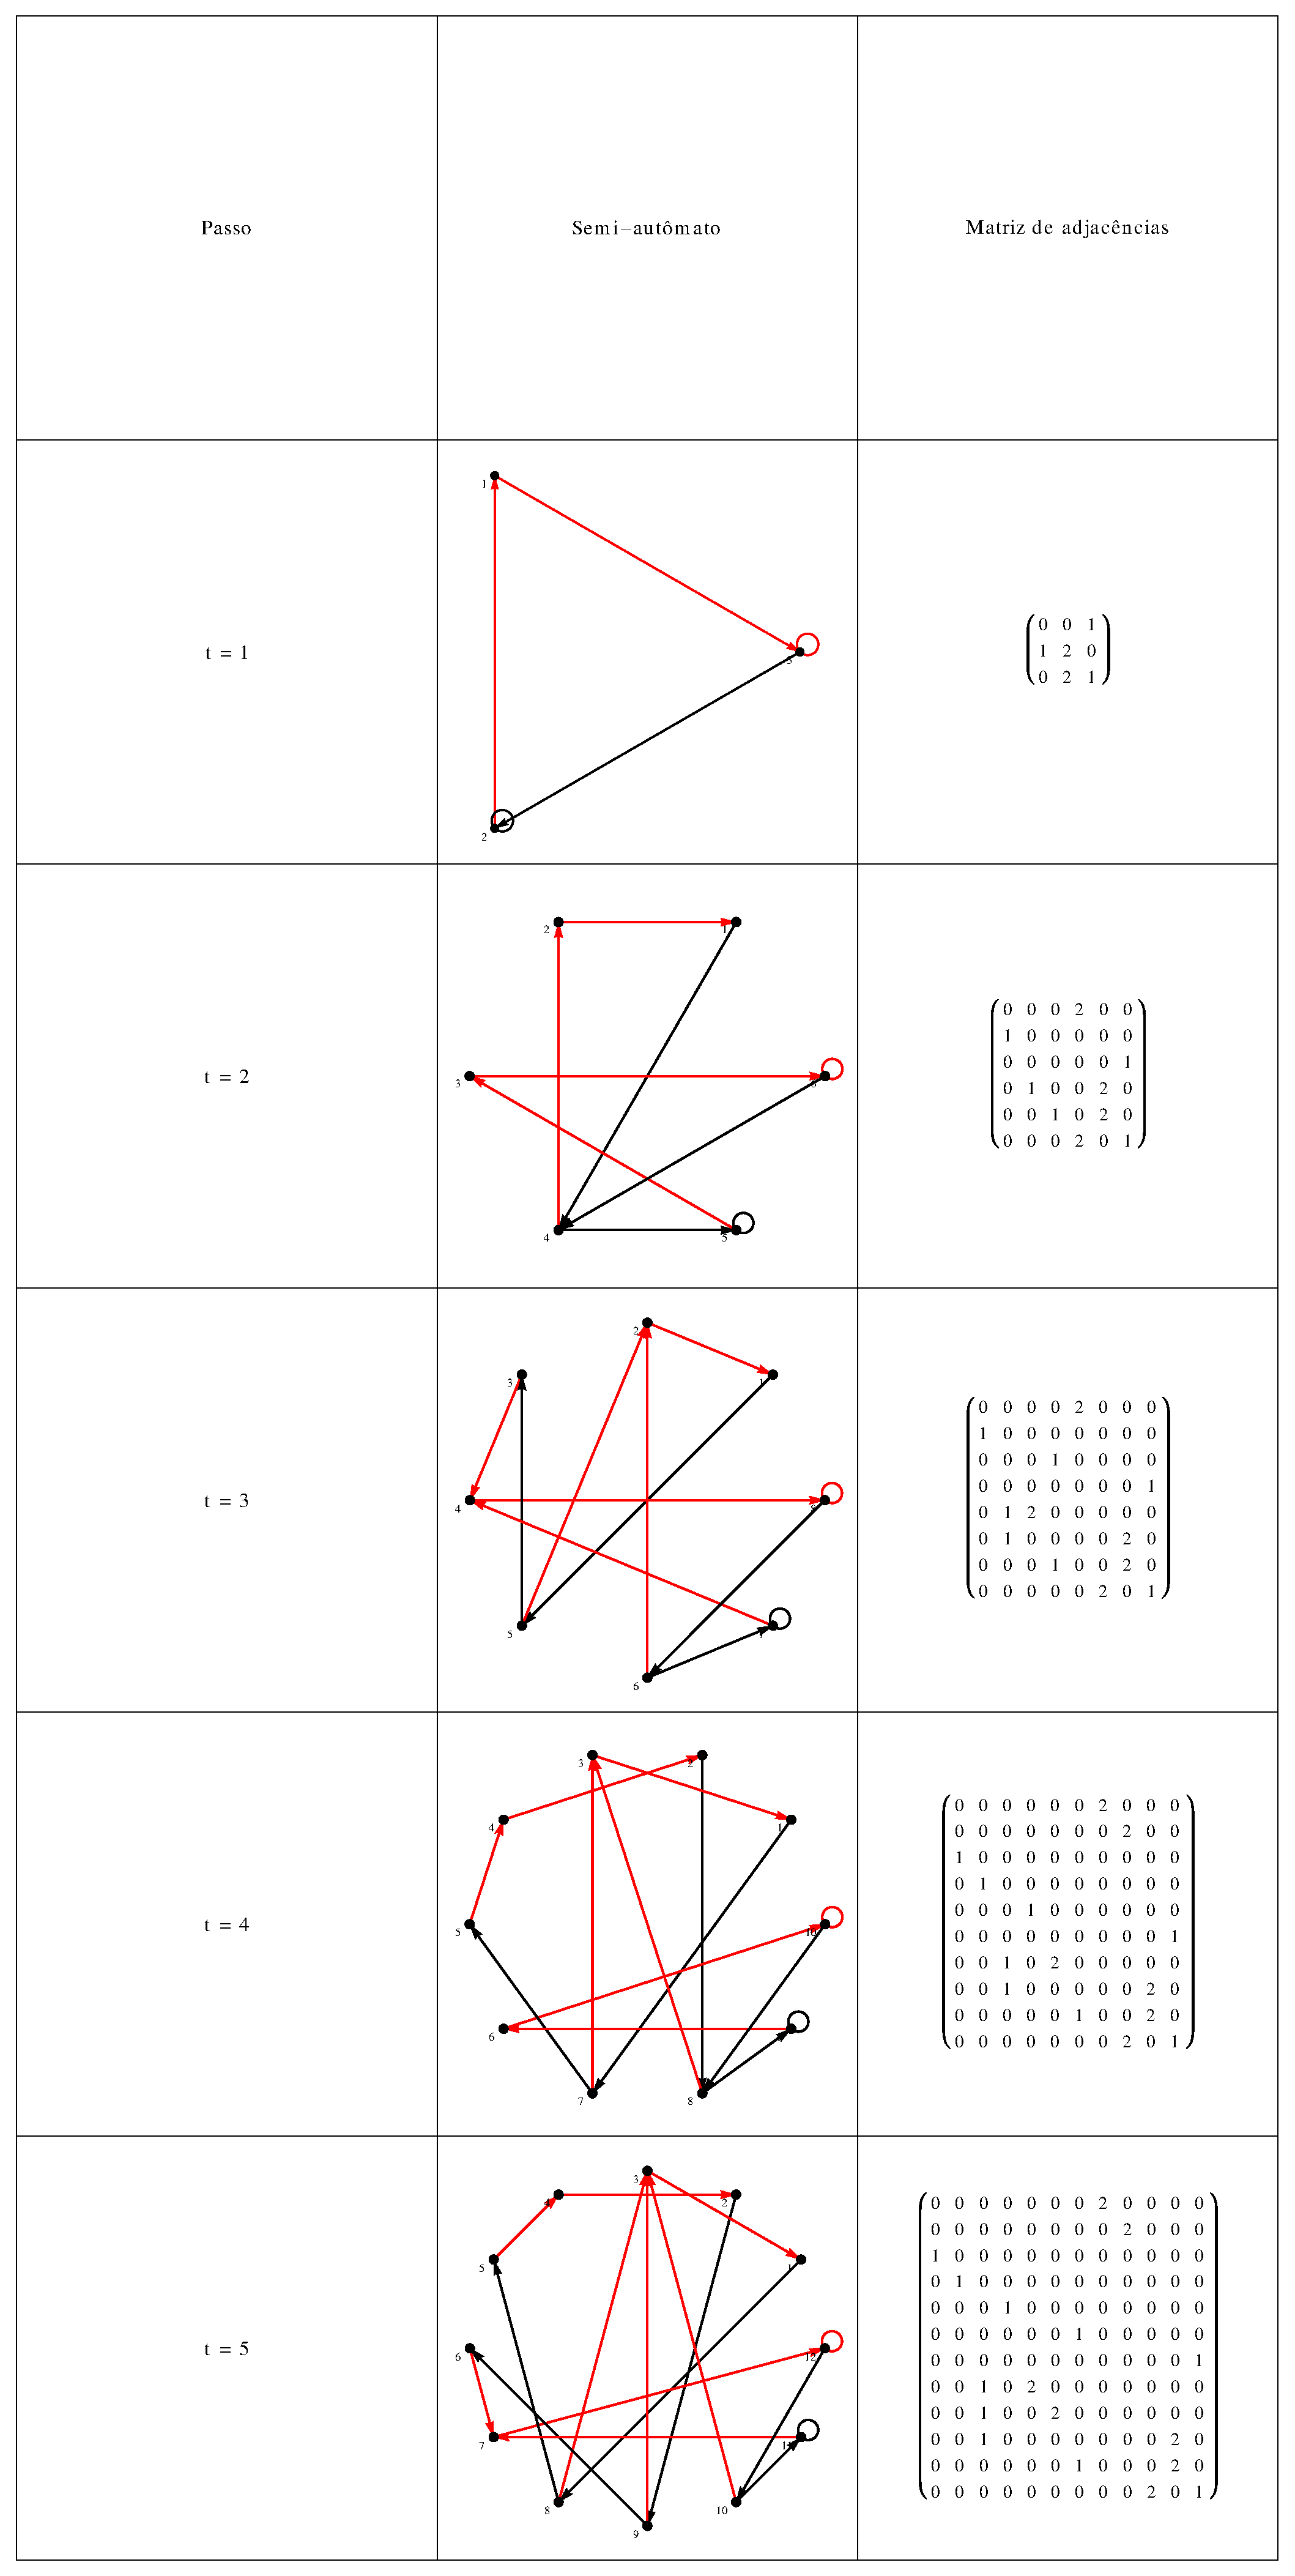
\includegraphics[scale=0.32]{img/mat/matr11.eps}
\caption{Regra 11.}
\label{tab:mr11}
\end{center}
\end{table}

\begin{table}[H]
\begin{center}
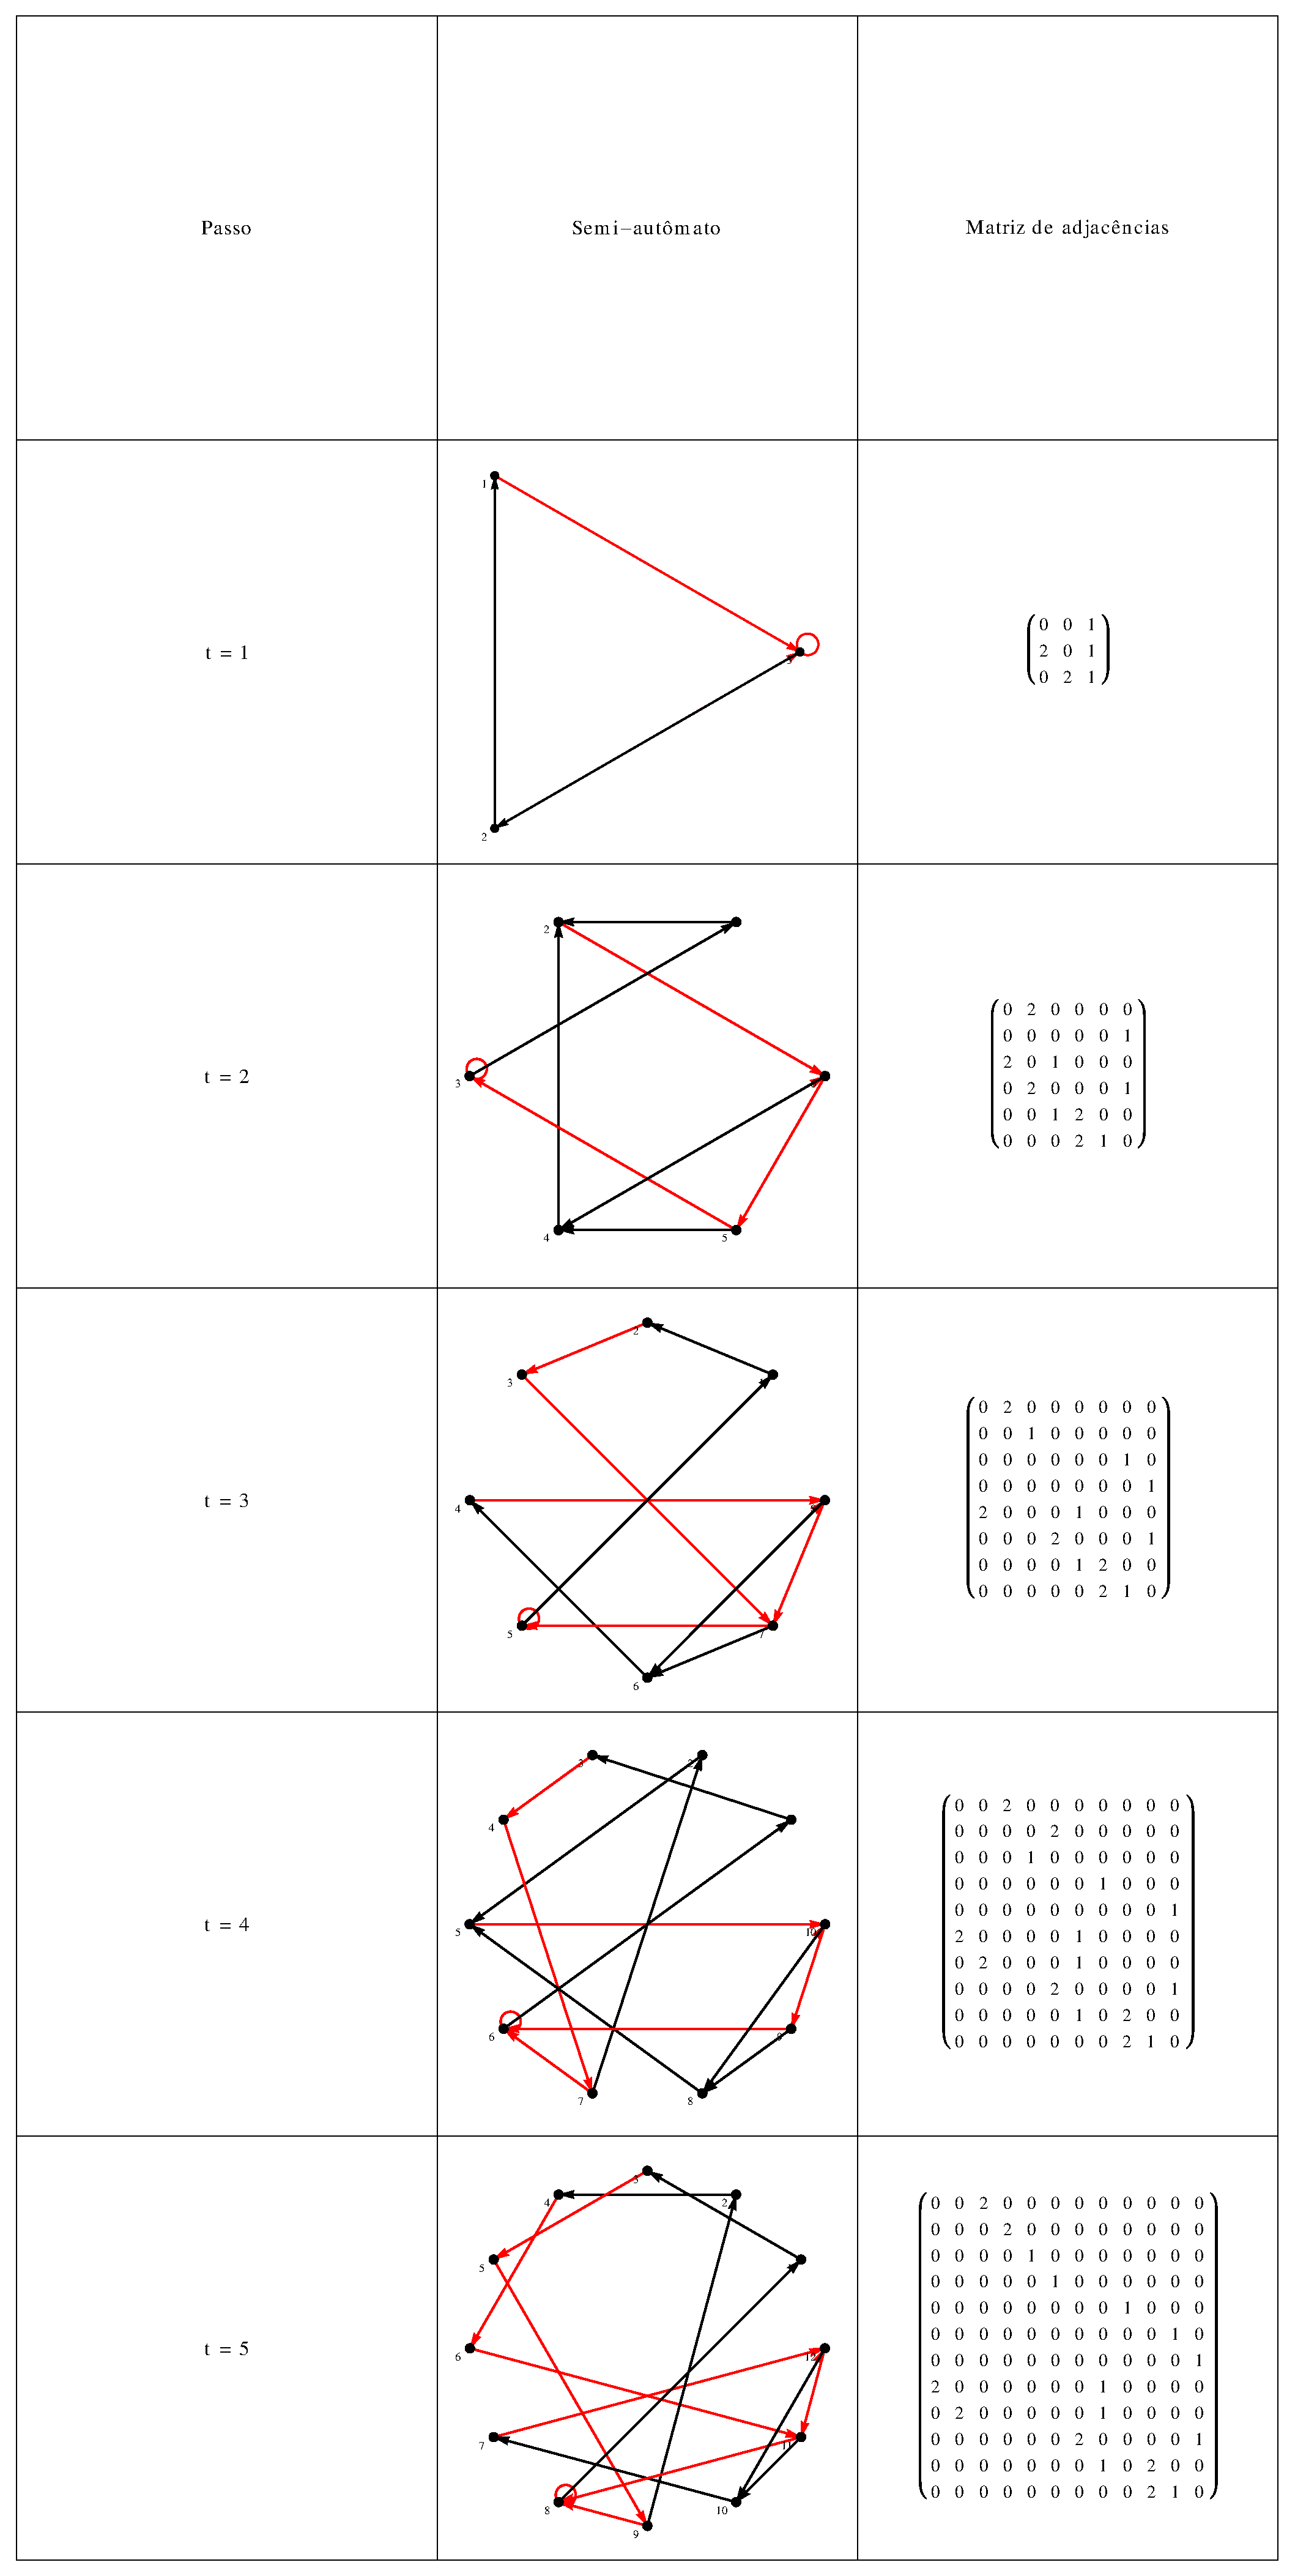
\includegraphics[scale=0.32]{img/mat/matr14.eps}
\caption{Regra 14.}
\label{tab:mr14}
\end{center}
\end{table}

\begin{table}[H]
\begin{center}
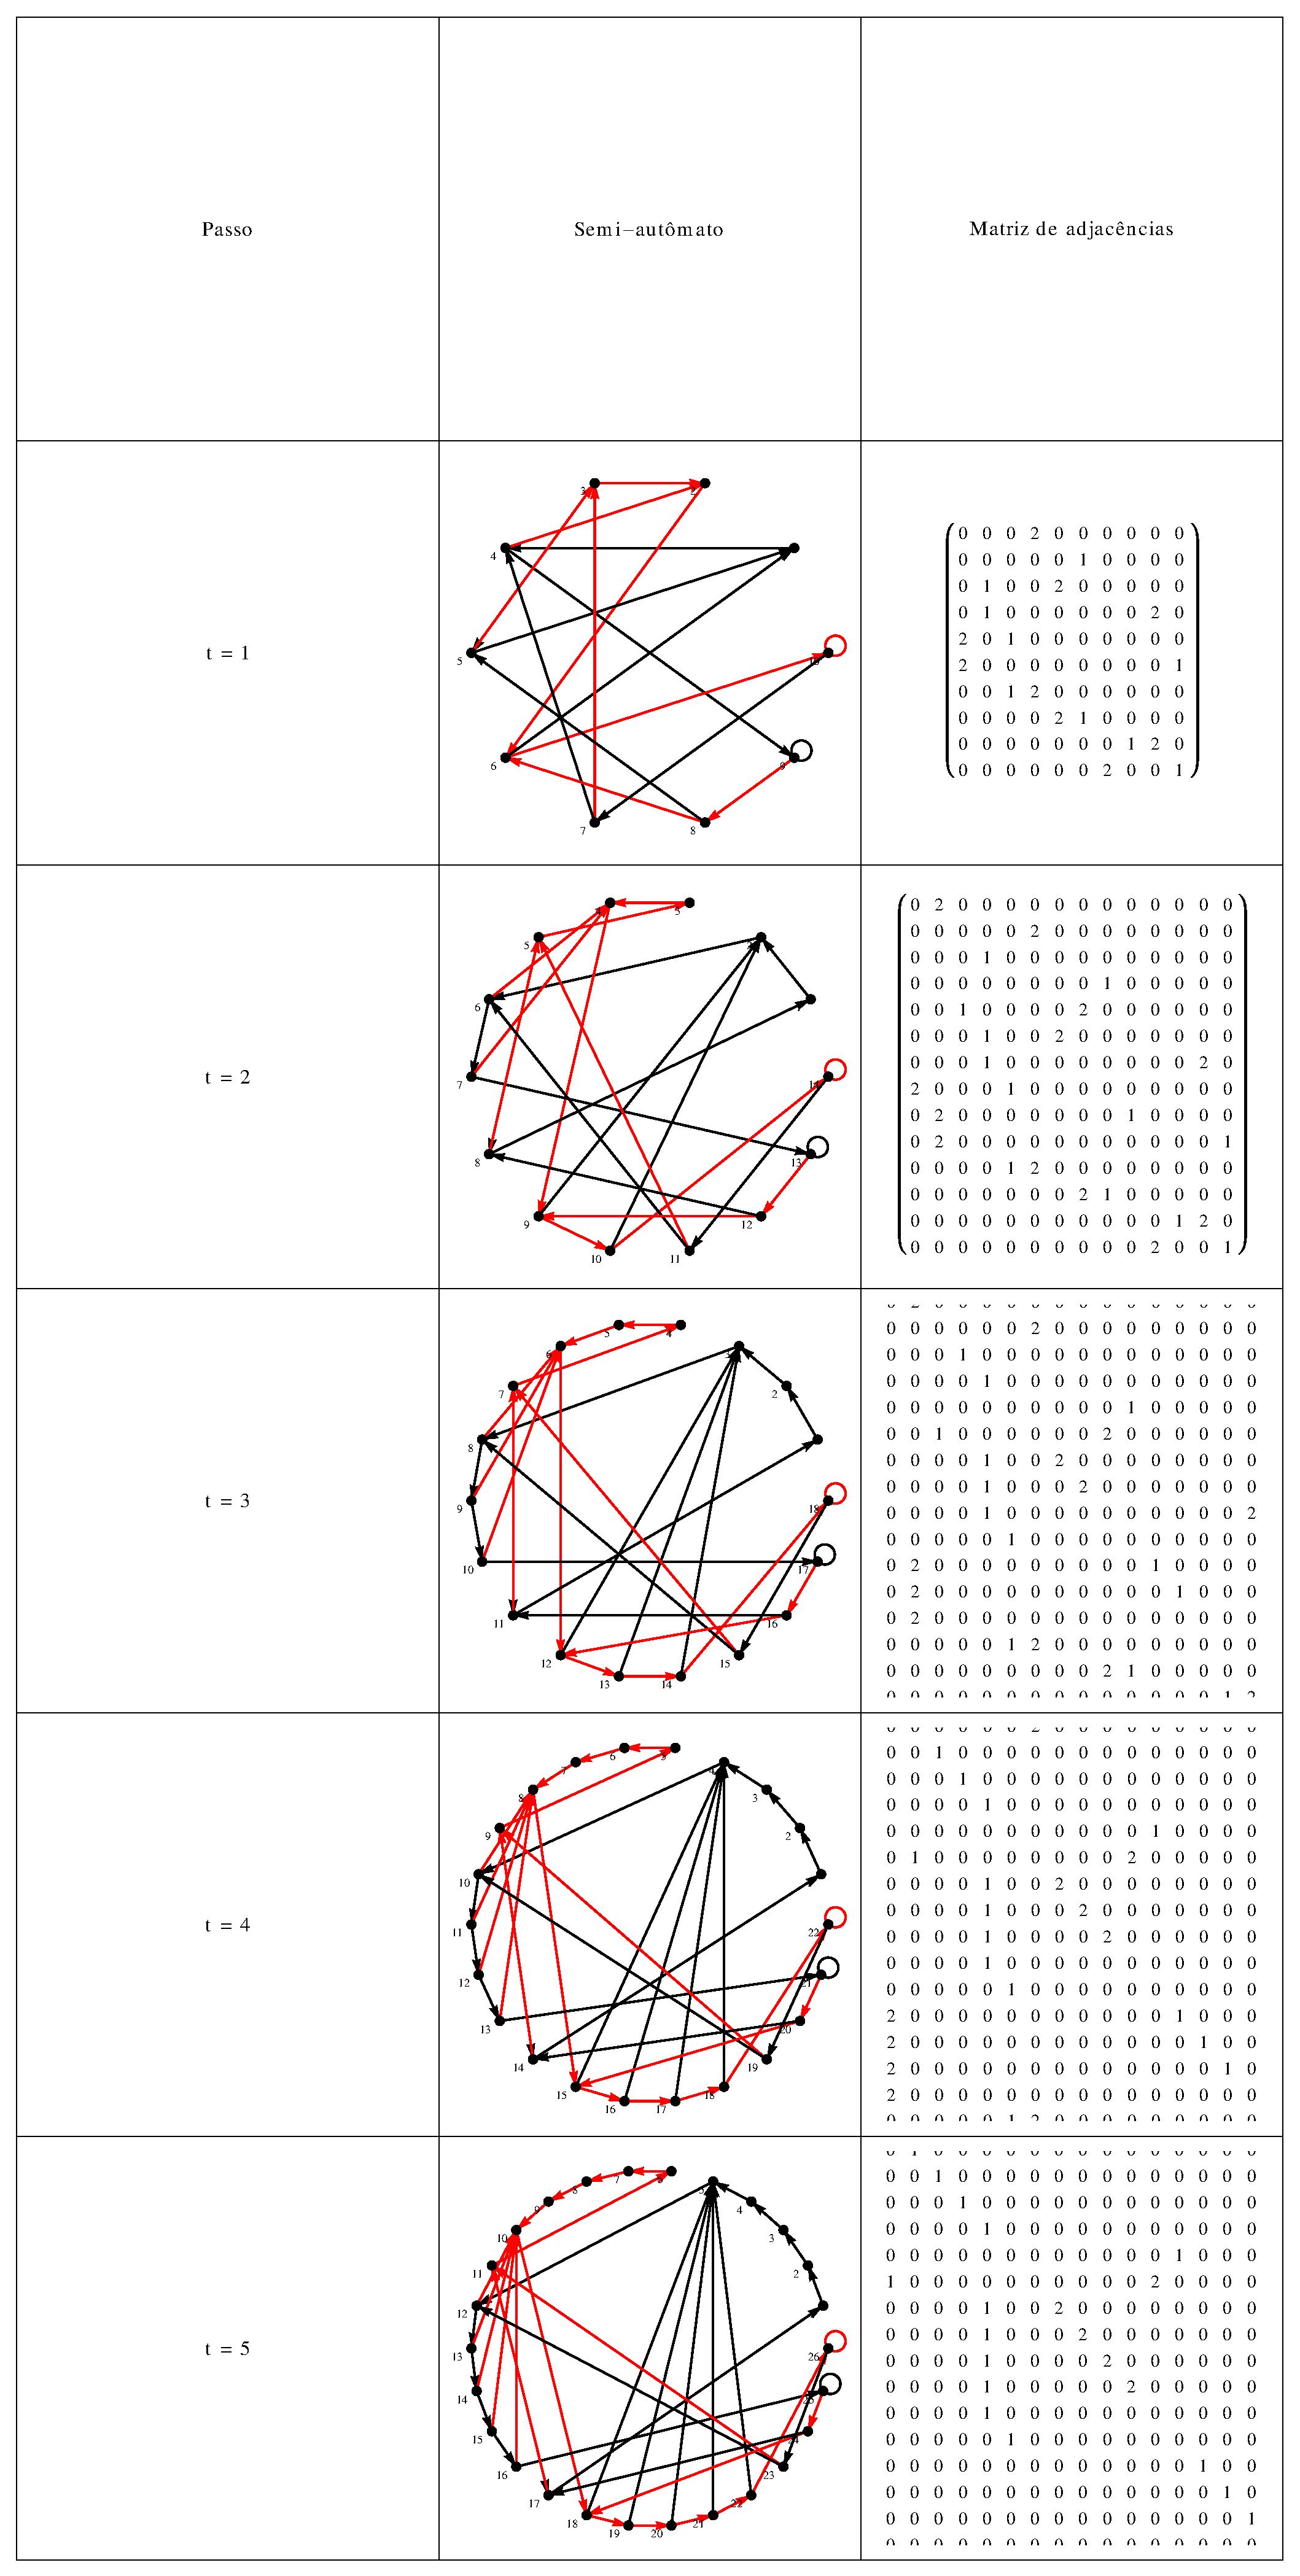
\includegraphics[scale=0.32]{img/mat/matr23.eps}
\caption{Regra 23.}
\label{tab:mr23}
\end{center}
\end{table}

\begin{table}[H]
\begin{center}
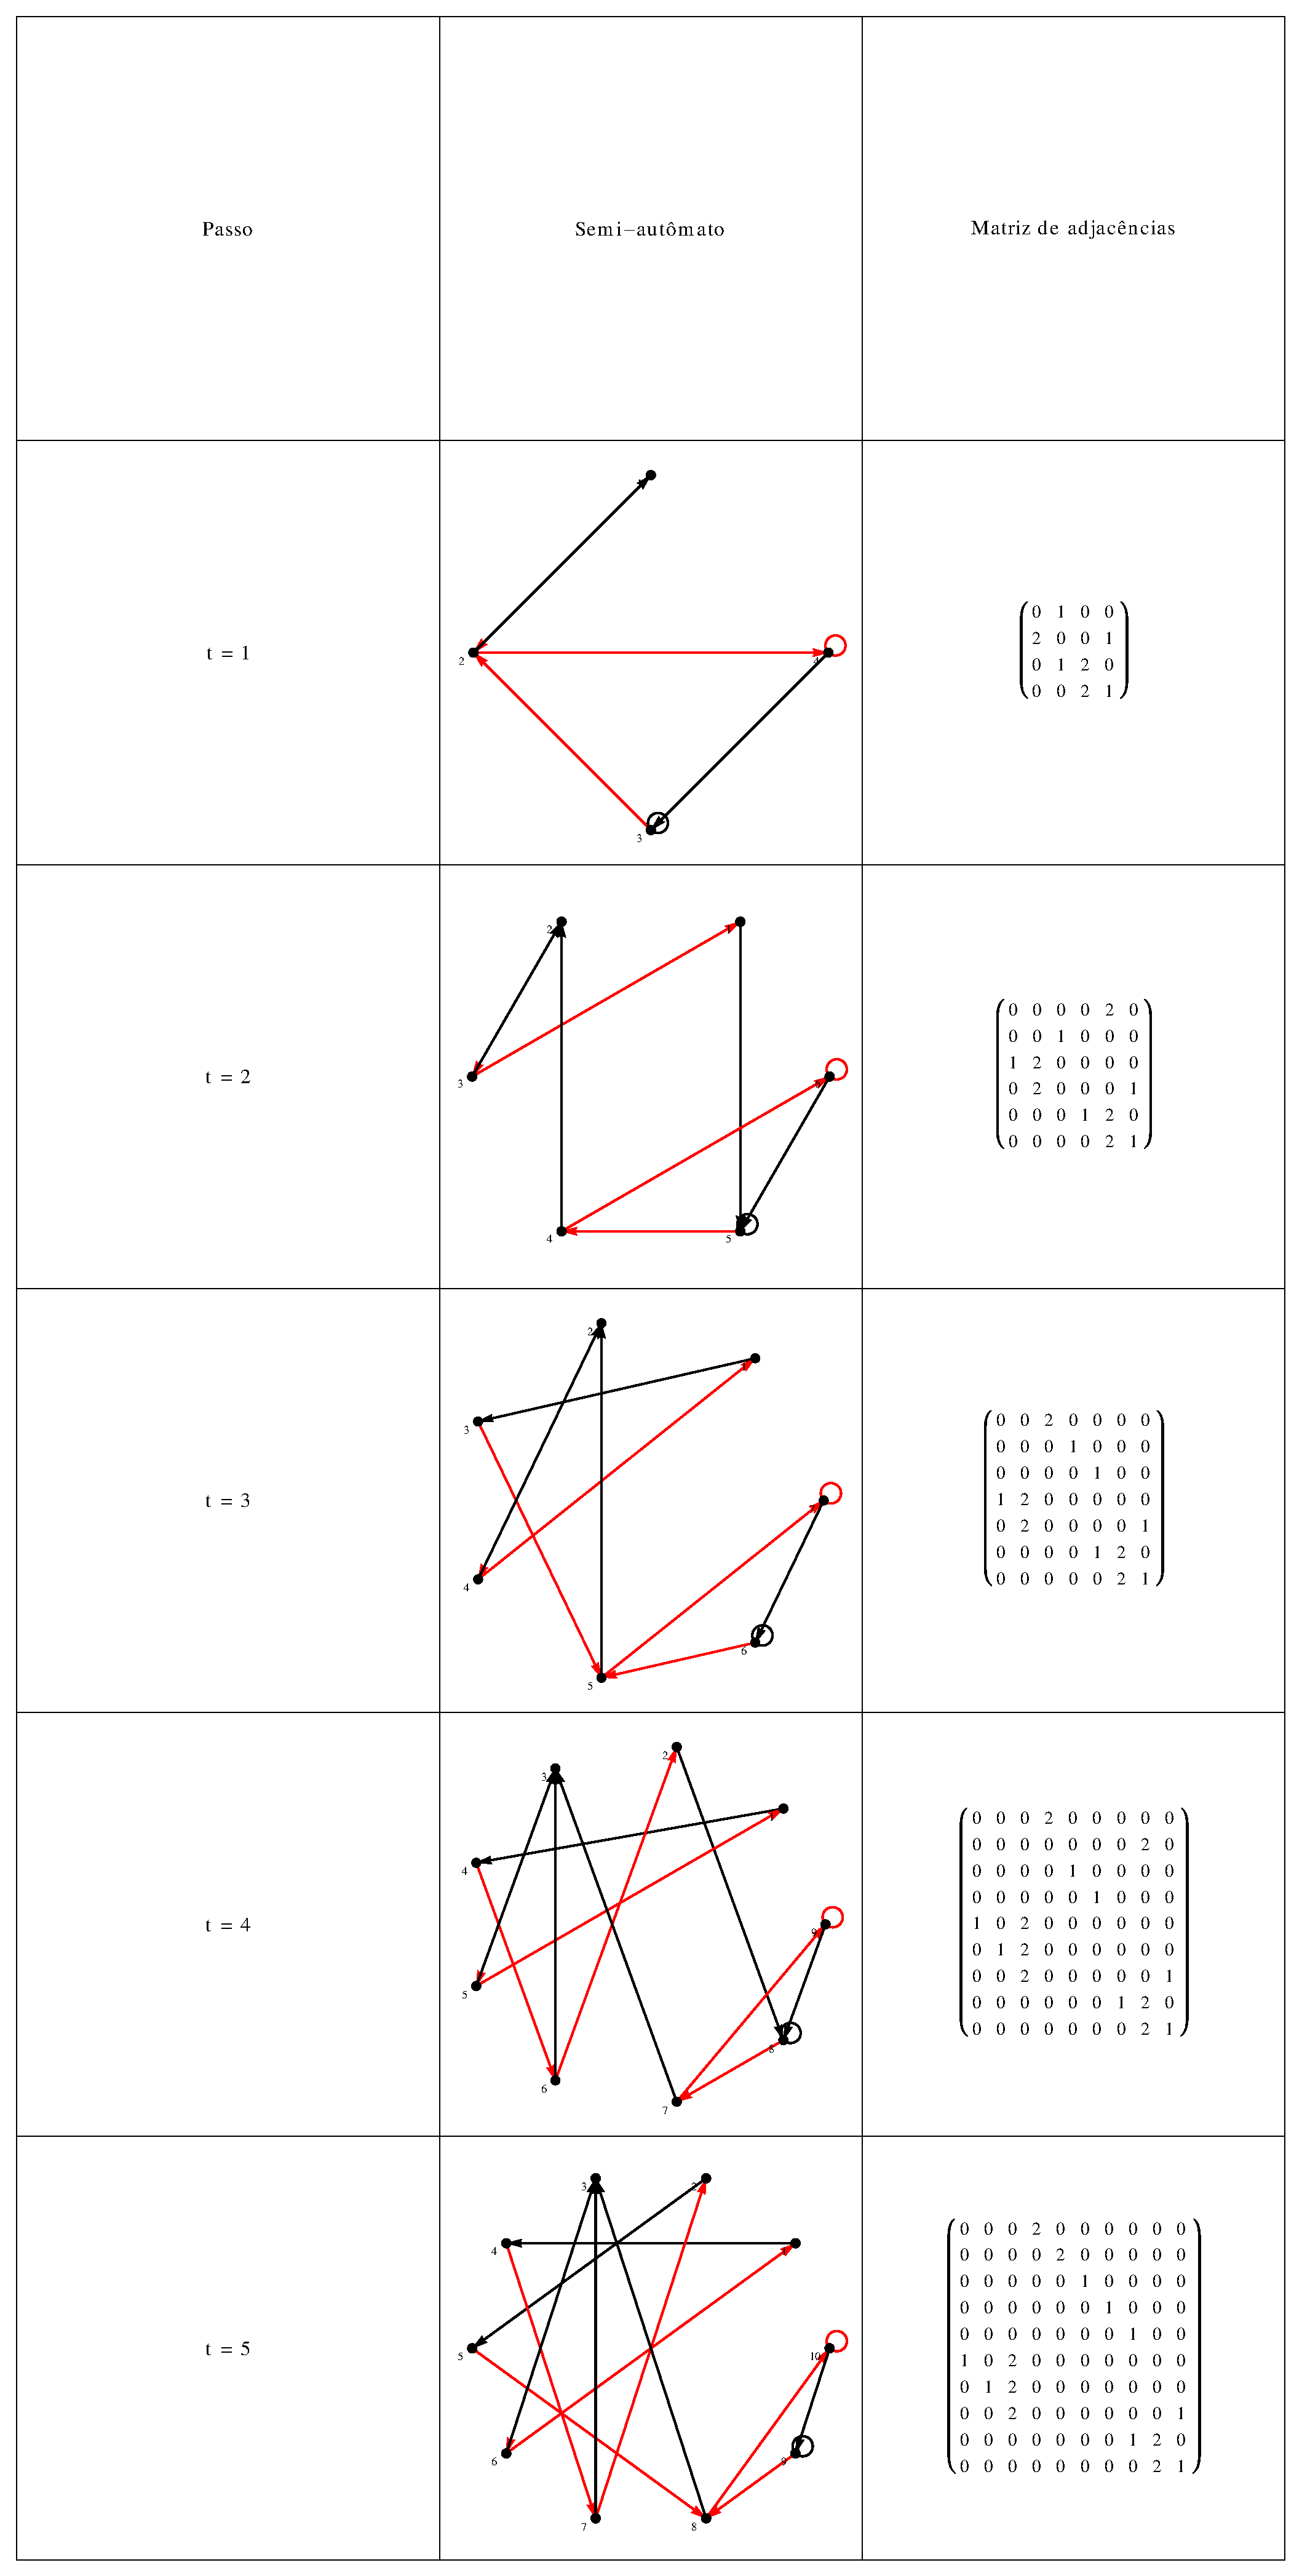
\includegraphics[scale=0.32]{img/mat/matr35.eps}
\caption{Regra 35.}
\label{tab:mr35}
\end{center}
\end{table}

\begin{table}[H]
\begin{center}
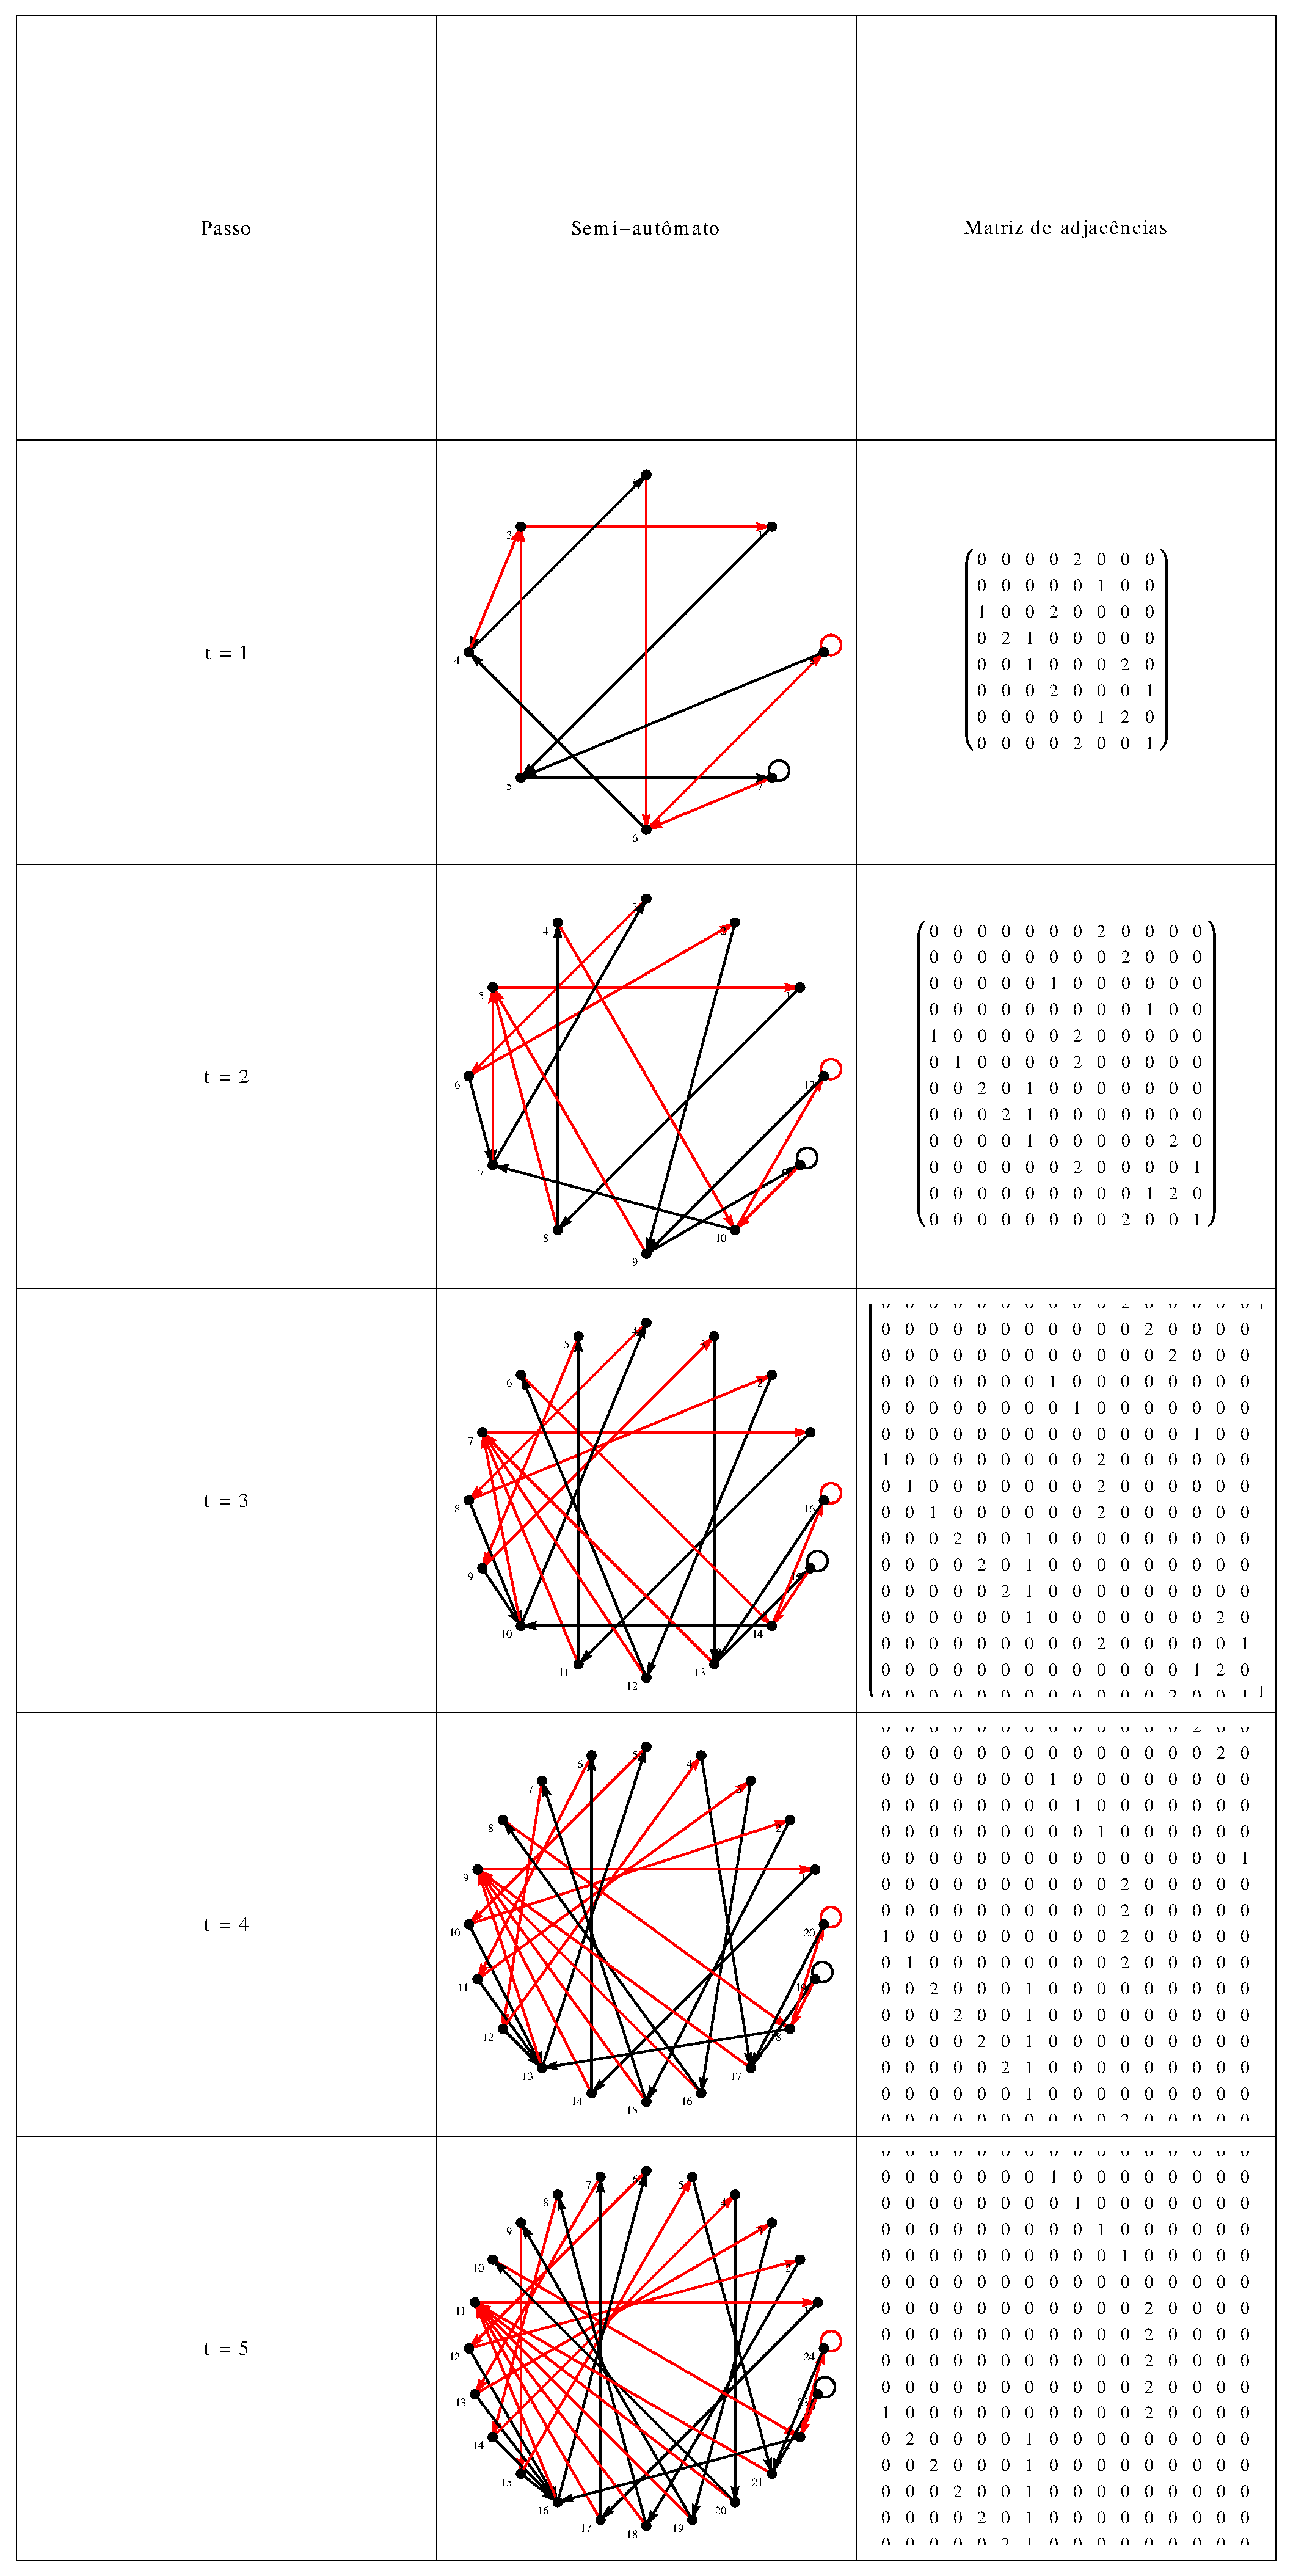
\includegraphics[scale=0.32]{img/mat/matr43.eps}
\caption{Regra 43.}
\label{tab:mr43}
\end{center}
\end{table}

\begin{table}[H]
\begin{center}
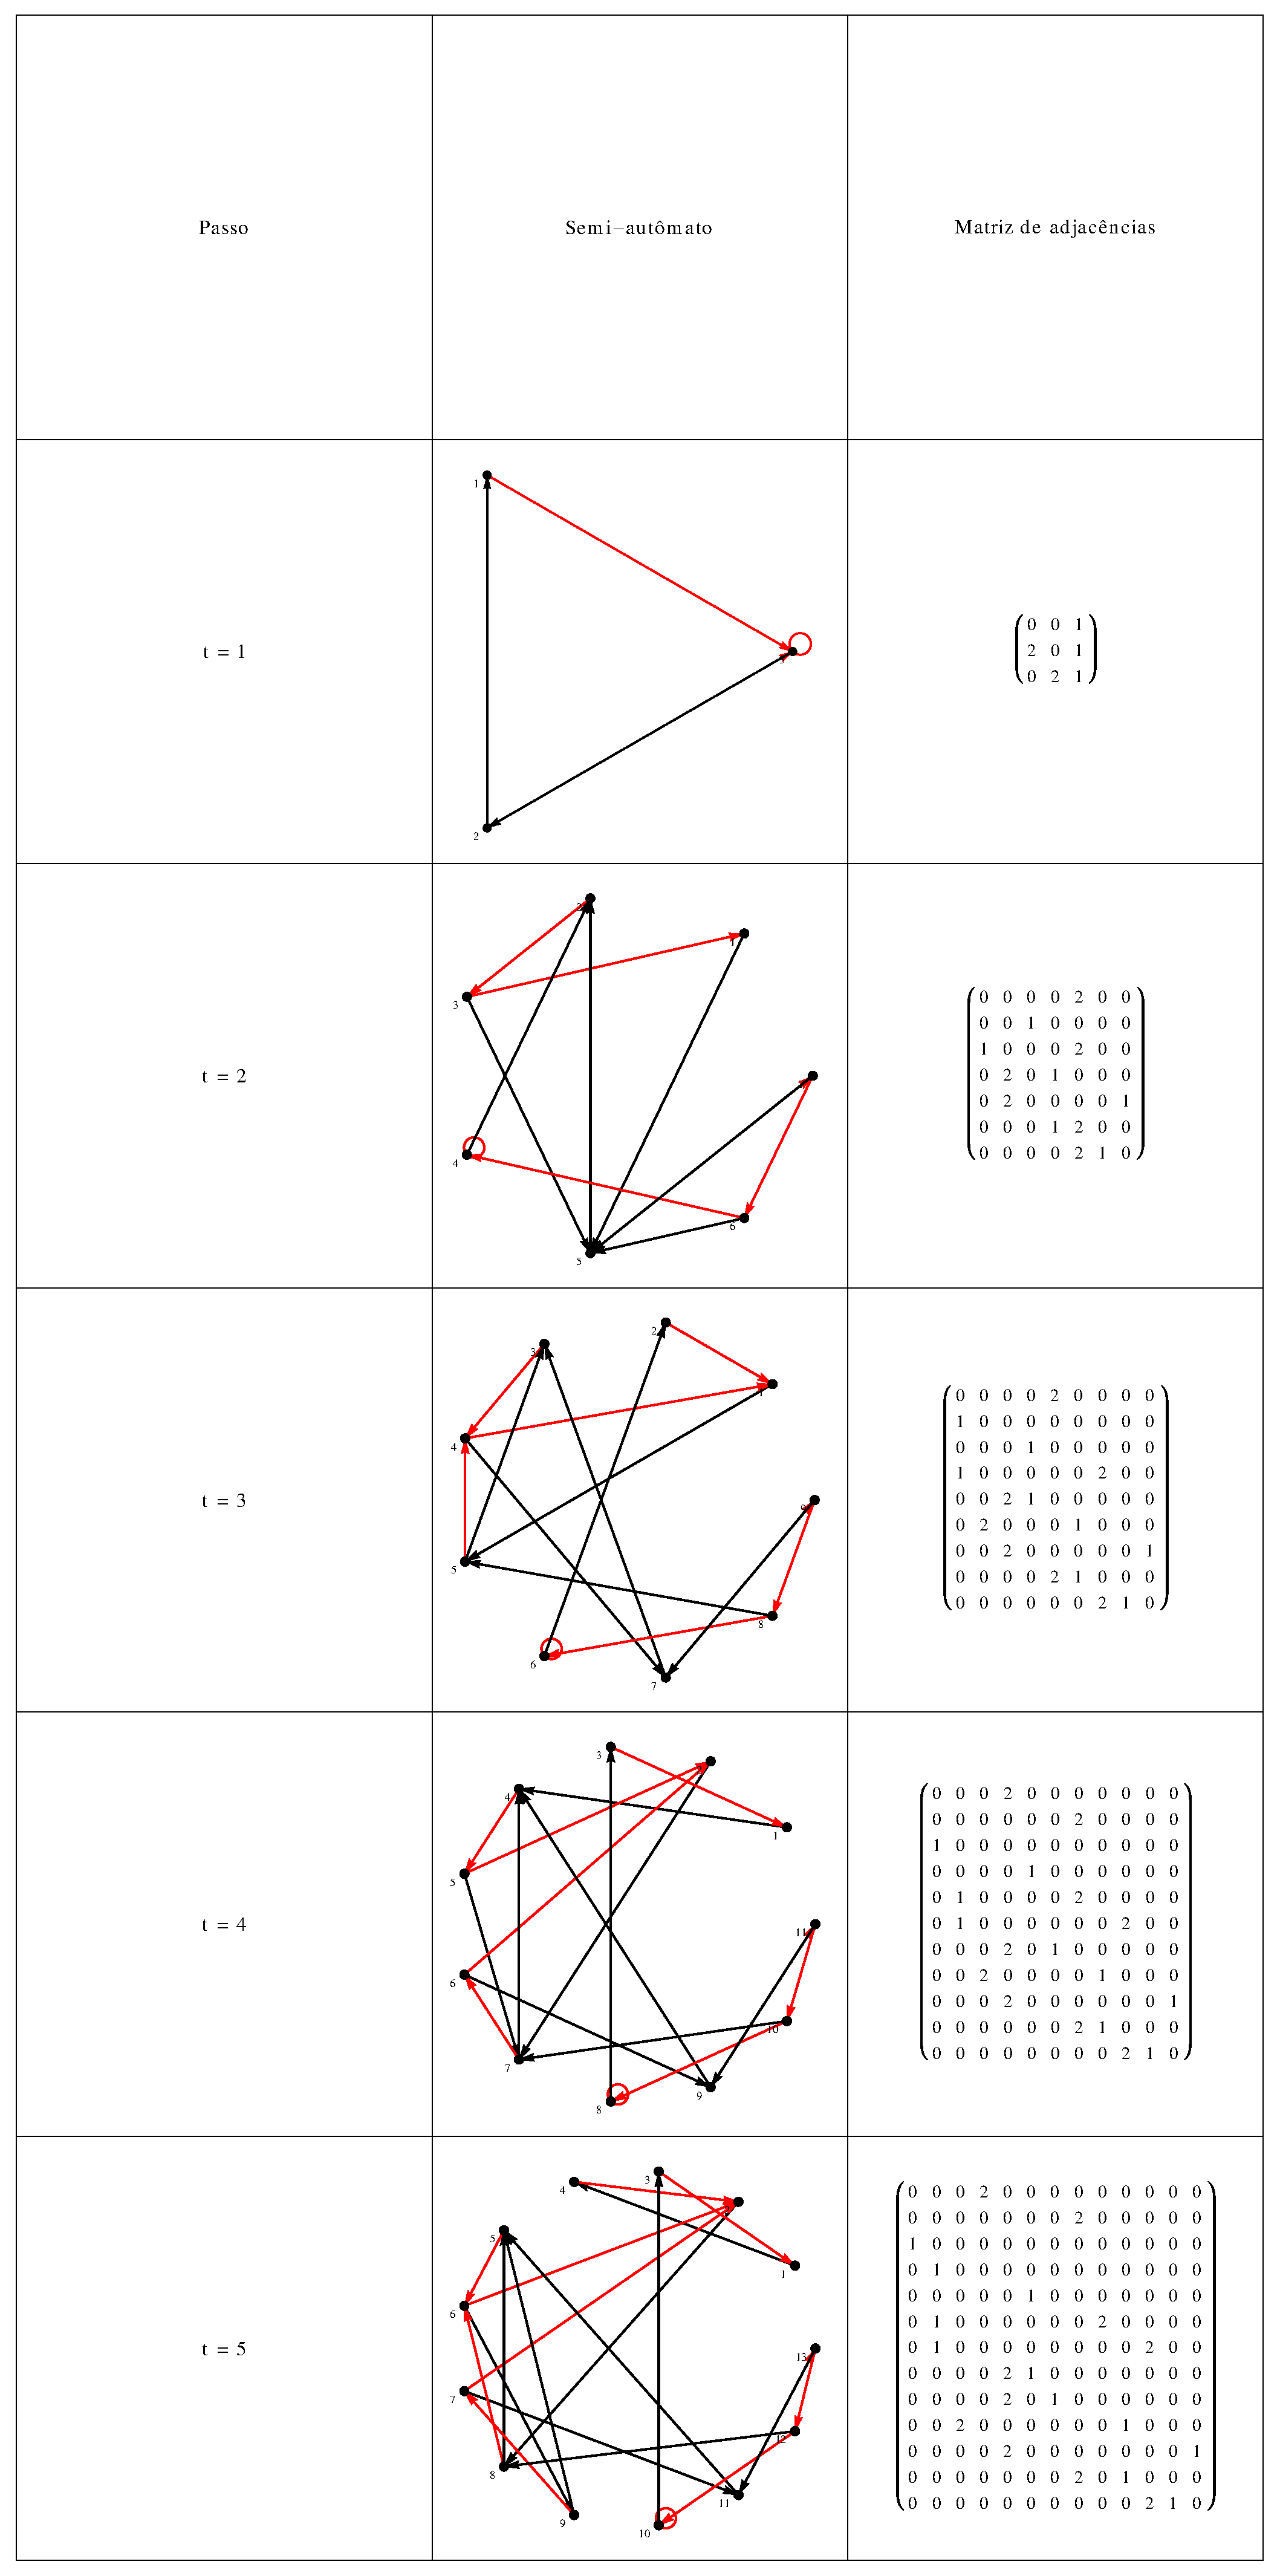
\includegraphics[scale=0.32]{img/mat/matr50.eps}
\caption{Regra 50.}
\label{tab:mr50}
\end{center}
\end{table}

\begin{table}[H]
\begin{center}
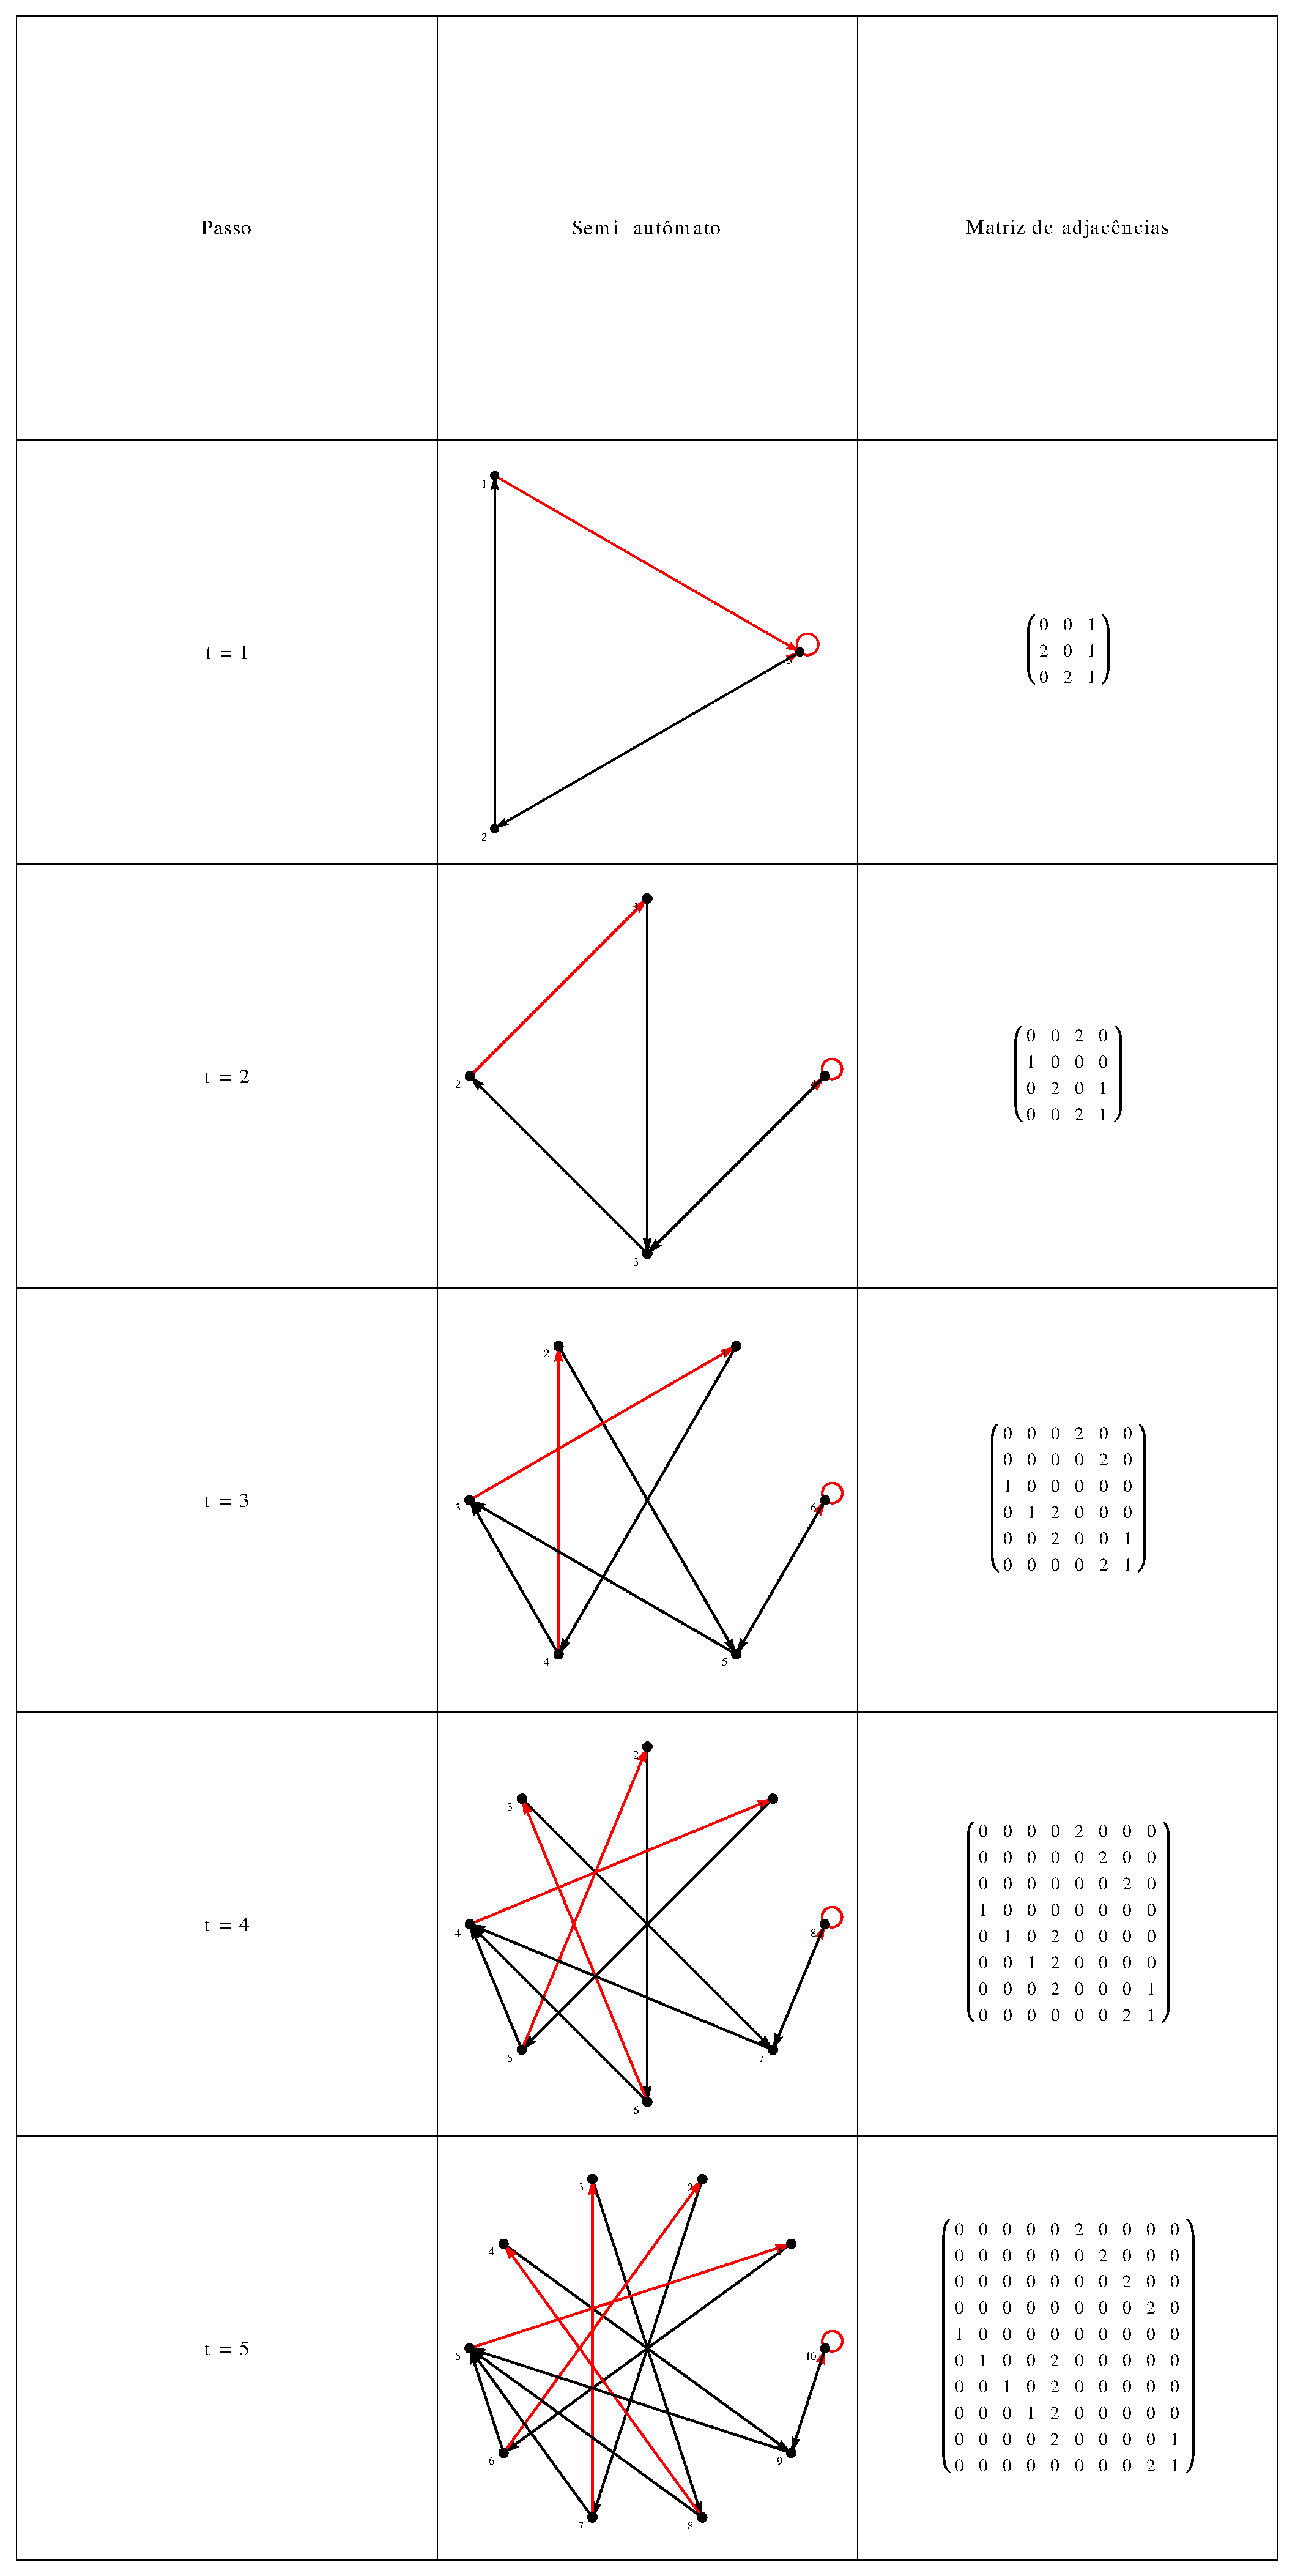
\includegraphics[scale=0.32]{img/mat/matr56.eps}
\caption{Regra 56.}
\label{tab:mr56}
\end{center}
\end{table}

\begin{table}[H]
\begin{center}
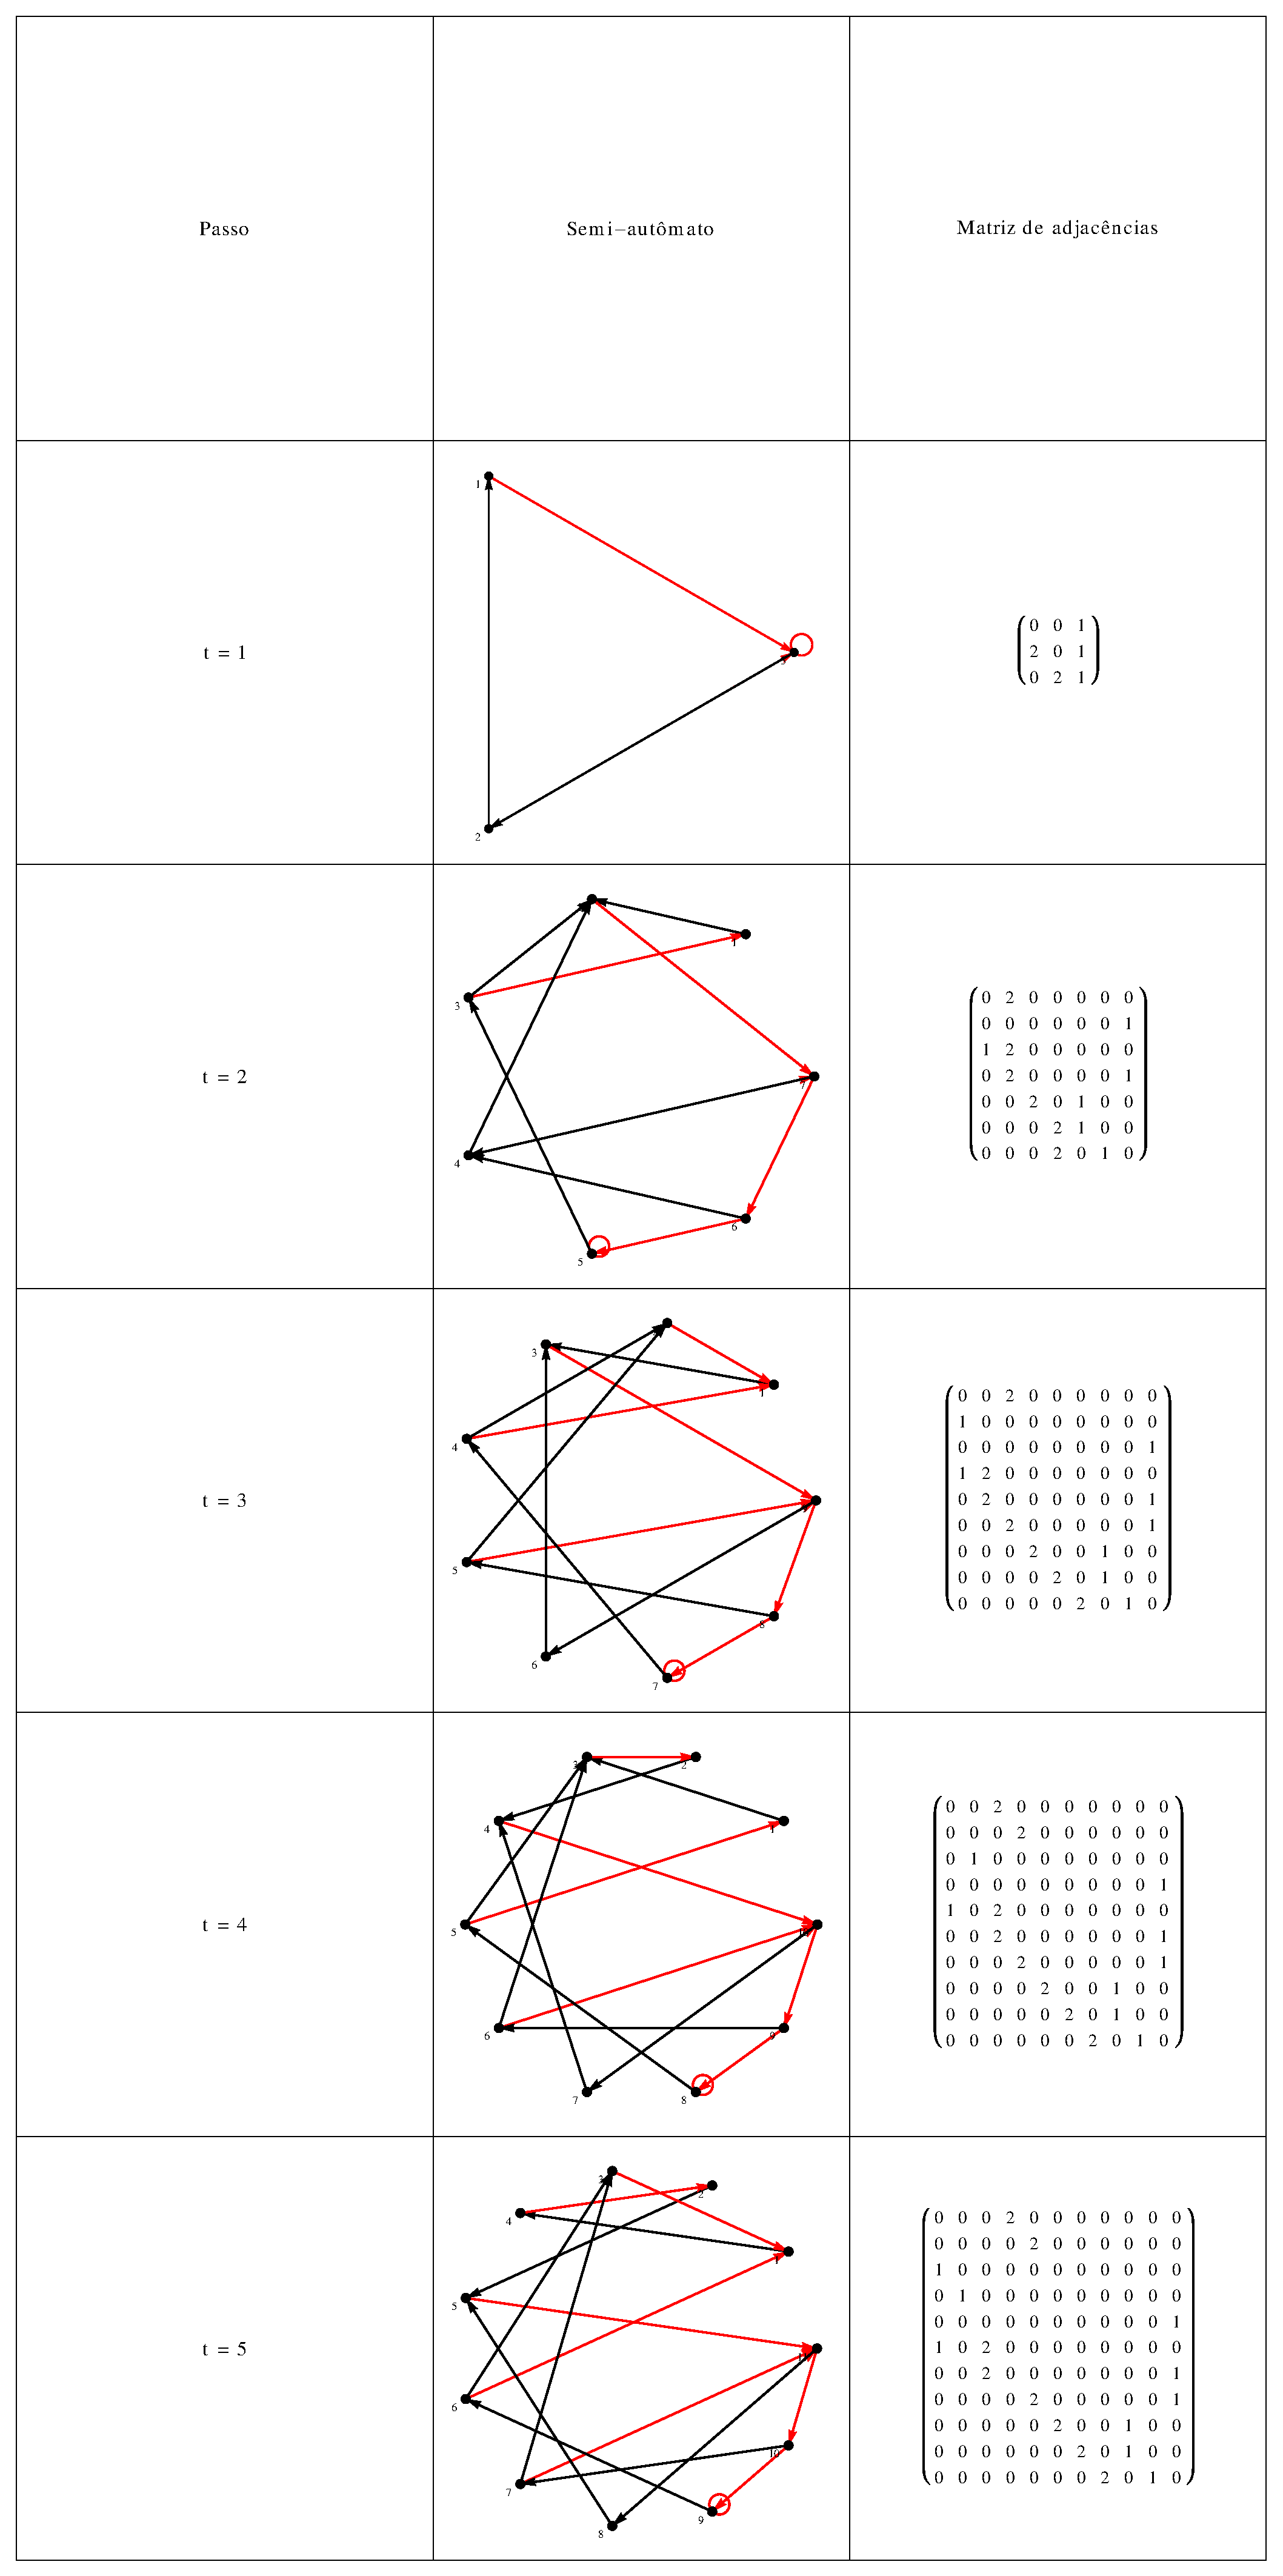
\includegraphics[scale=0.32]{img/mat/matr70.eps}
\caption{Regra 70.}
\label{tab:mr70}
\end{center}
\end{table}

\begin{table}[H]
\begin{center}
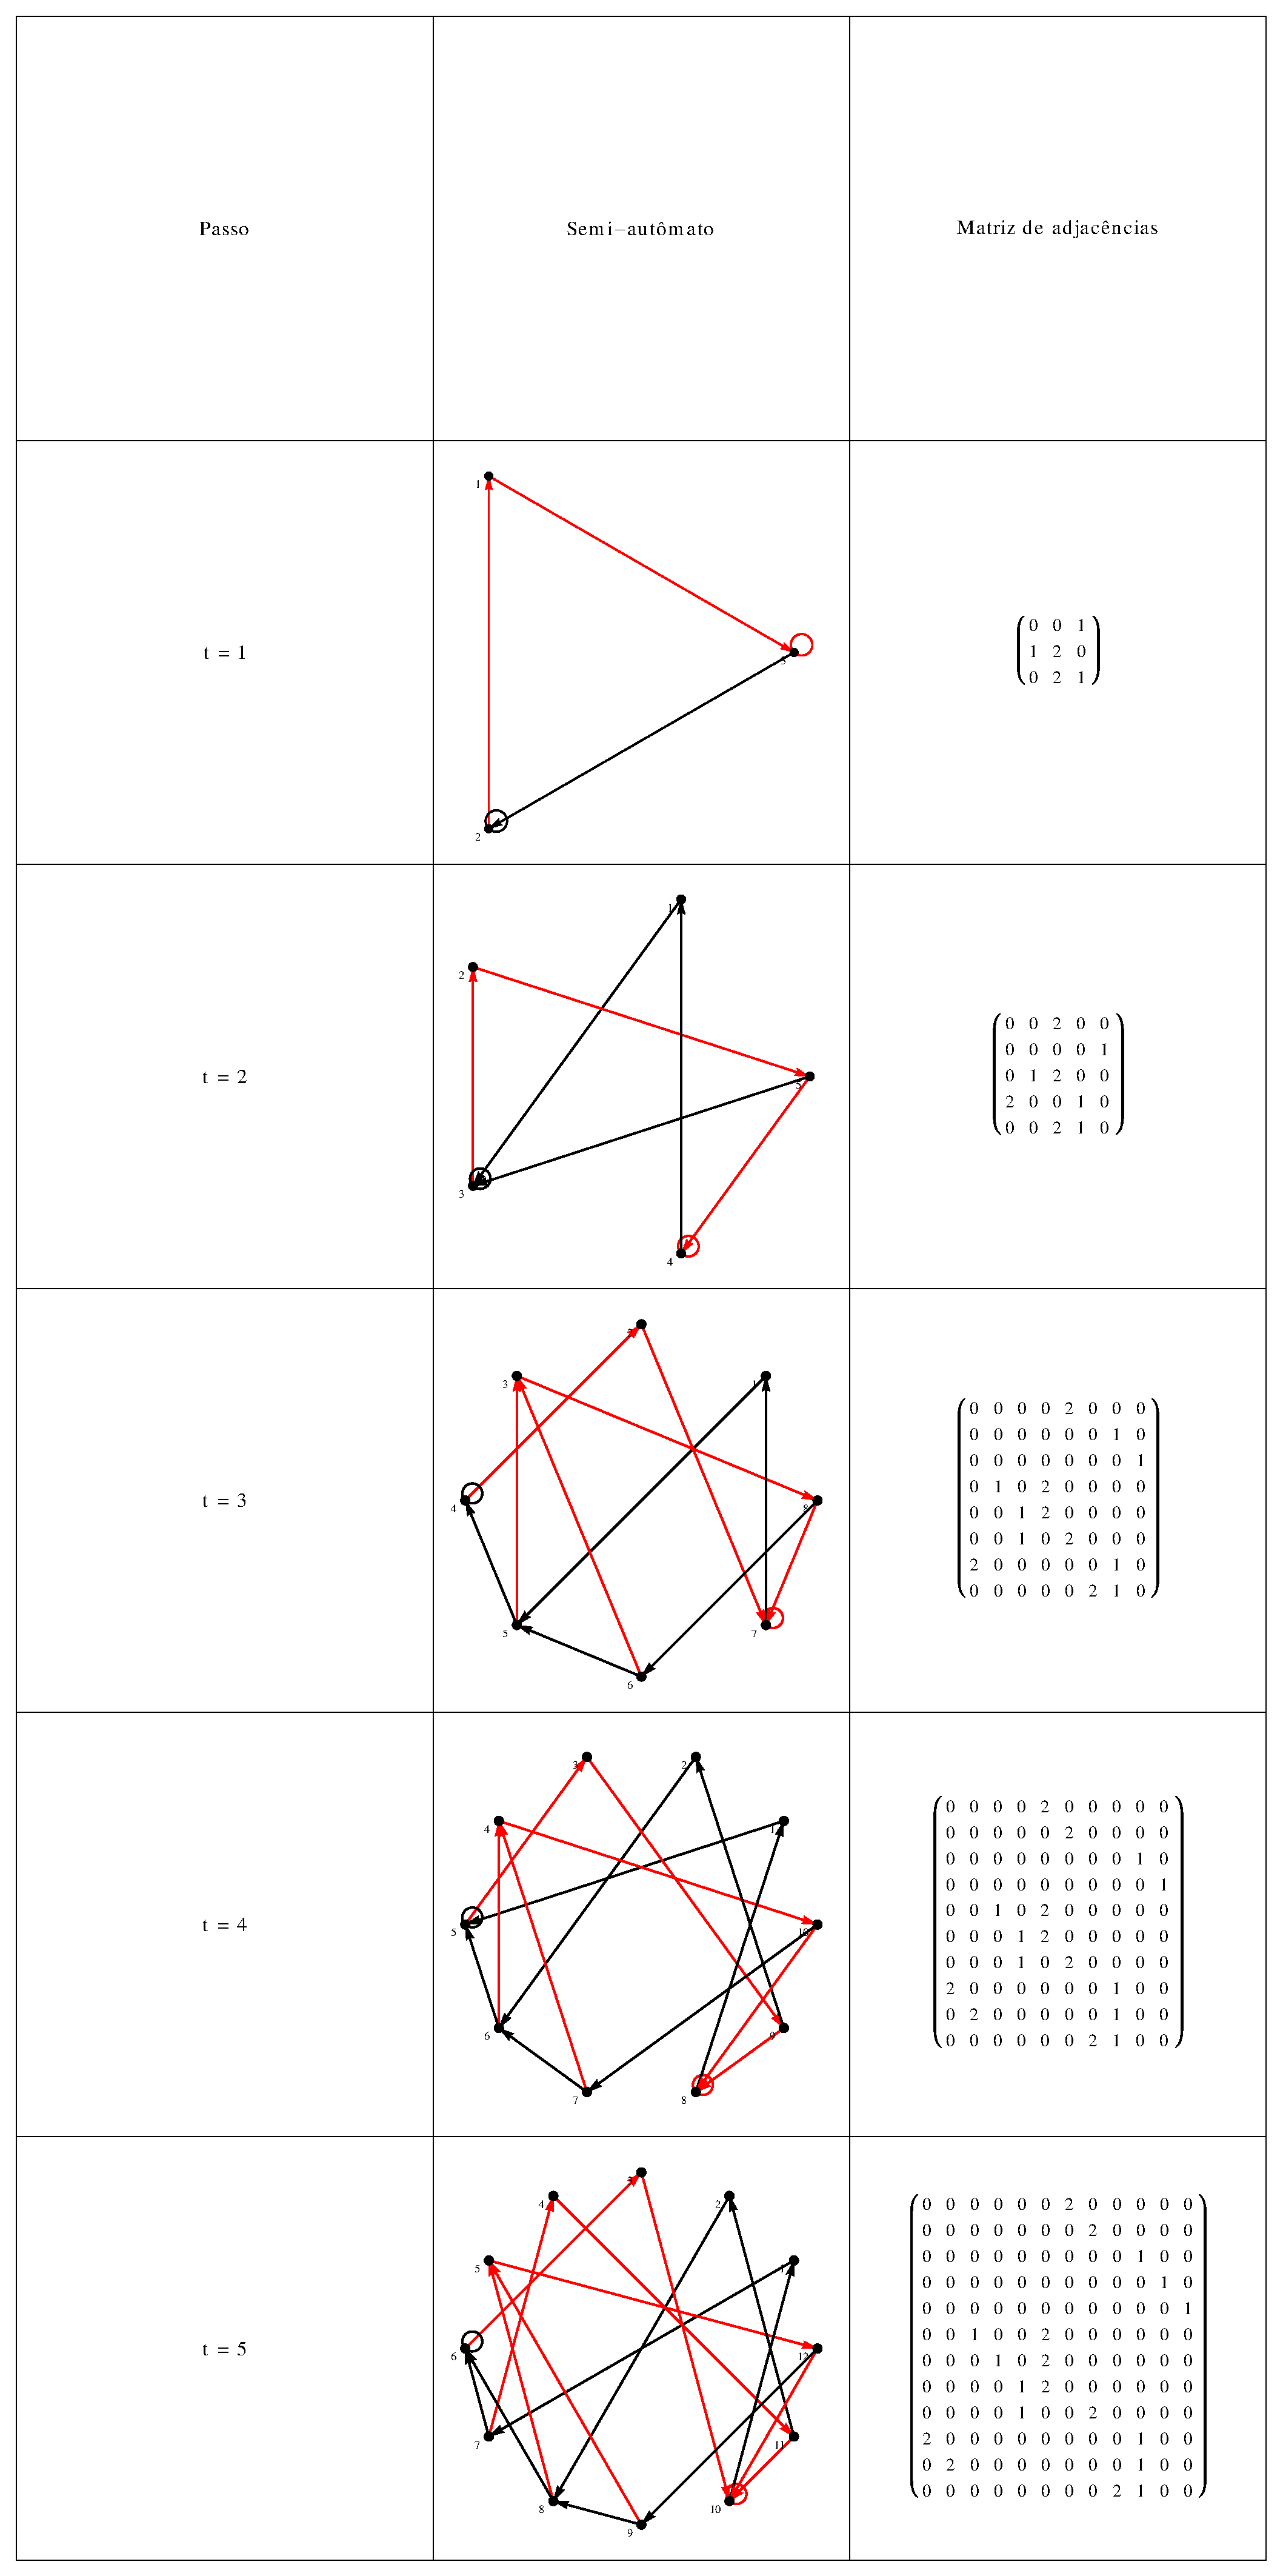
\includegraphics[scale=0.32]{img/mat/matr81.eps}
\caption{Regra 81.}
\label{tab:mr81}
\end{center}
\end{table}

\begin{table}[H]
\begin{center}
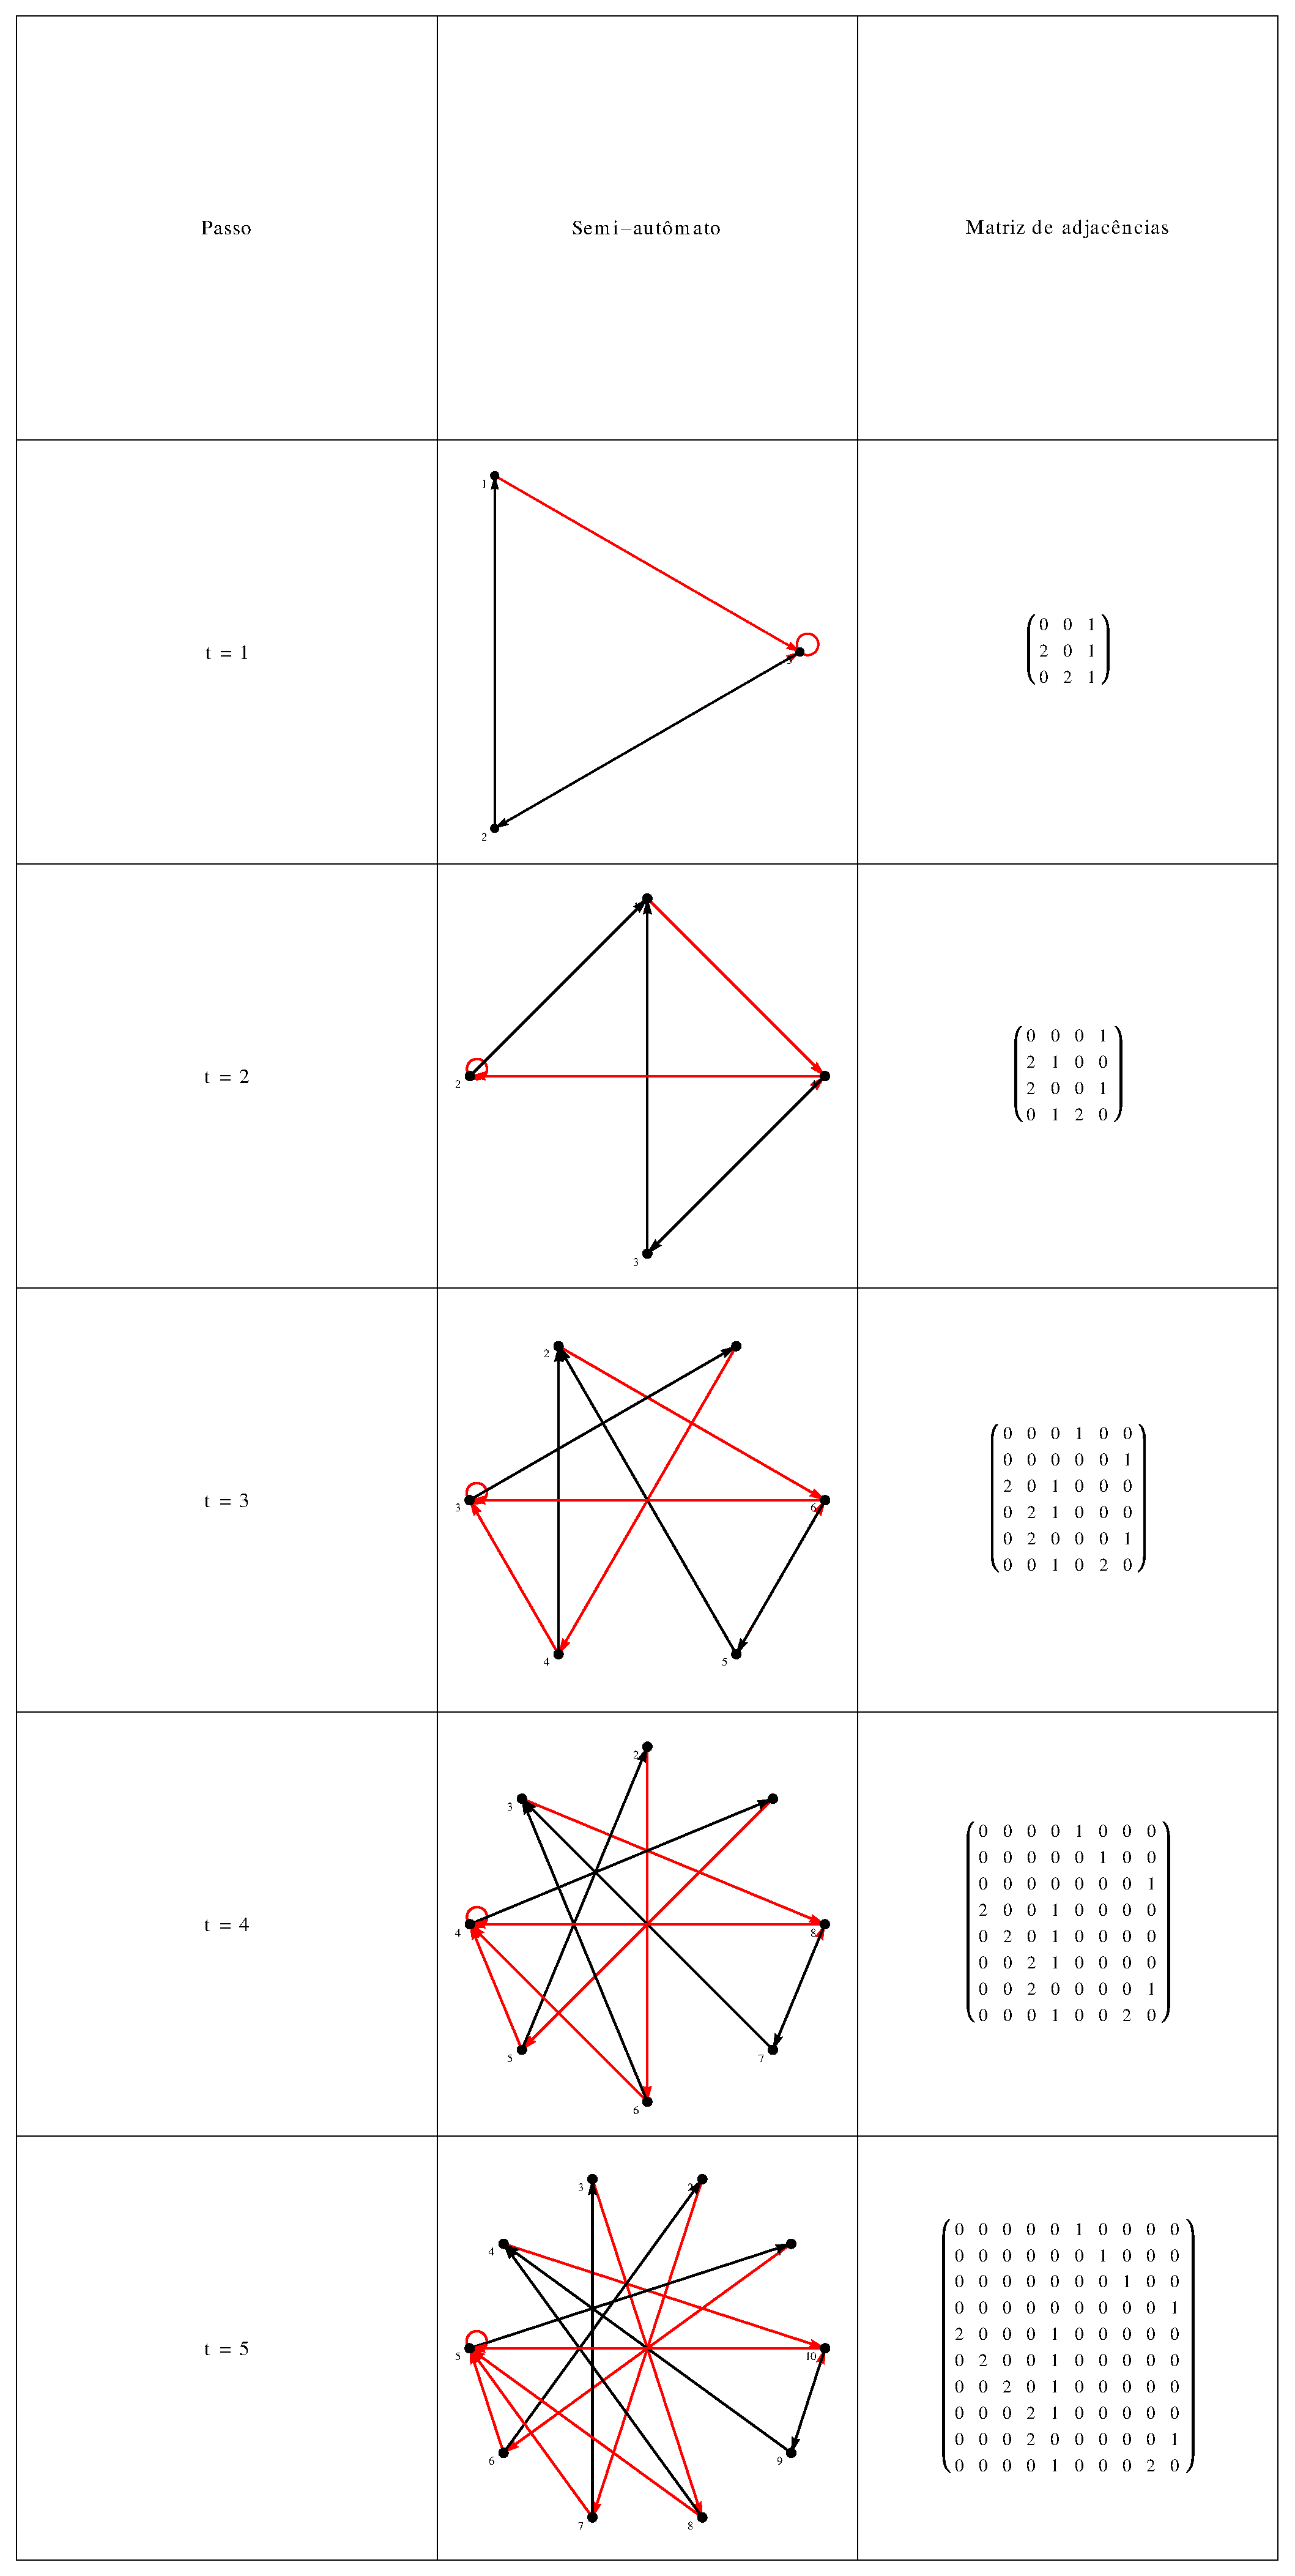
\includegraphics[scale=0.32]{img/mat/matr98.eps}
\caption{Regra 98.}
\label{tab:mr98}
\end{center}
\end{table}

\begin{table}[H]
\begin{center}
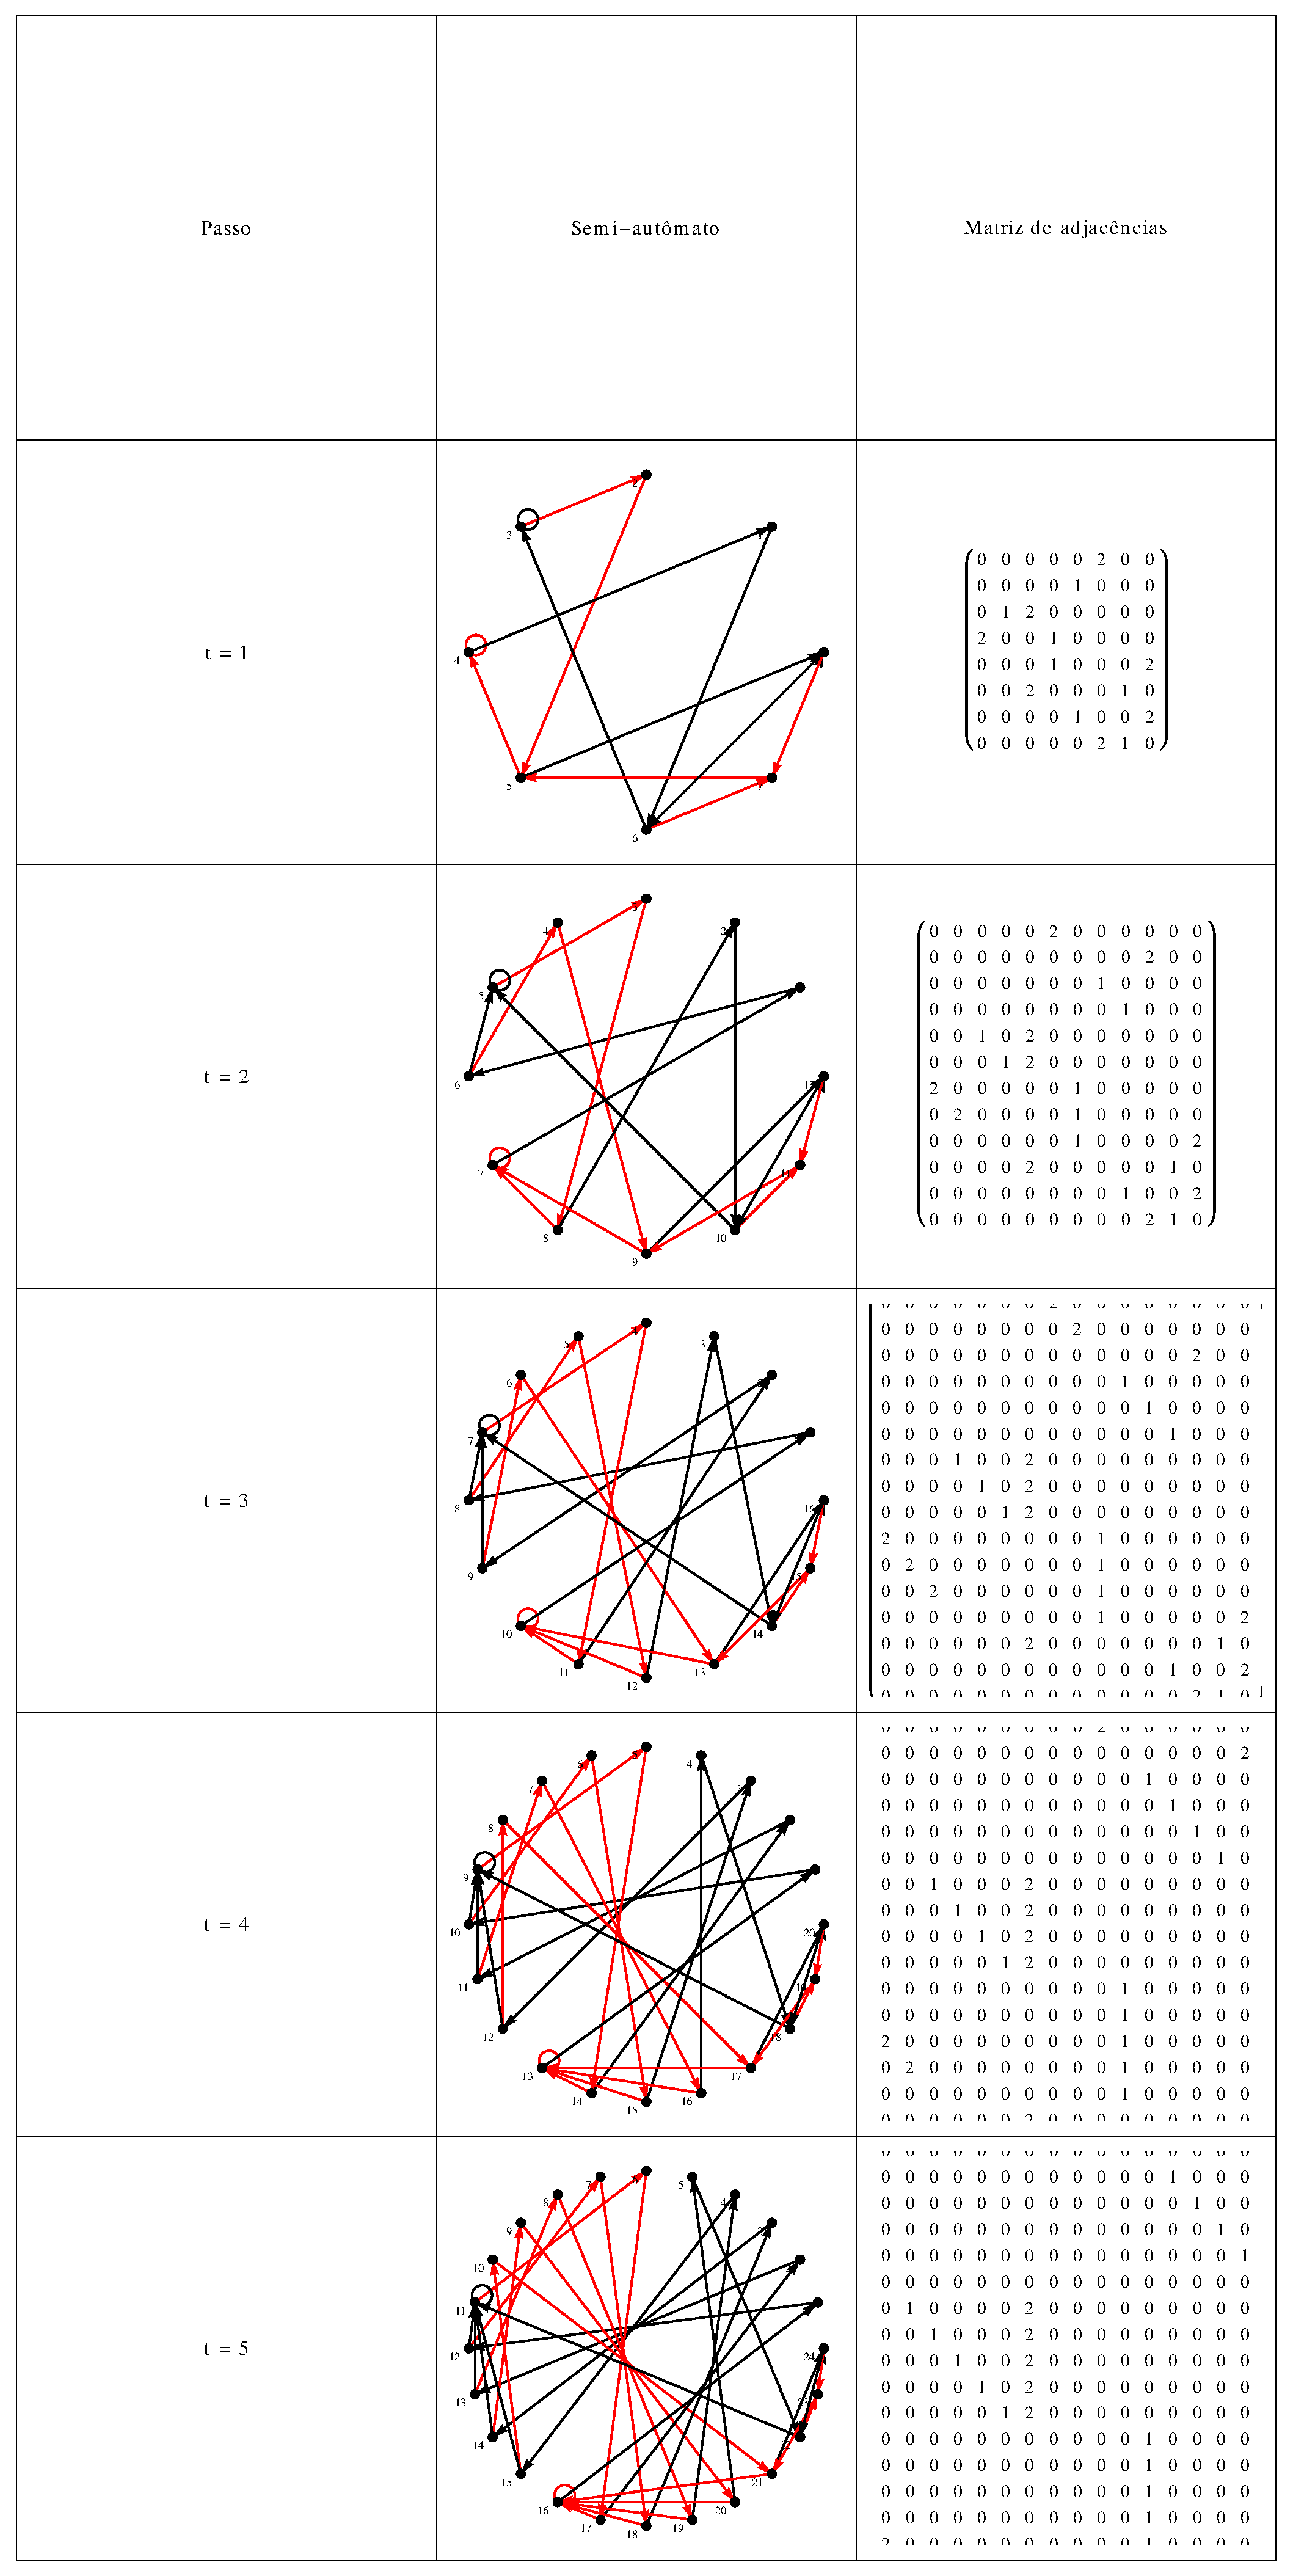
\includegraphics[scale=0.32]{img/mat/matr113.eps}
\caption{Regra 113.}
\label{tab:mr113}
\end{center}
\end{table}

\begin{table}[H]
\begin{center}
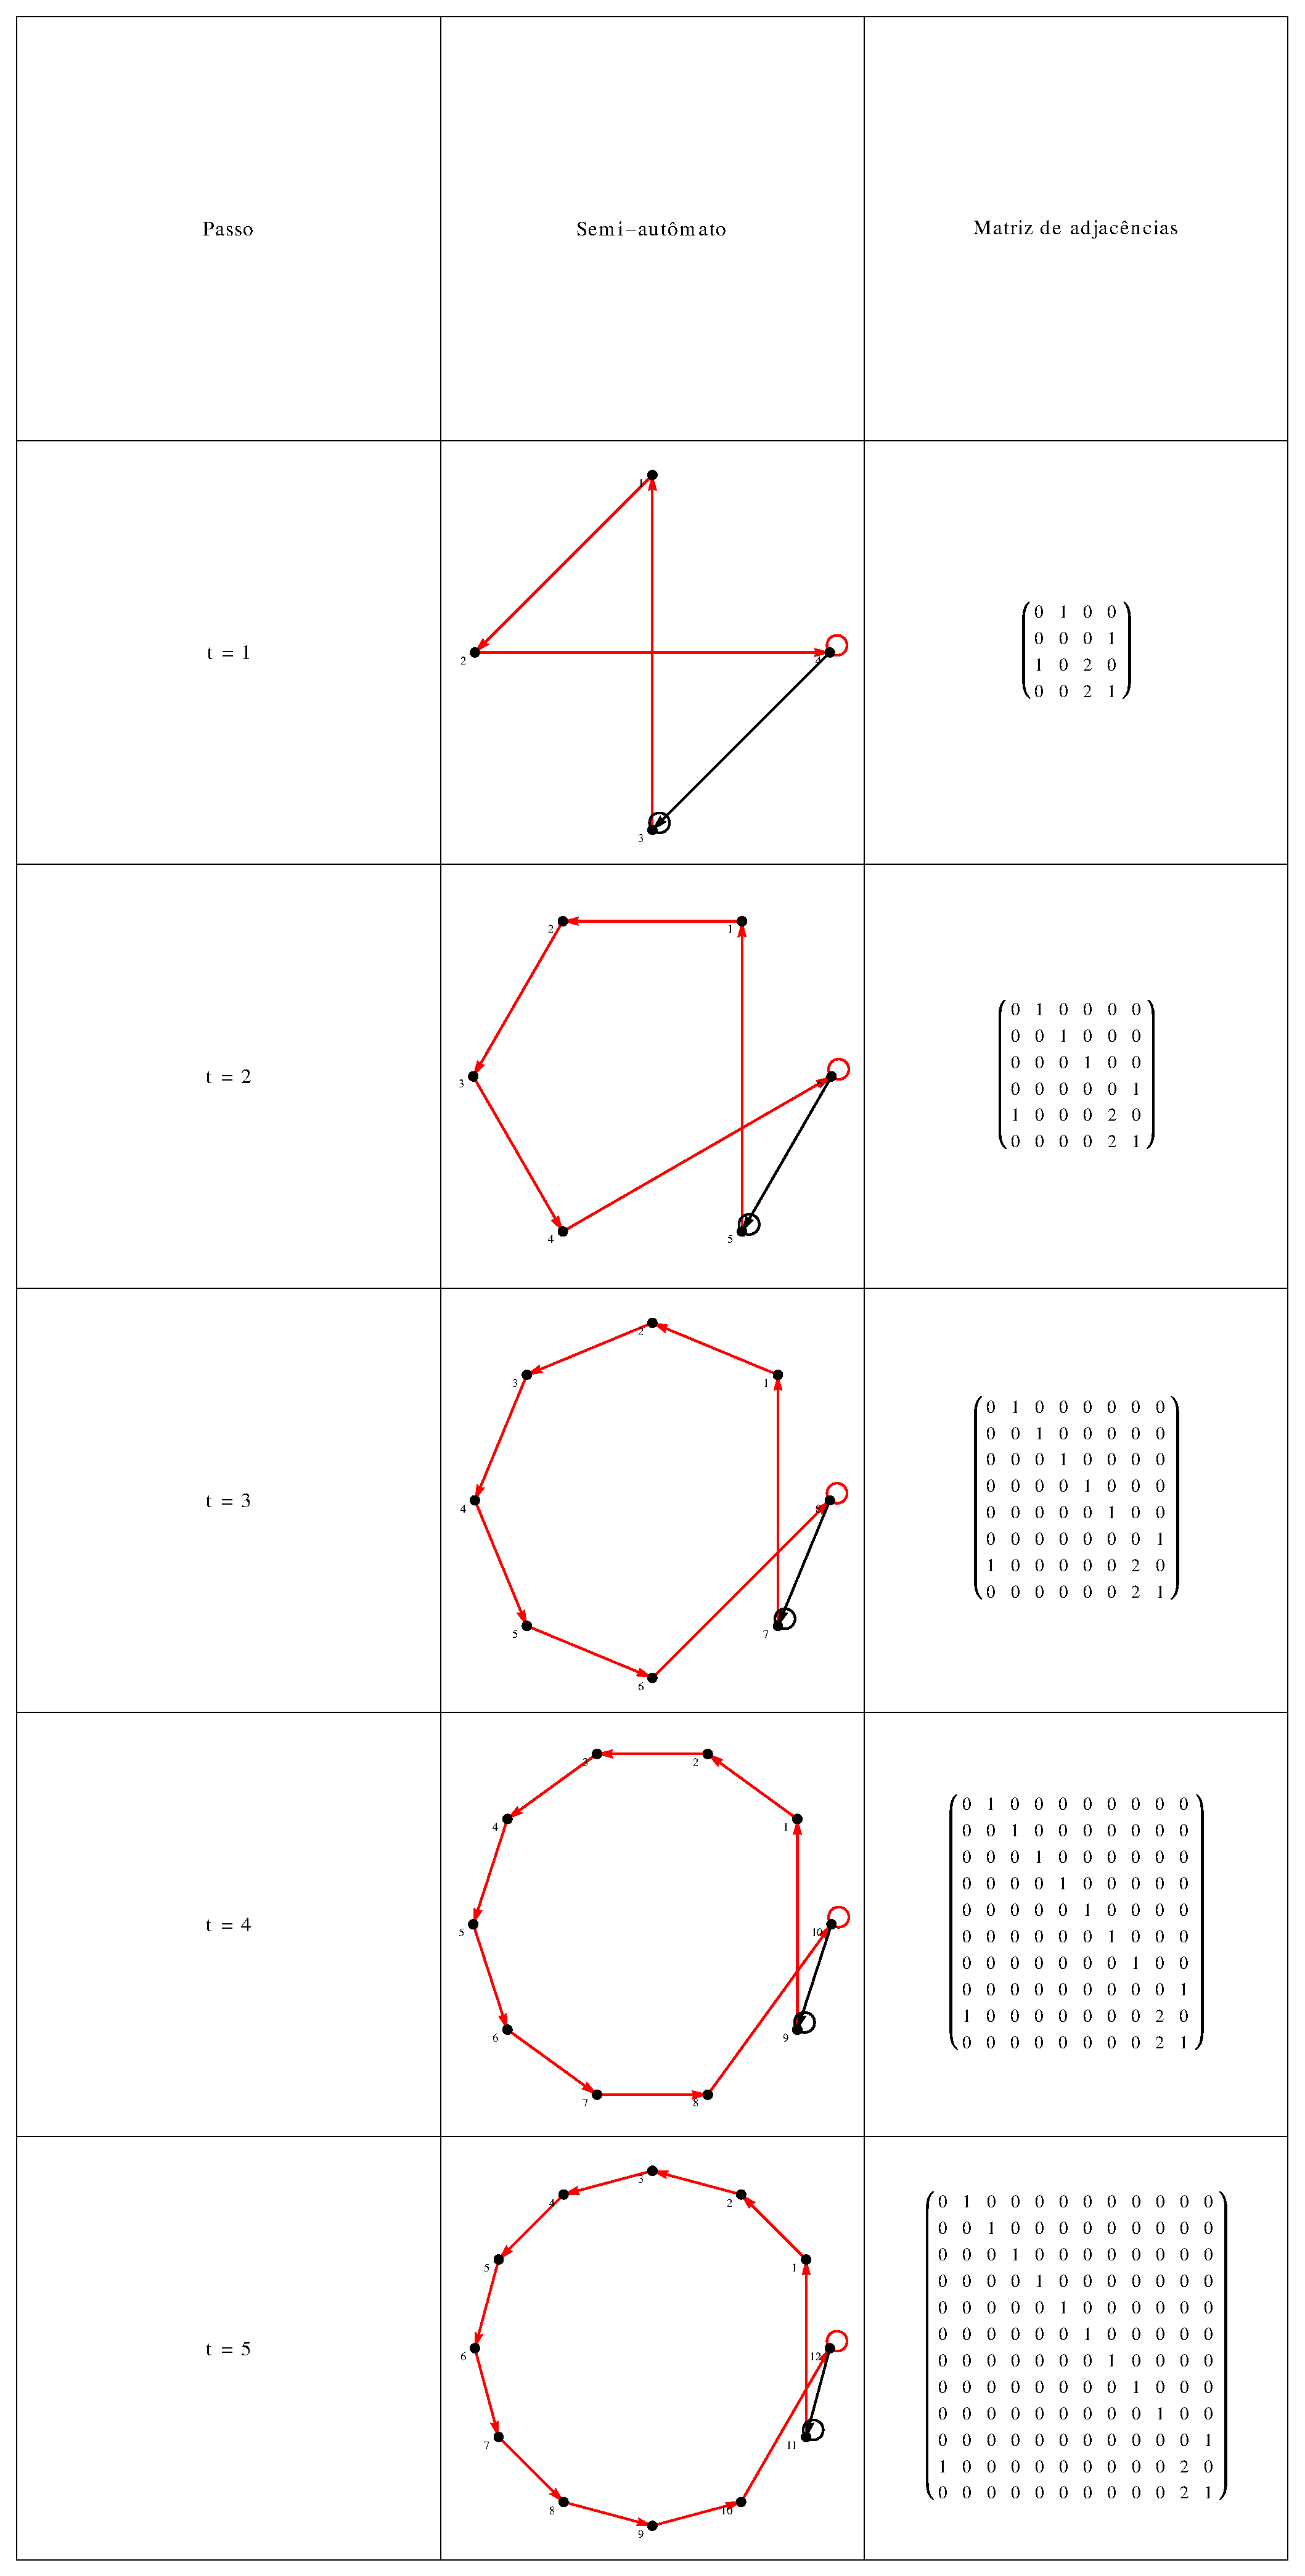
\includegraphics[scale=0.32]{img/mat/matr128.eps}
\caption{Regra 128.}
\label{tab:mr128}
\end{center}
\end{table}

\begin{table}[H]
\begin{center}
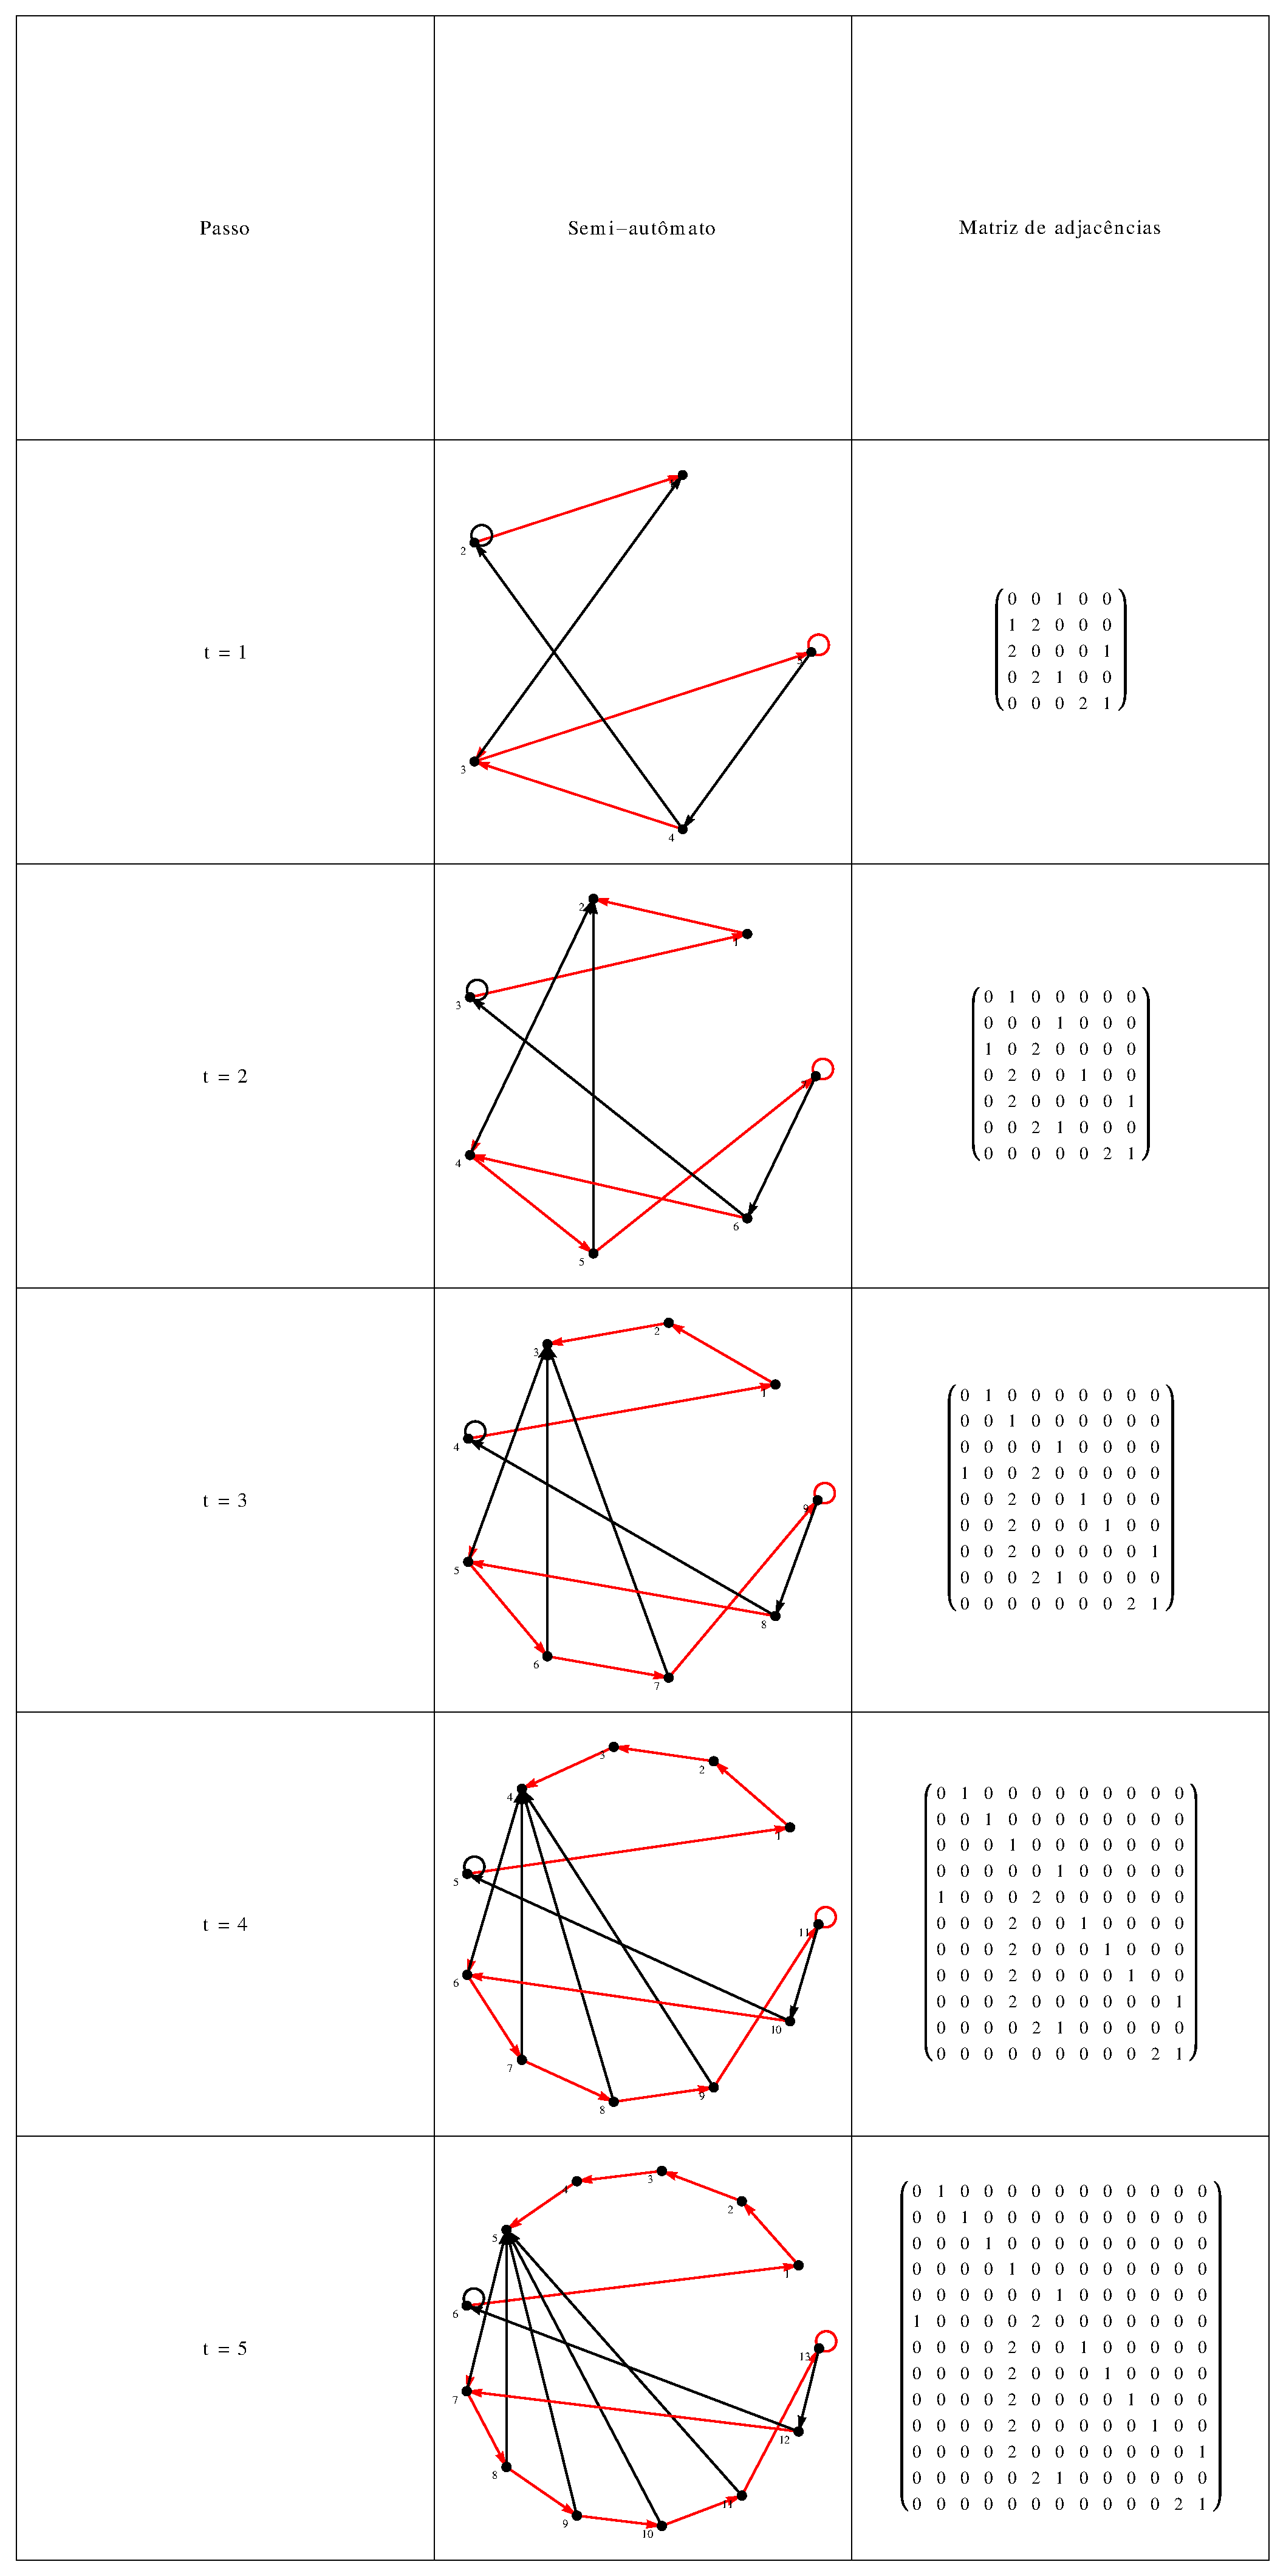
\includegraphics[scale=0.32]{img/mat/matr132.eps}
\caption{Regra 132.}
\label{tab:mr132}
\end{center}
\end{table}

\begin{table}[H]
\begin{center}
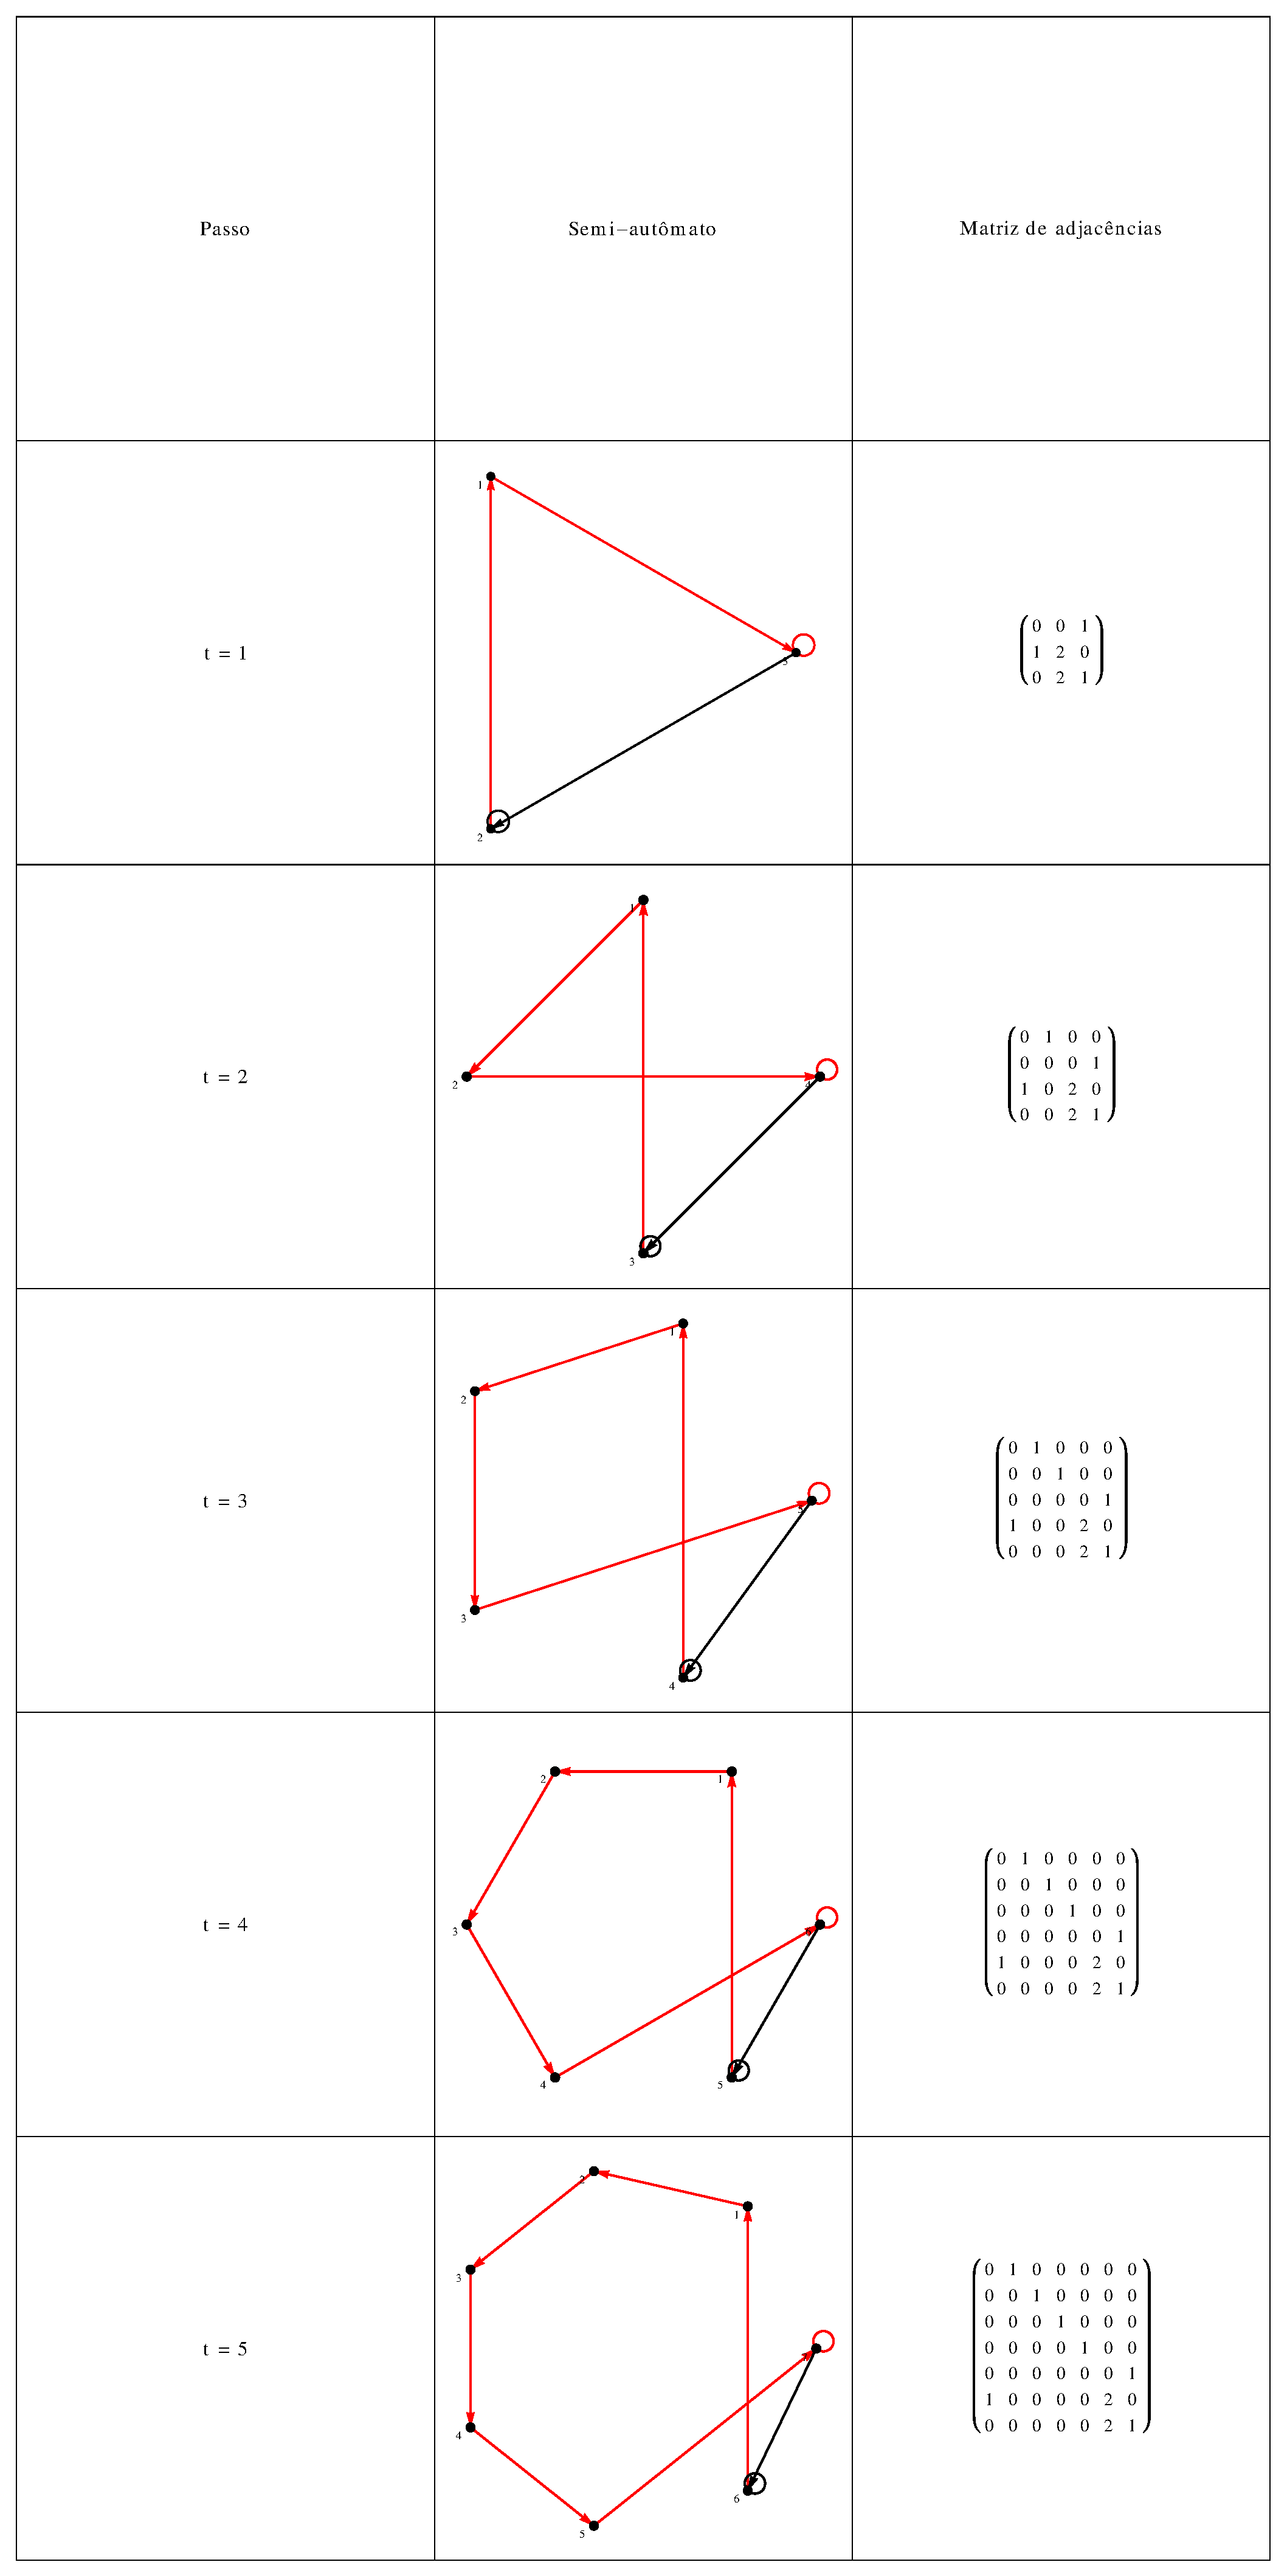
\includegraphics[scale=0.32]{img/mat/matr136.eps}
\caption{Regra 136.}
\label{tab:mr136}
\end{center}
\end{table}

\begin{table}[H]
\begin{center}
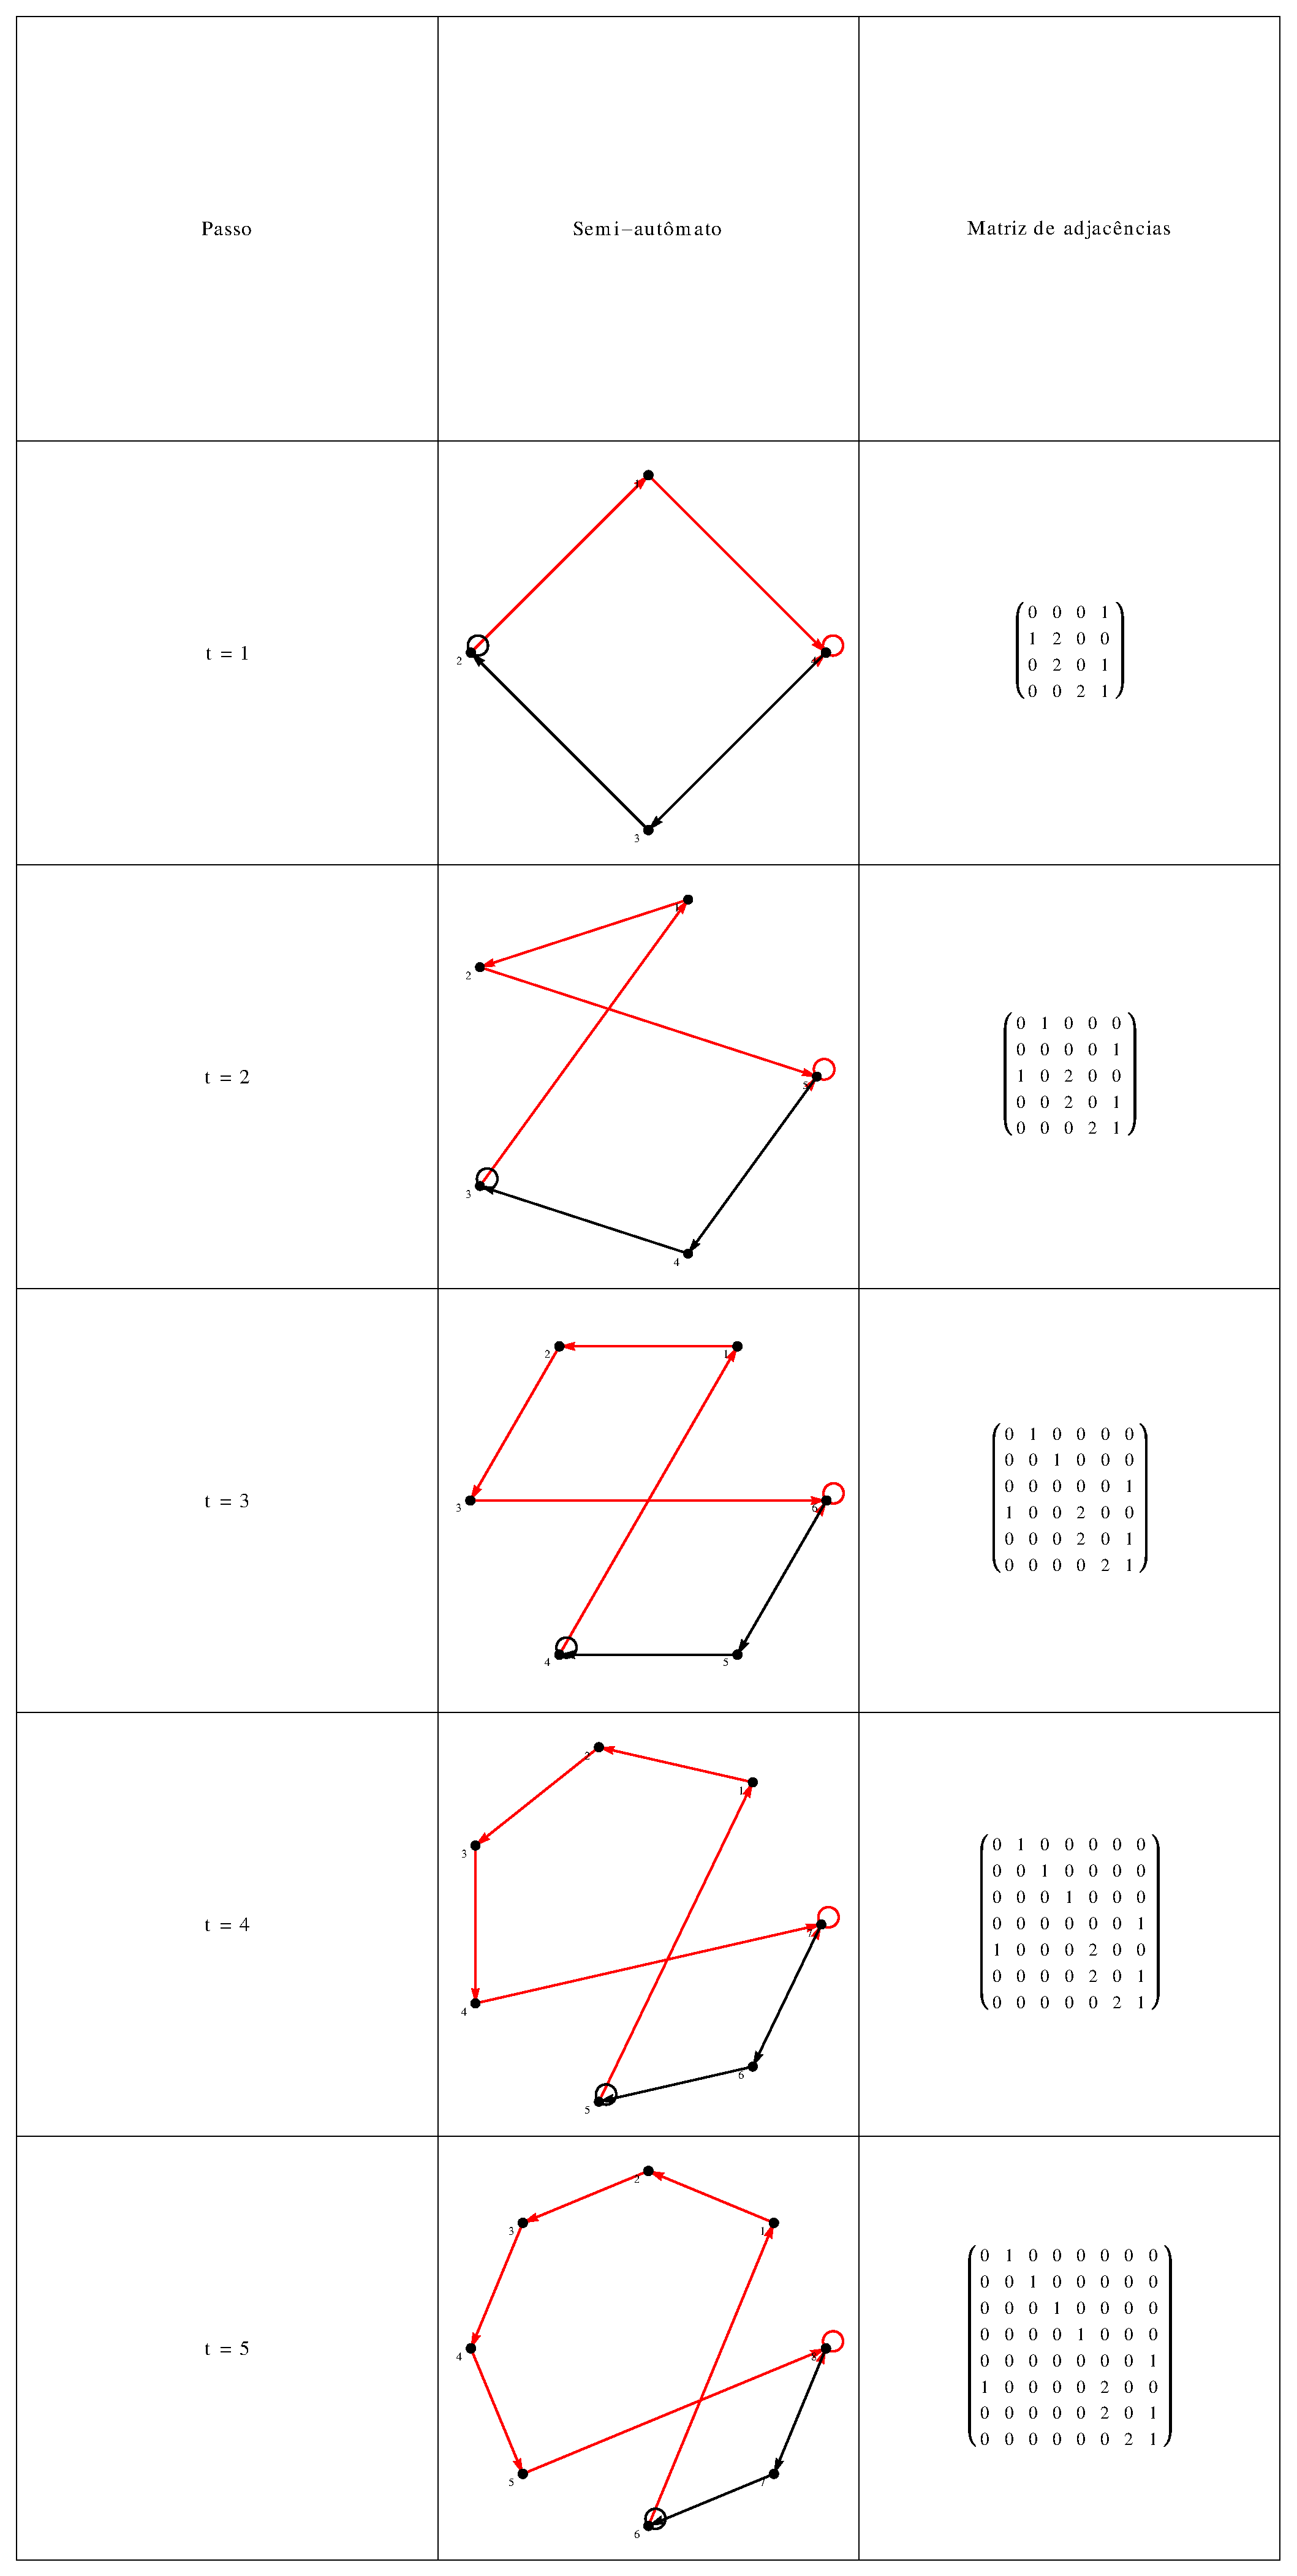
\includegraphics[scale=0.32]{img/mat/matr140.eps}
\caption{Regra 140.}
\label{tab:mr140}
\end{center}
\end{table}

\begin{table}[H]
\begin{center}
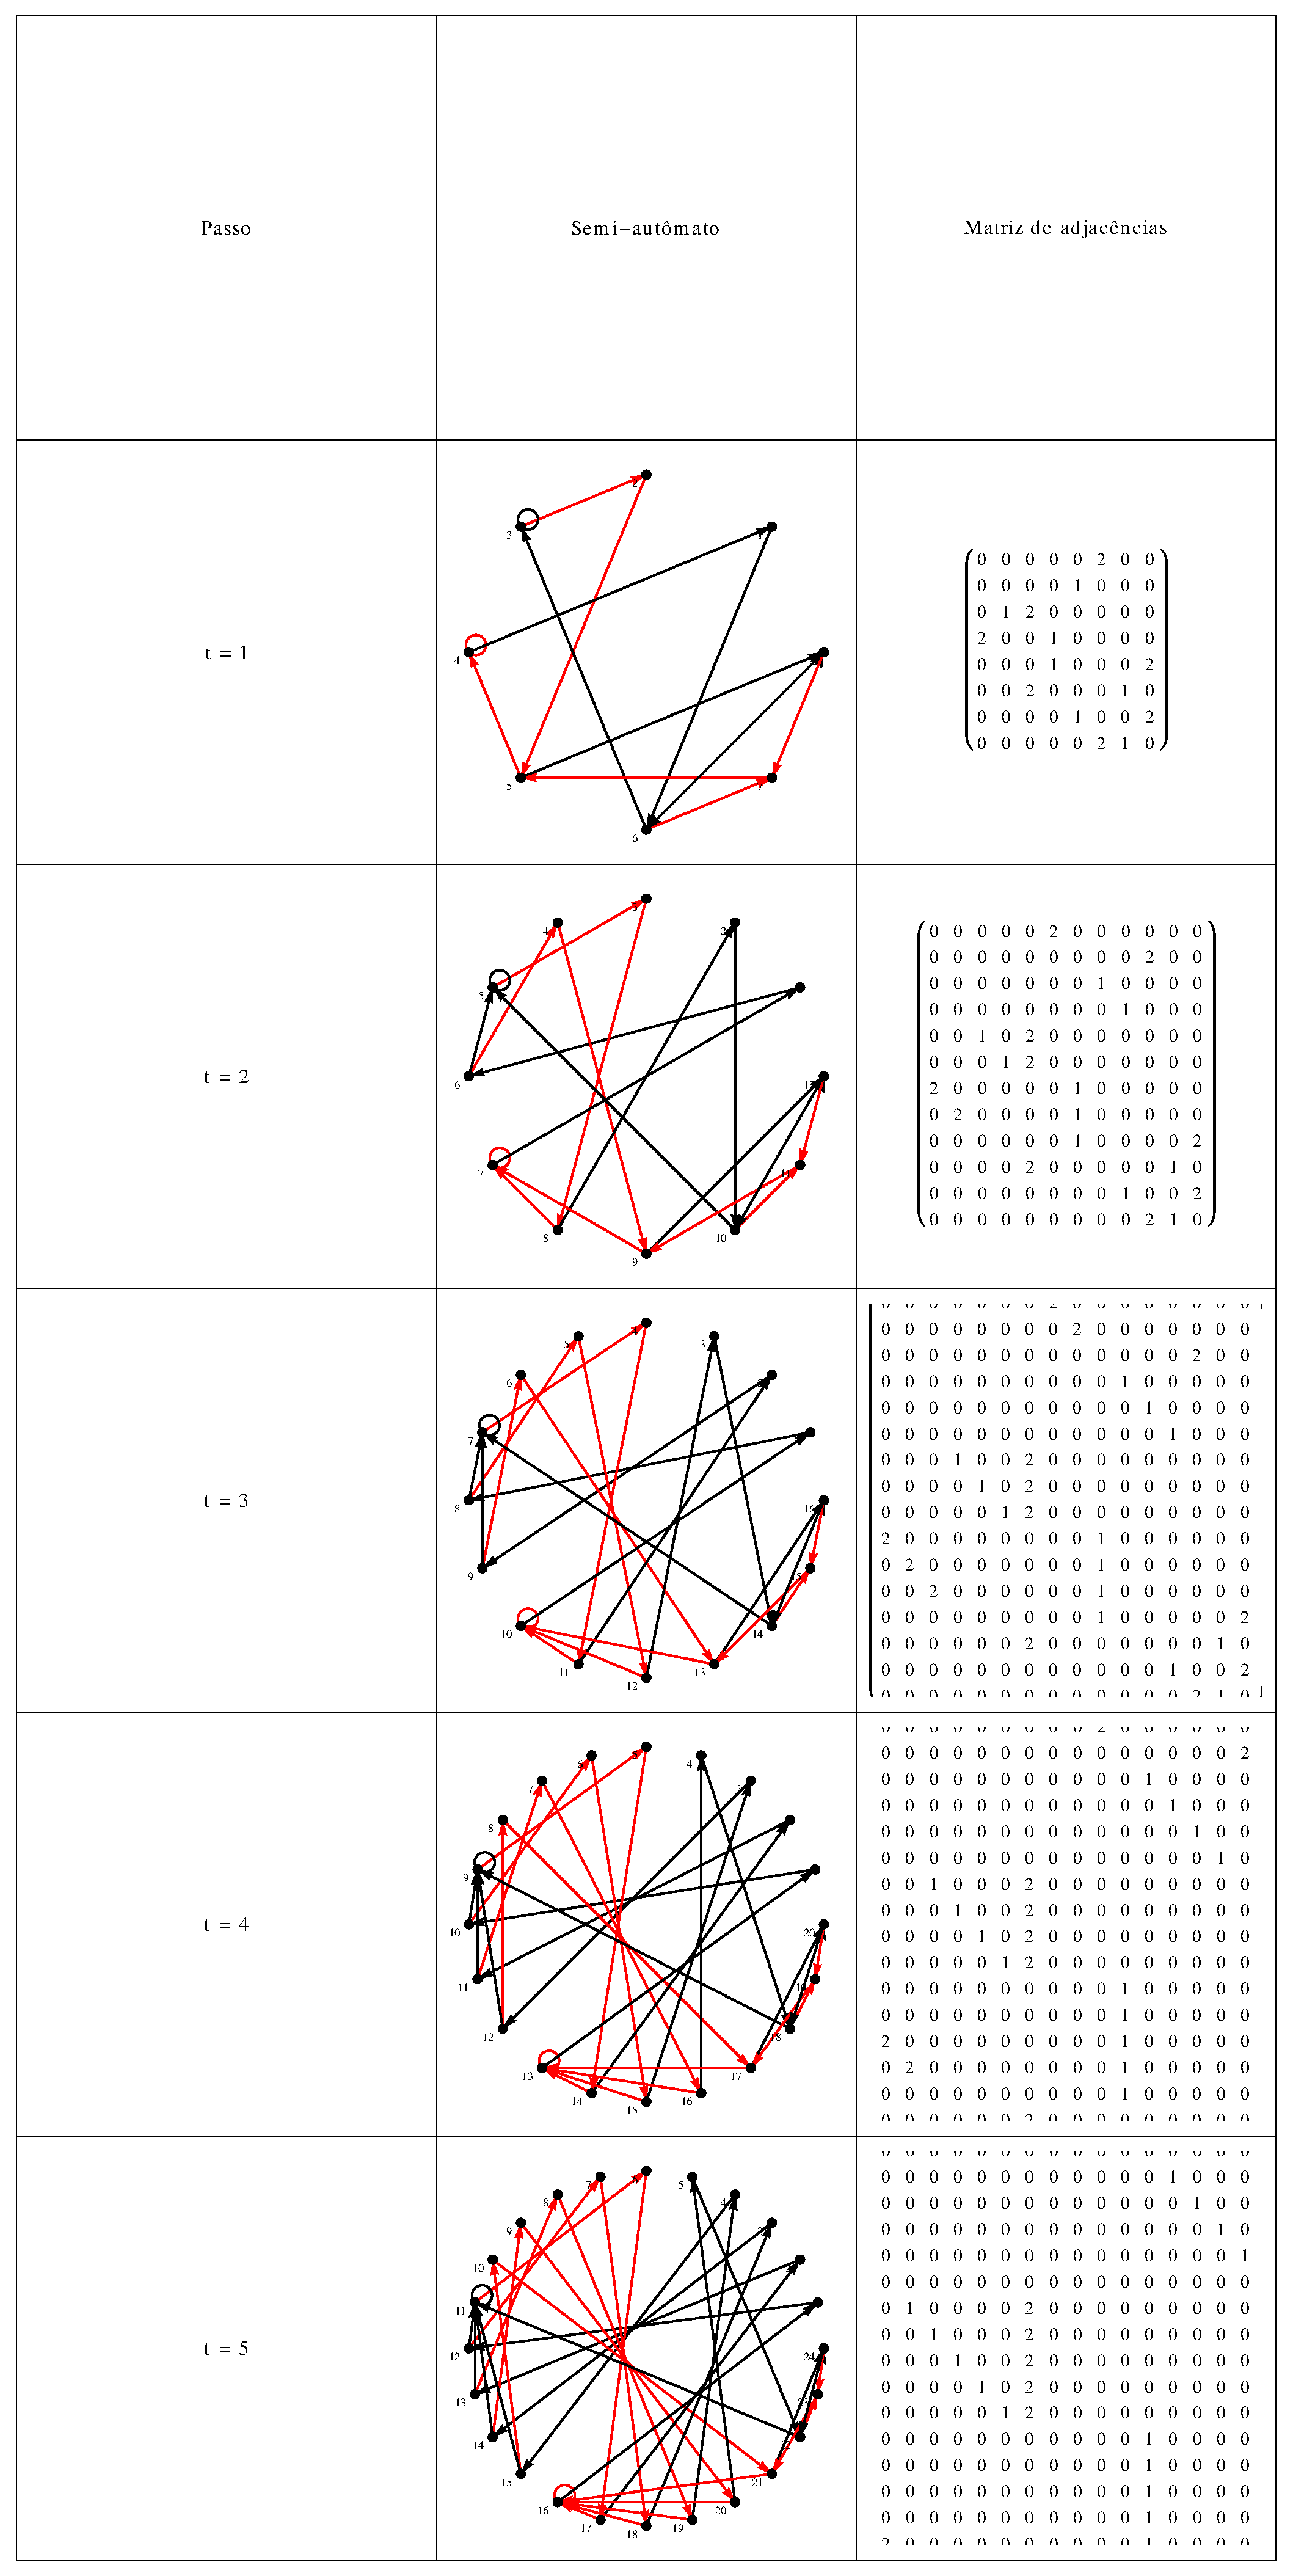
\includegraphics[scale=0.32]{img/mat/matr142.eps}
\caption{Regra 142.}
\label{tab:mr142}
\end{center}
\end{table}

\begin{table}[H]
\begin{center}
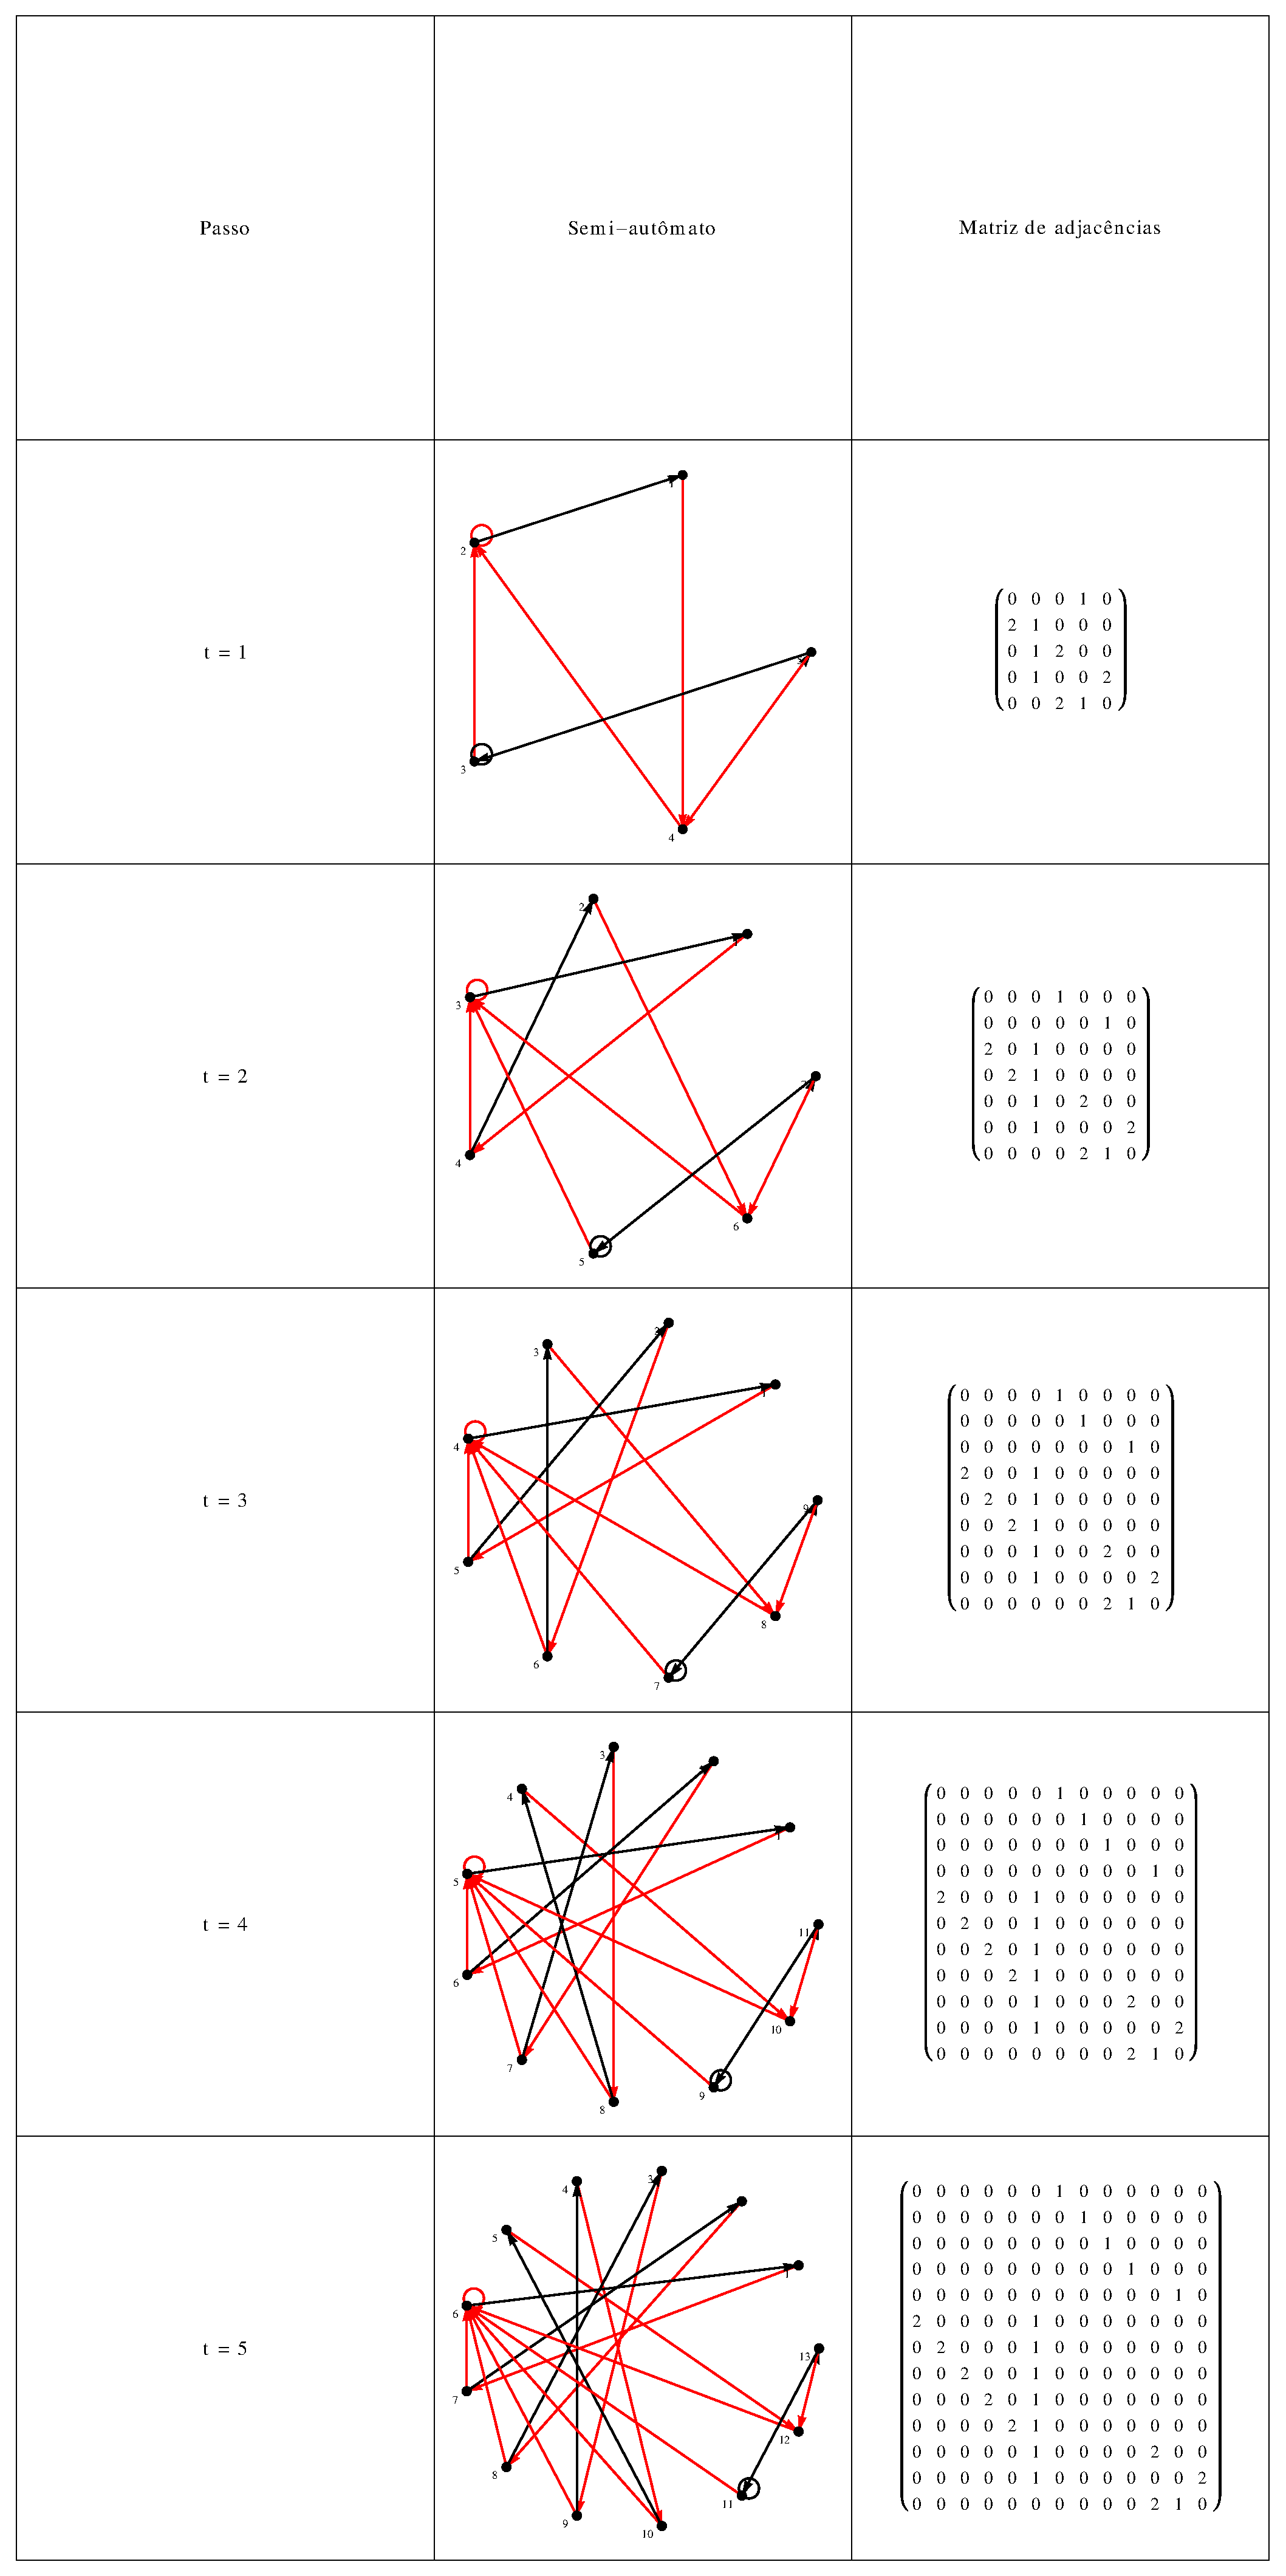
\includegraphics[scale=0.32]{img/mat/matr162.eps}
\caption{Regra 162.}
\label{tab:mr162}
\end{center}
\end{table}

\begin{table}[H]
\begin{center}
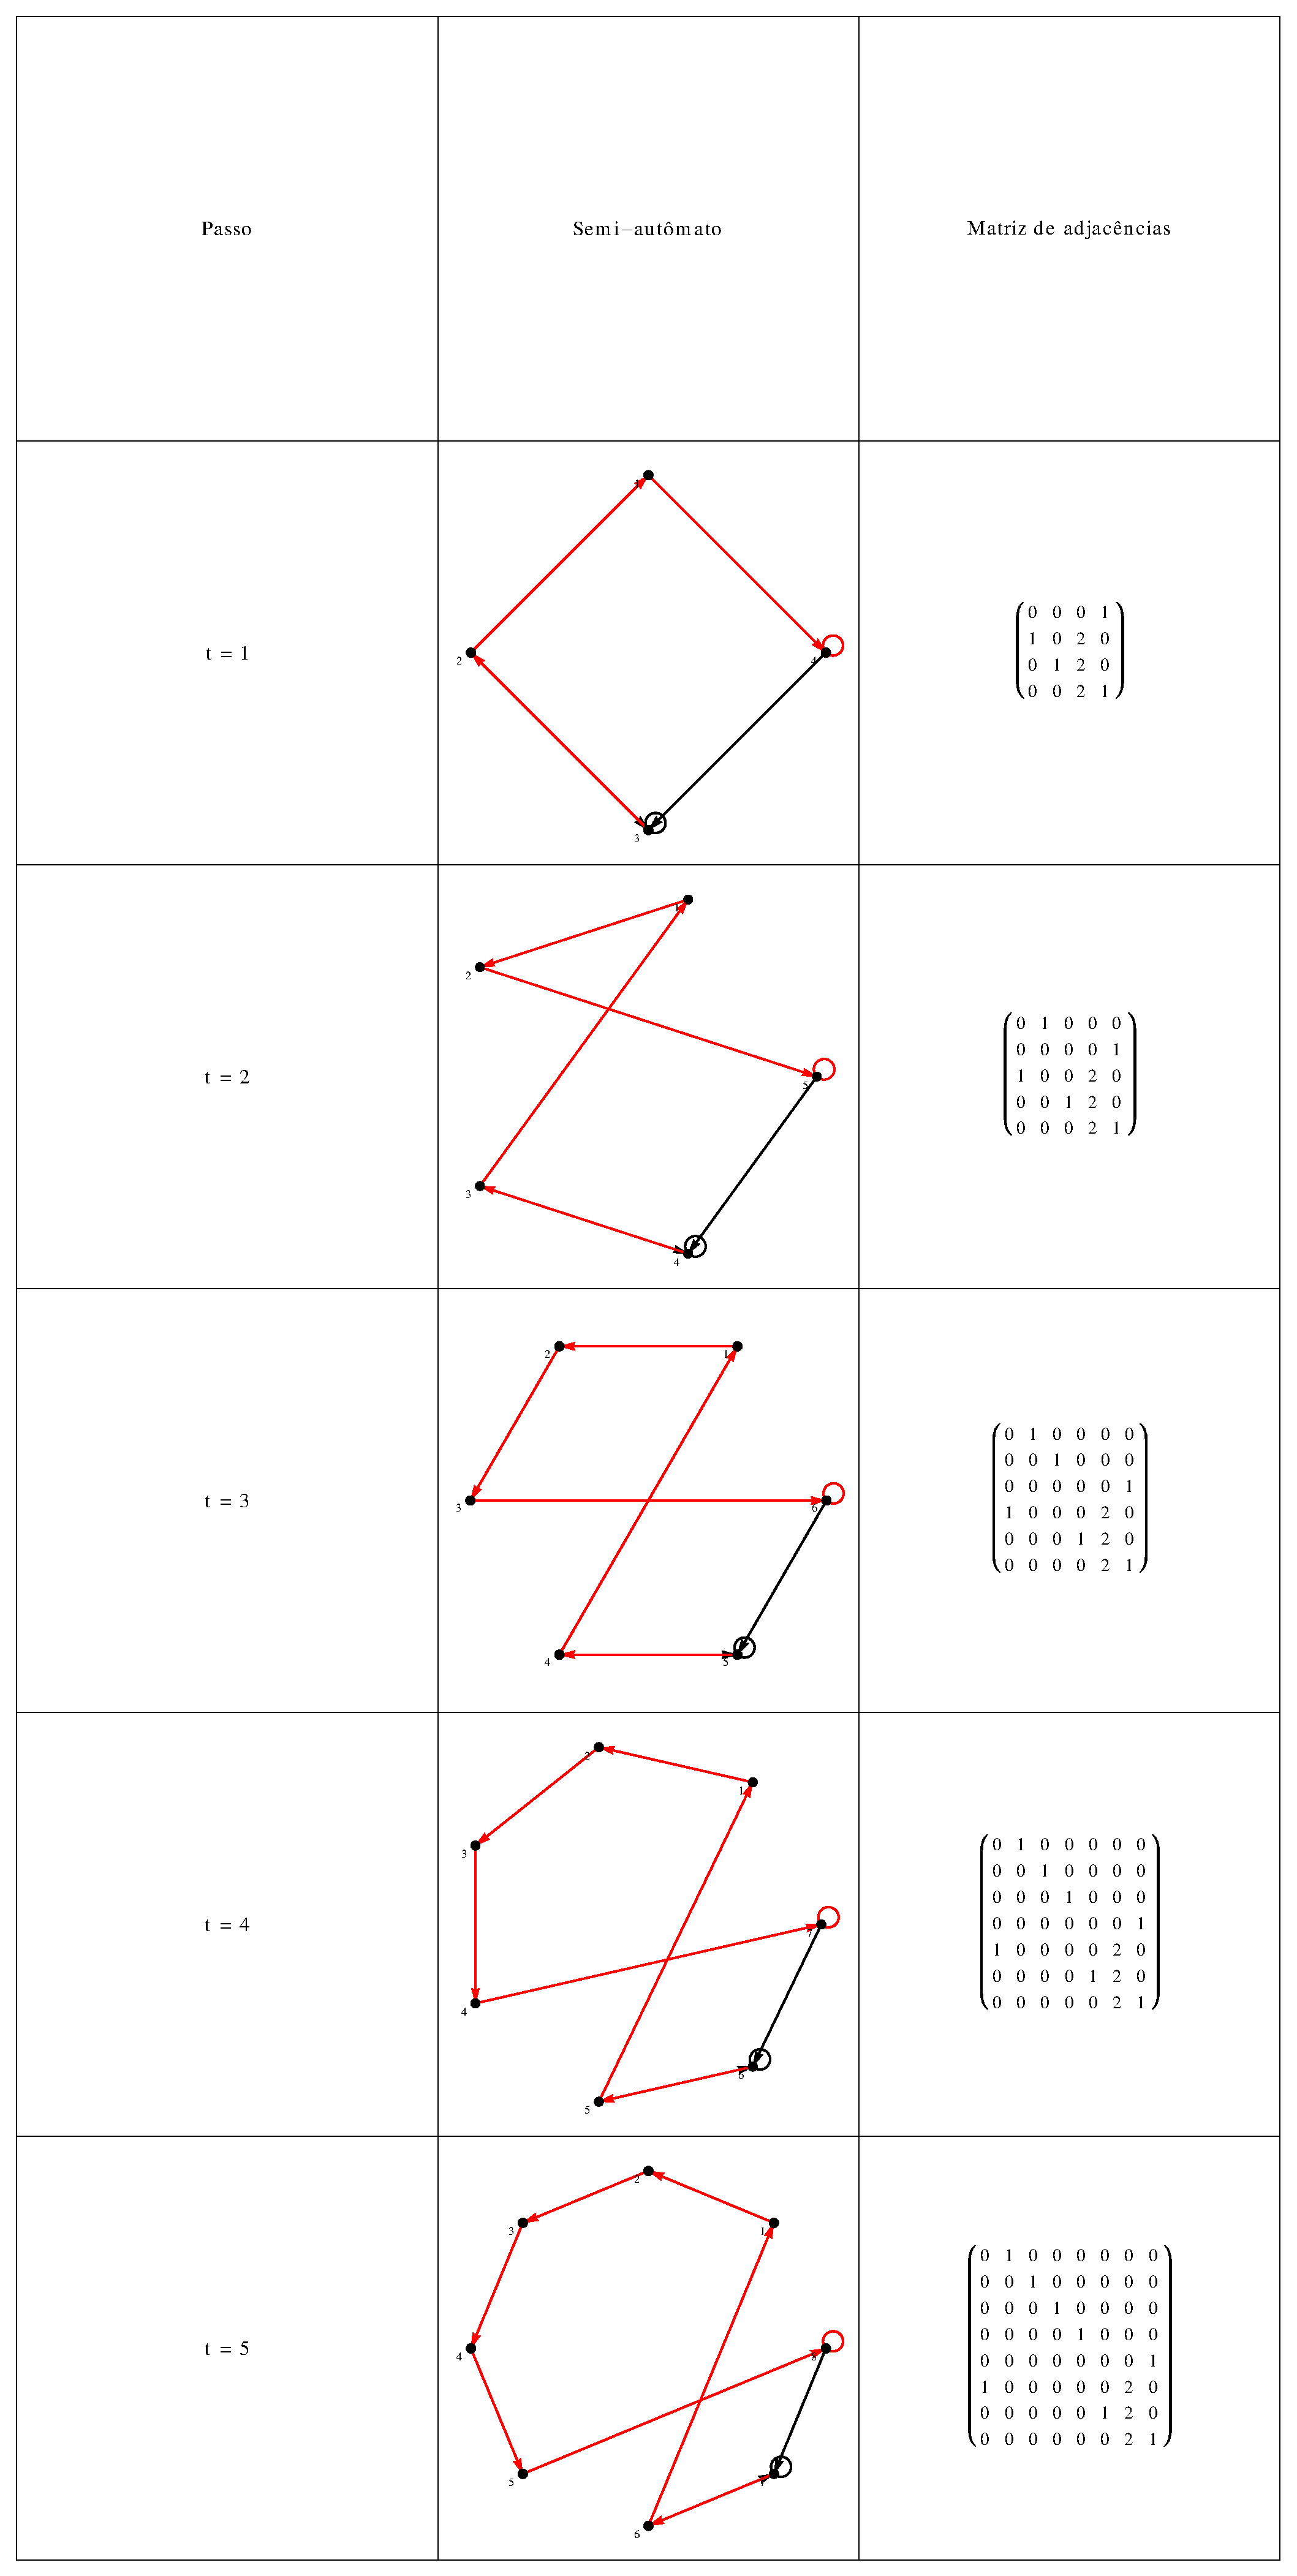
\includegraphics[scale=0.32]{img/mat/matr168.eps}
\caption{Regra 168.}
\label{tab:mr168}
\end{center}
\end{table}

\begin{table}[H]
\begin{center}
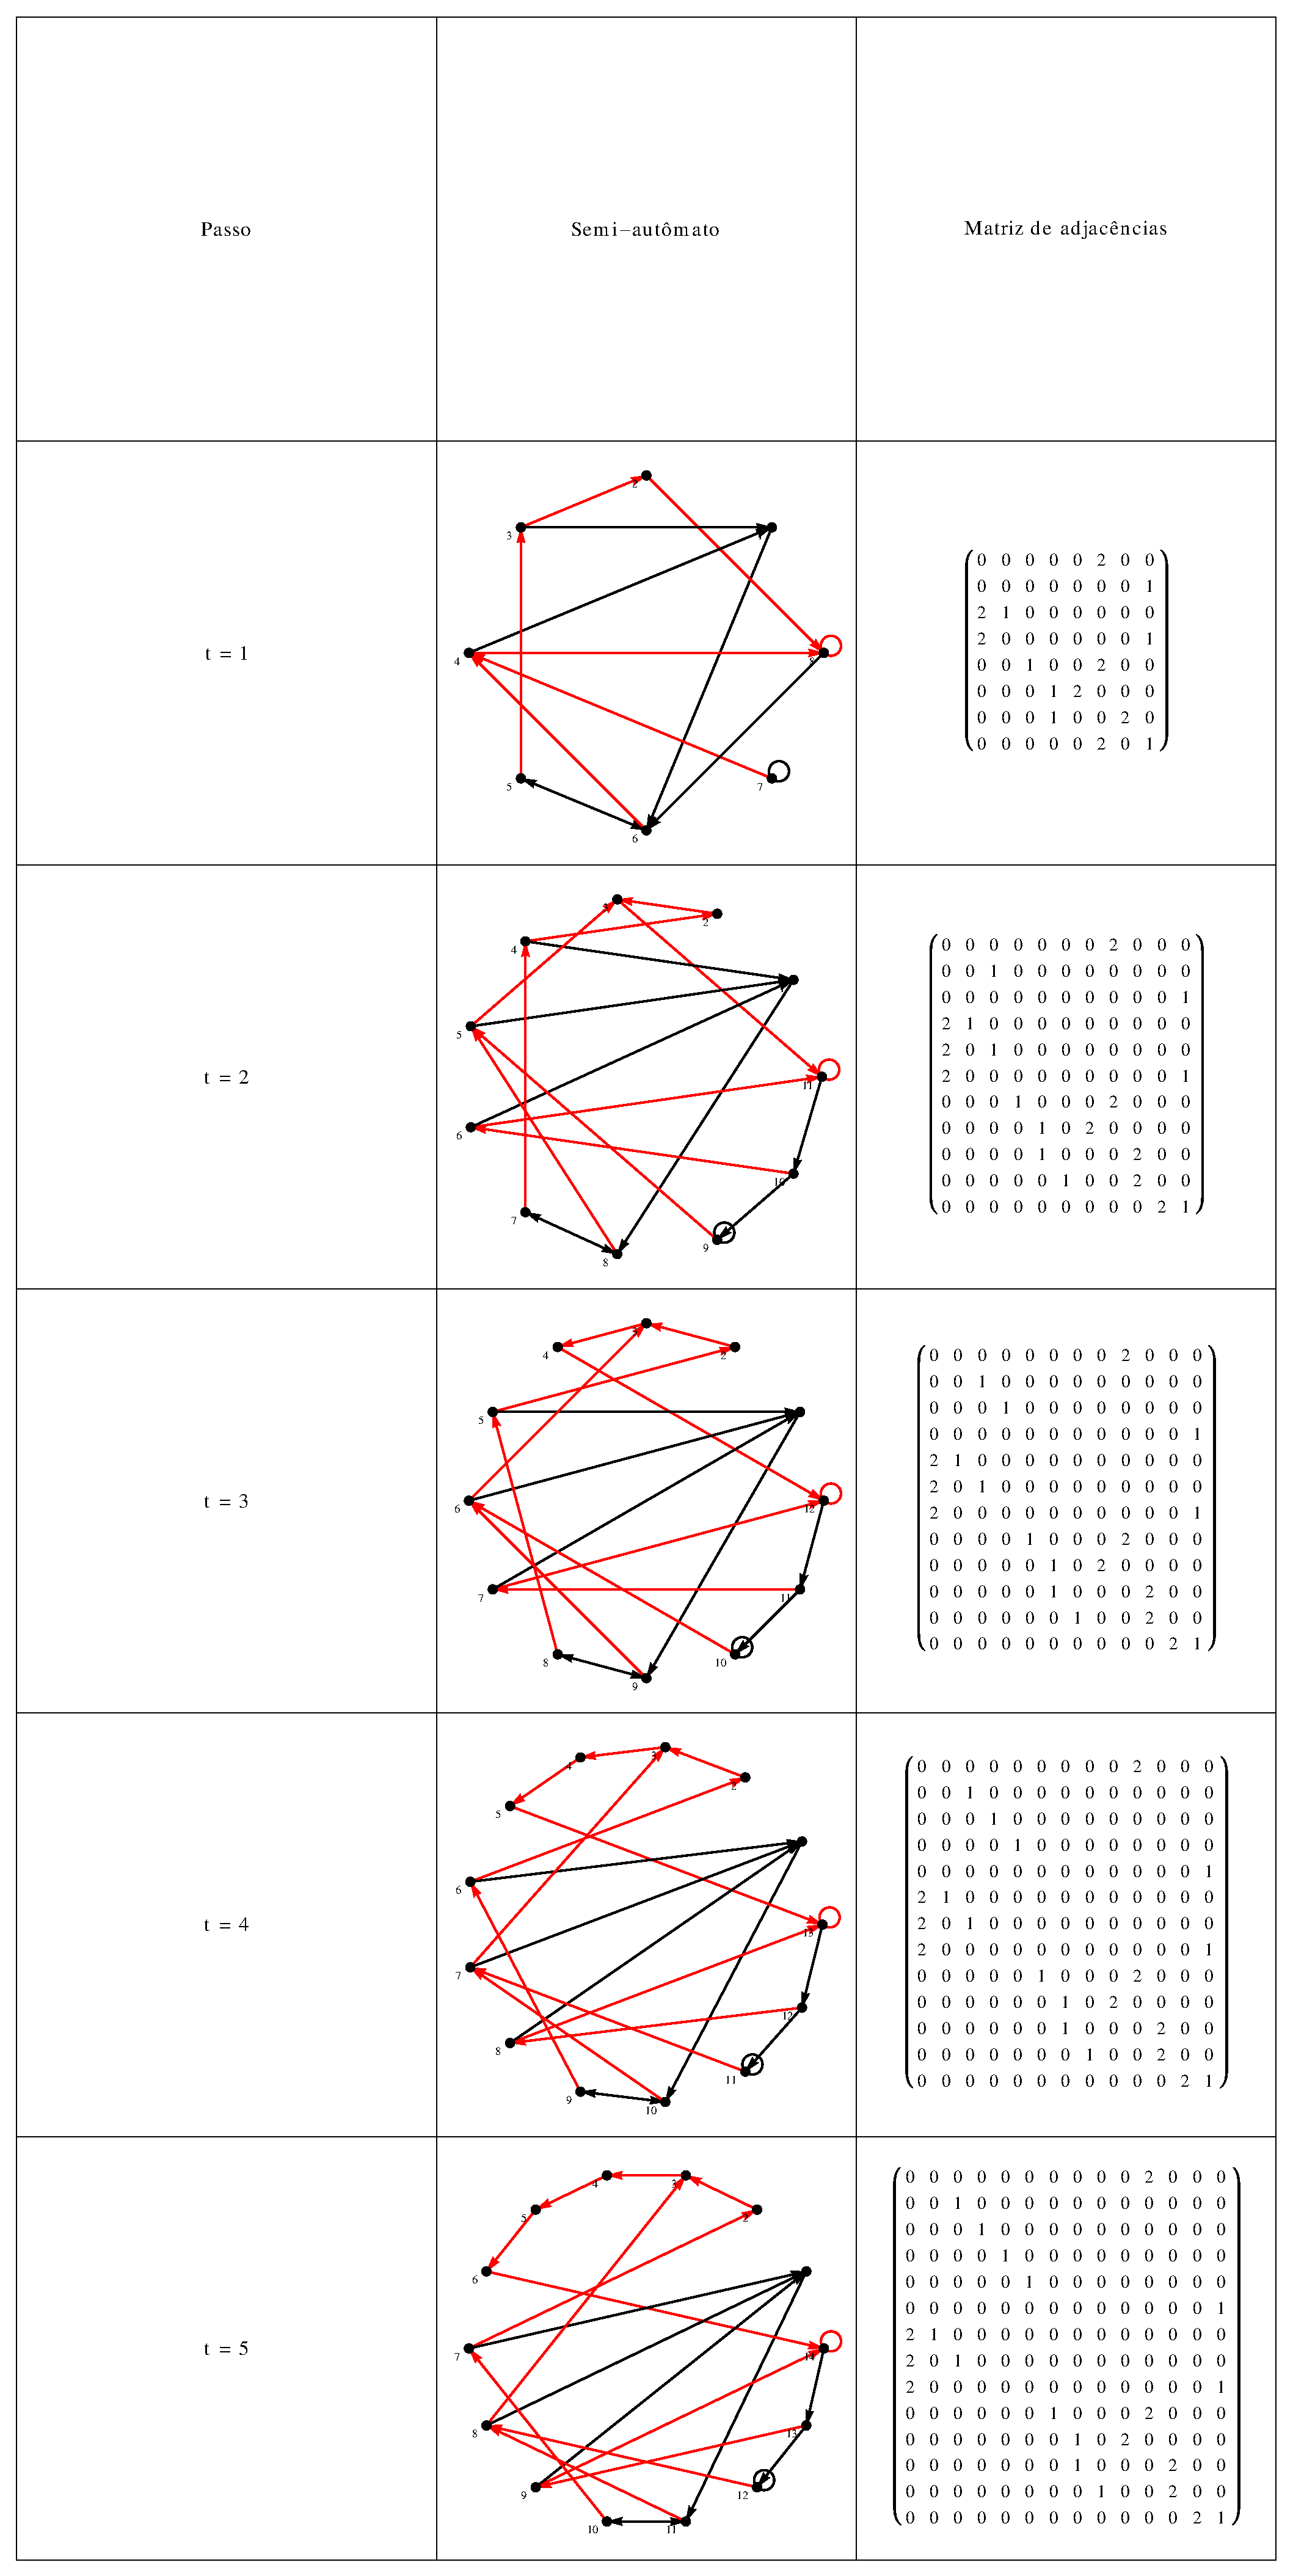
\includegraphics[scale=0.32]{img/mat/matr172.eps}
\caption{Regra 172.}
\label{tab:mr172}
\end{center}
\end{table}

\begin{table}[H]
\begin{center}
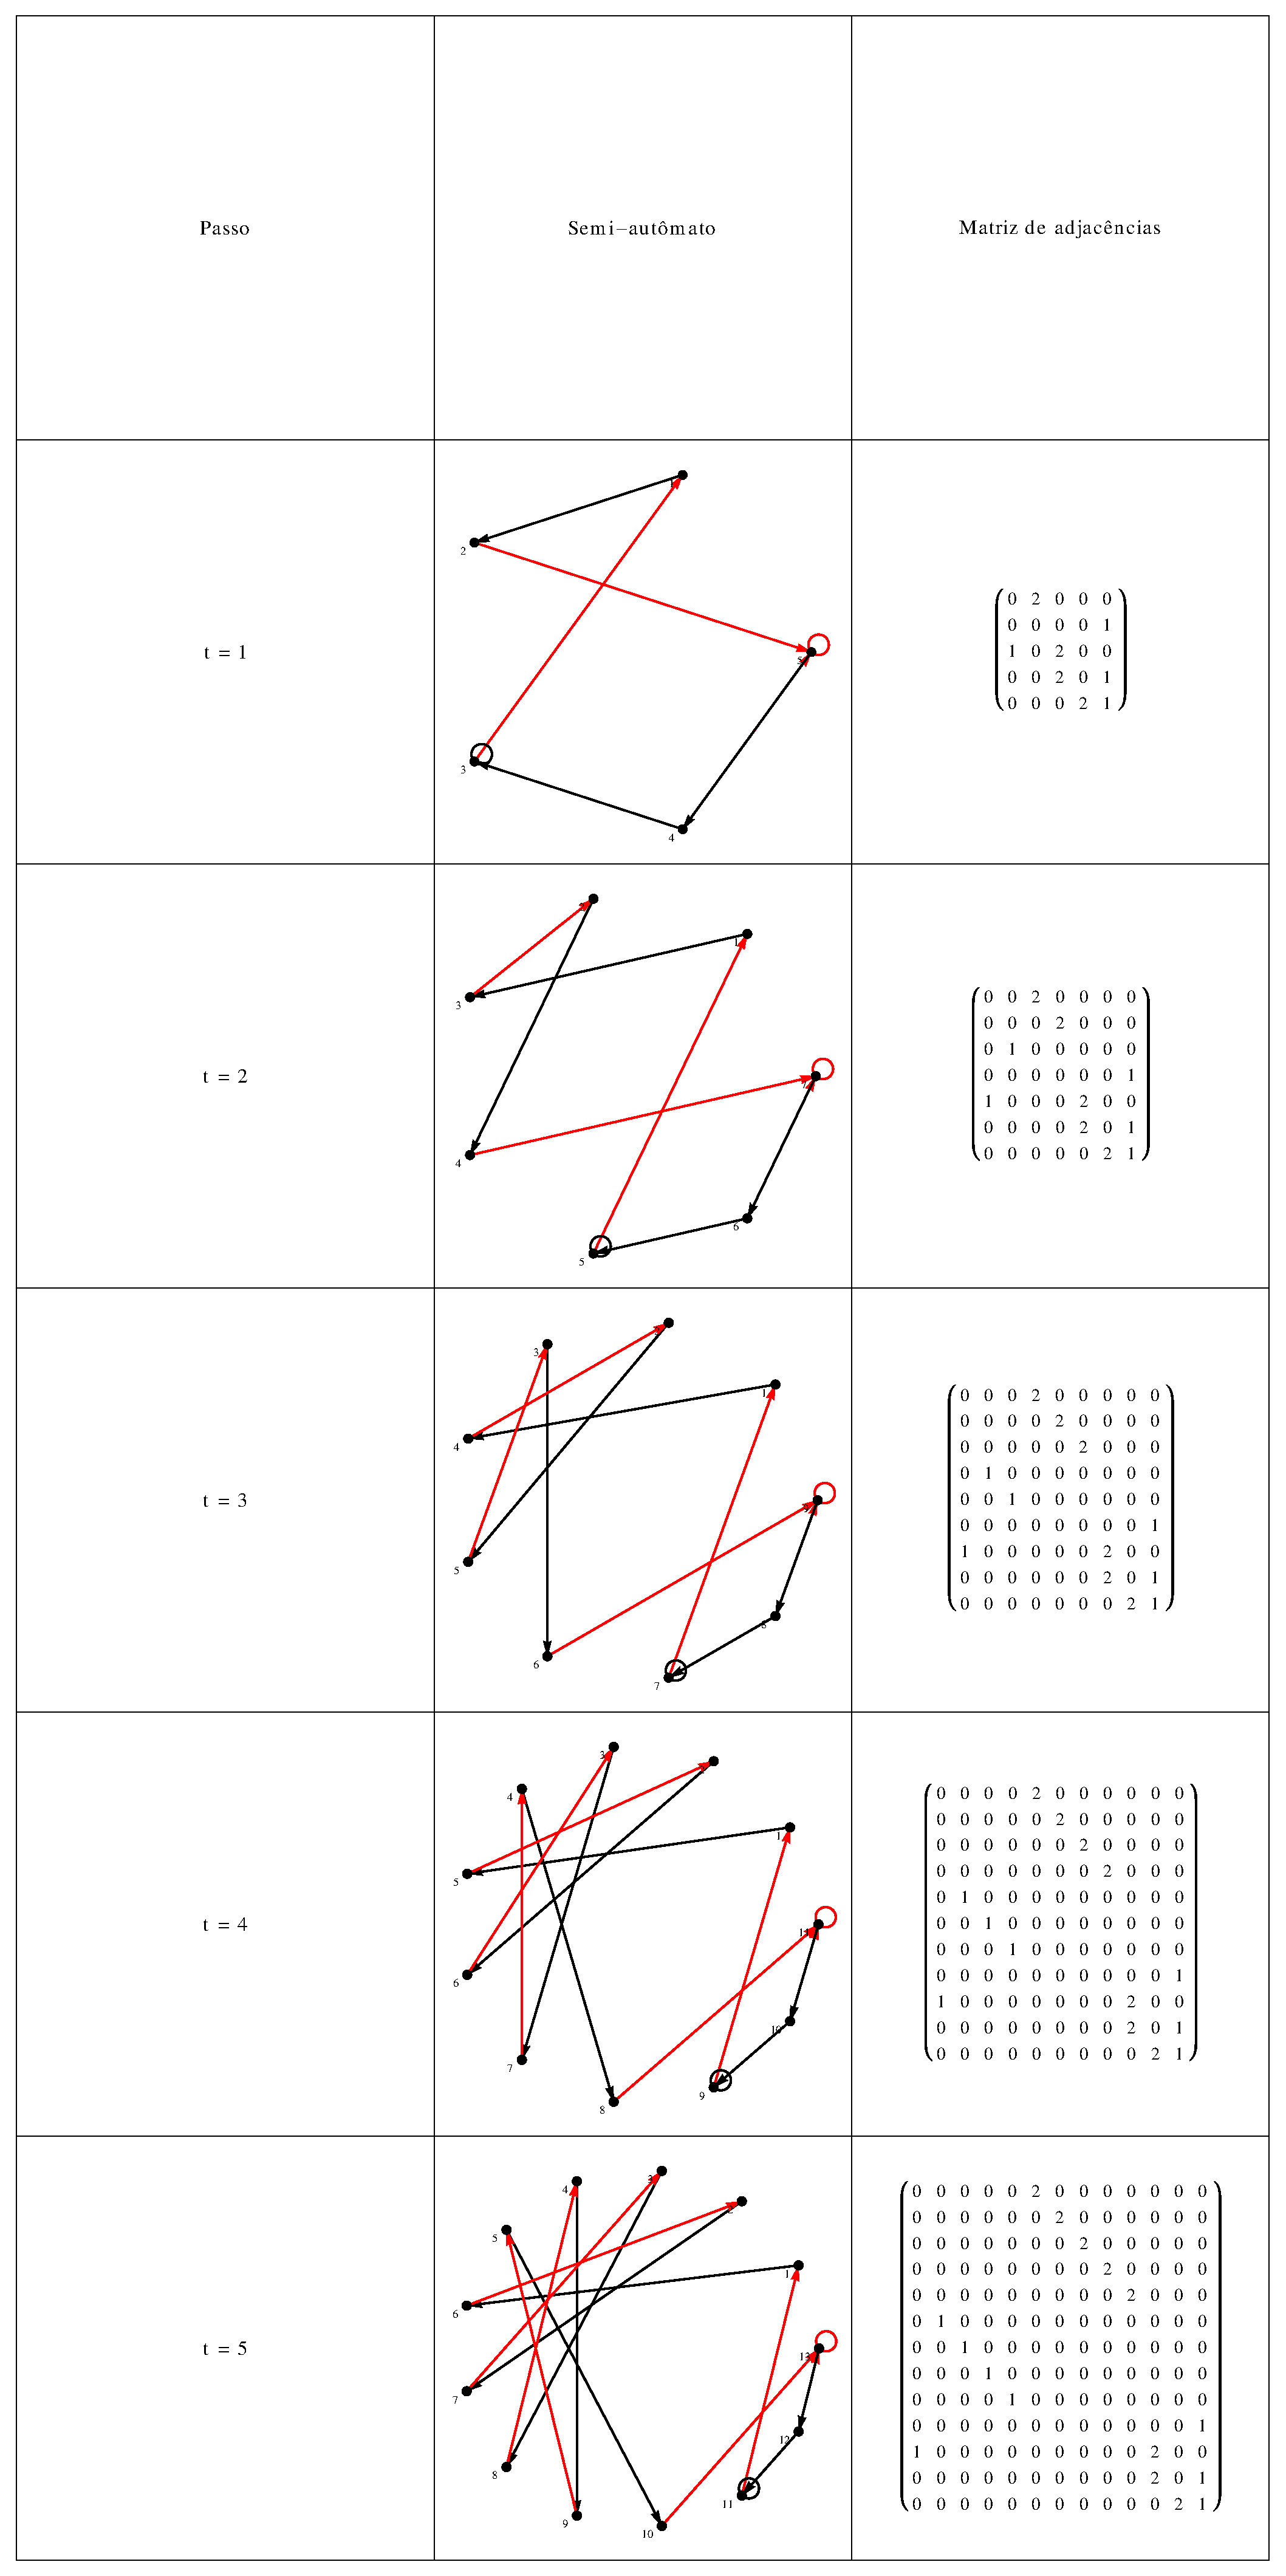
\includegraphics[scale=0.32]{img/mat/matr176.eps}
\caption{Regra 176.}
\label{tab:mr176}
\end{center}
\end{table}

\begin{table}[H]
\begin{center}
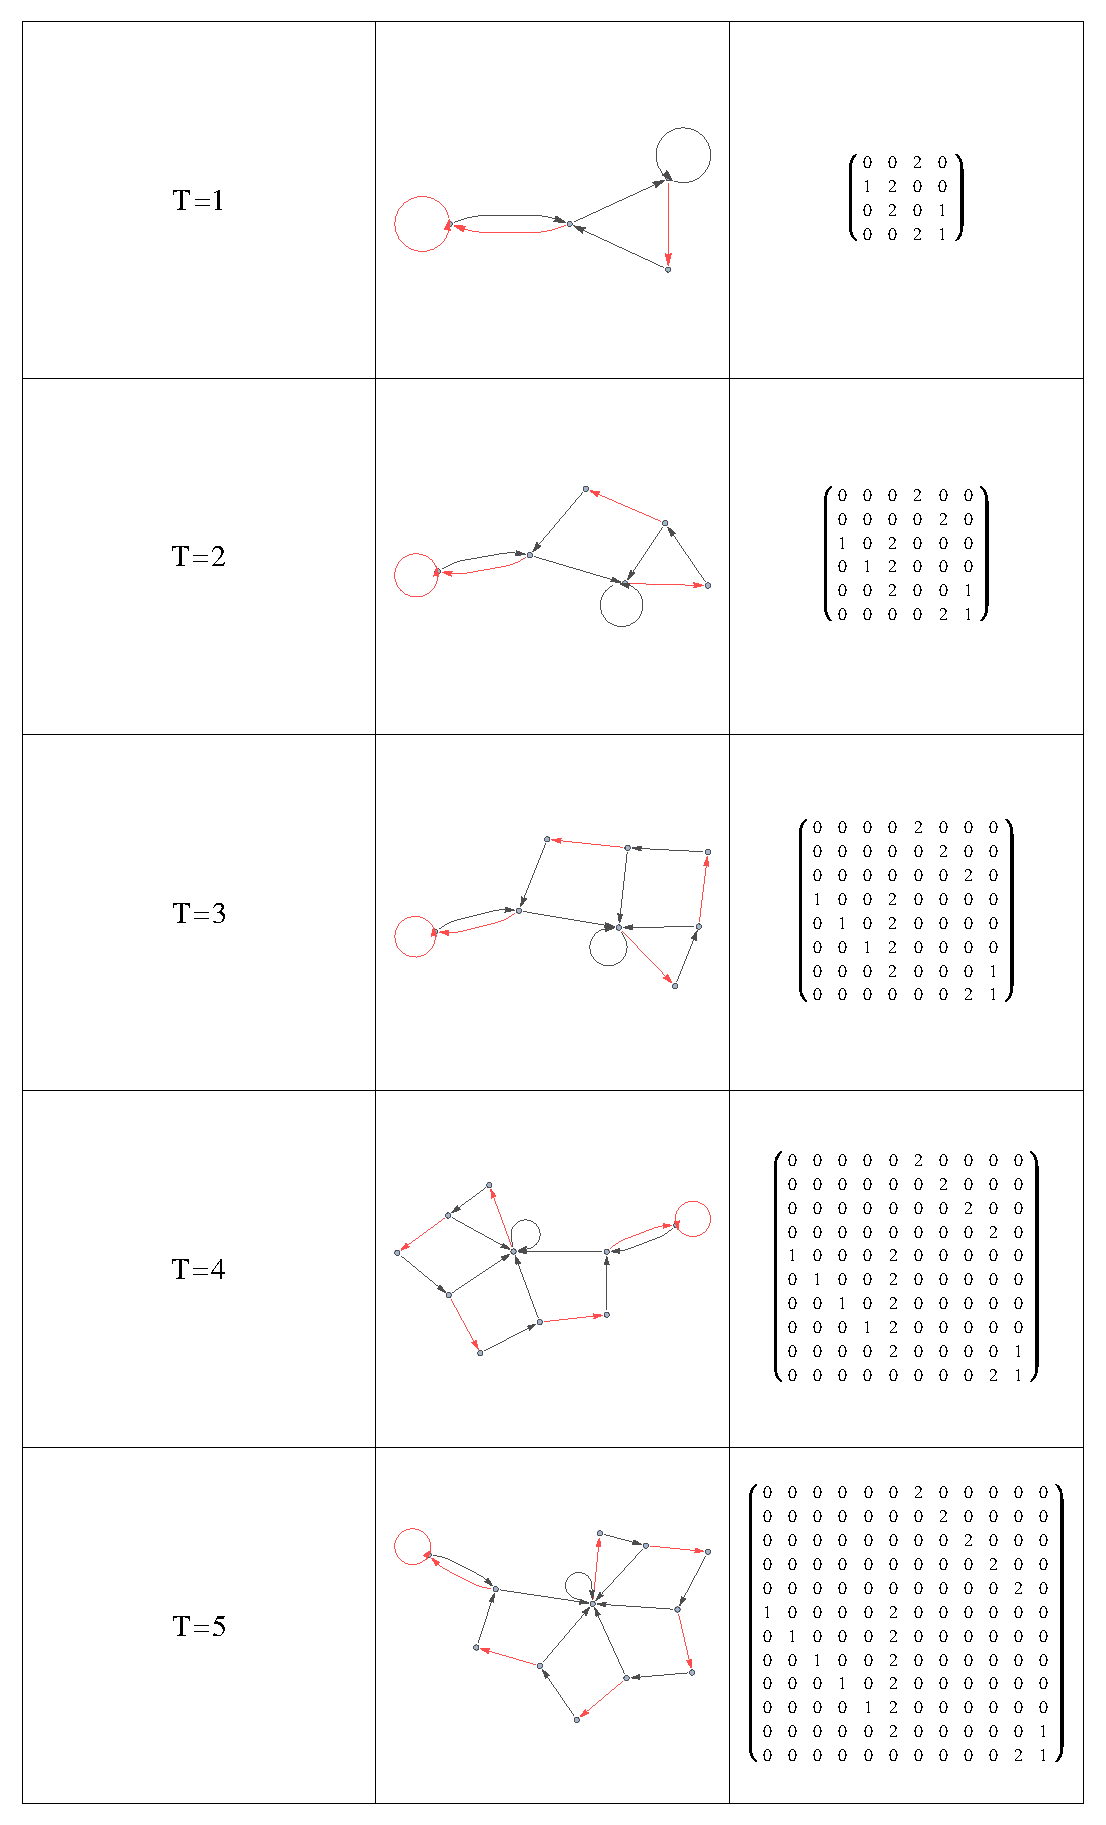
\includegraphics[scale=0.32]{img/mat/matr184.eps}
\caption{Regra 184.}
\label{tab:mr184}
\end{center}
\end{table}

\begin{table}[H]
\begin{center}
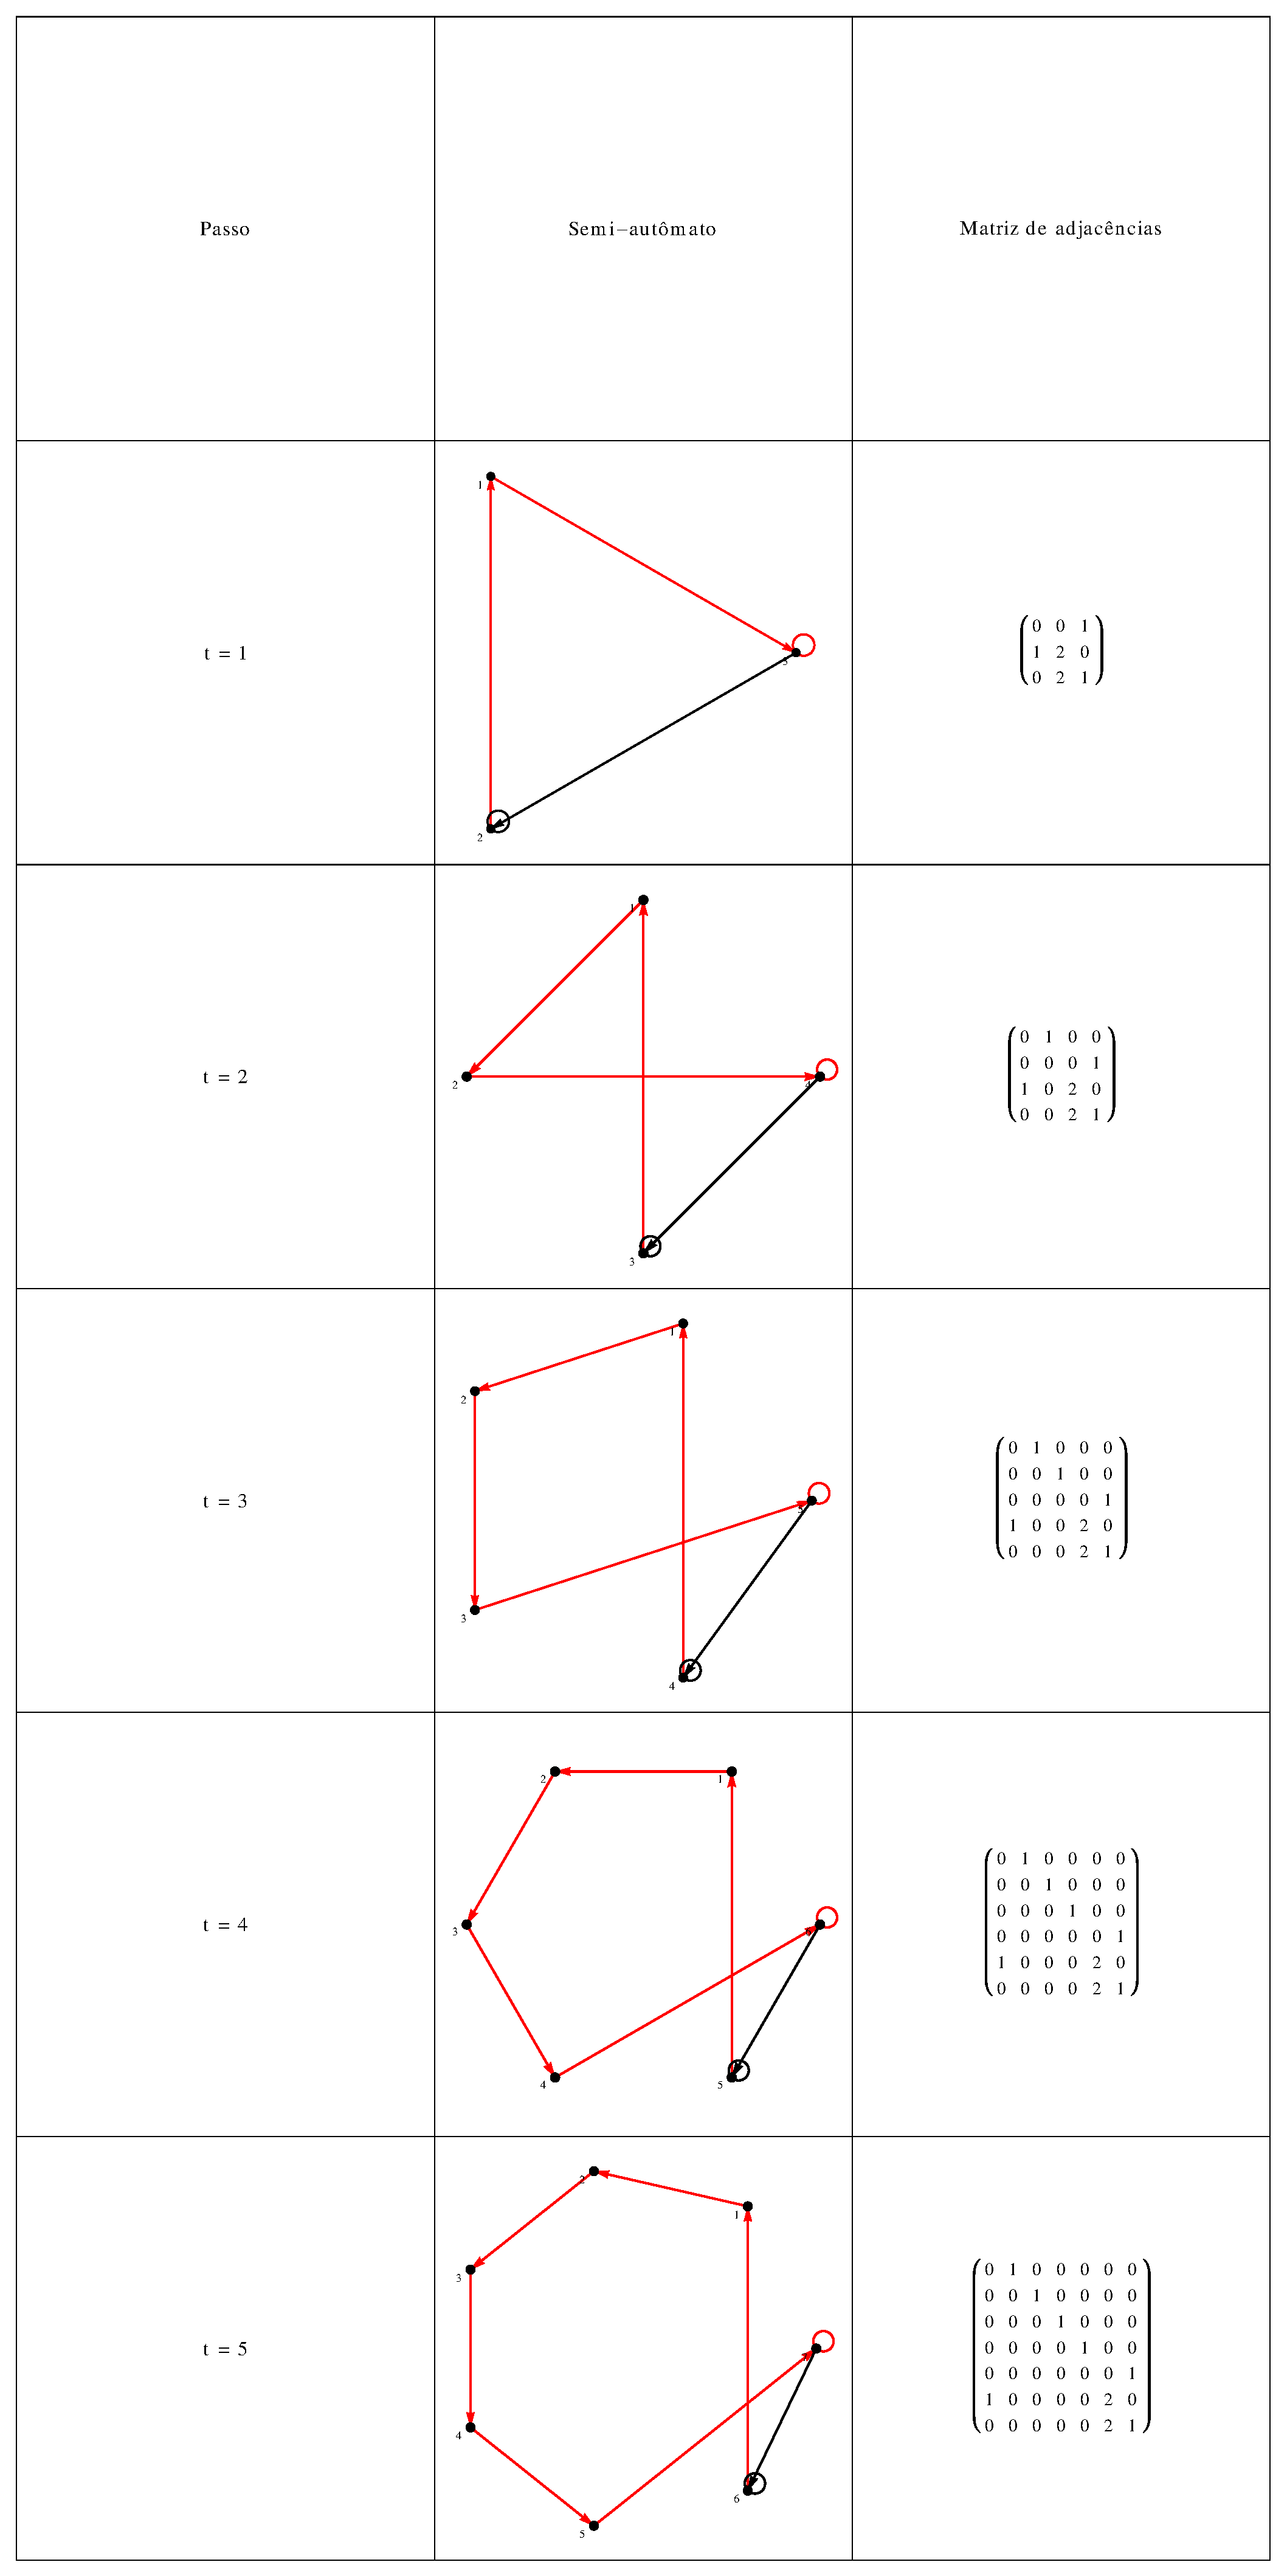
\includegraphics[scale=0.32]{img/mat/matr192.eps}
\caption{Regra 192.}
\label{tab:mr192}
\end{center}
\end{table}

\begin{table}[H]
\begin{center}
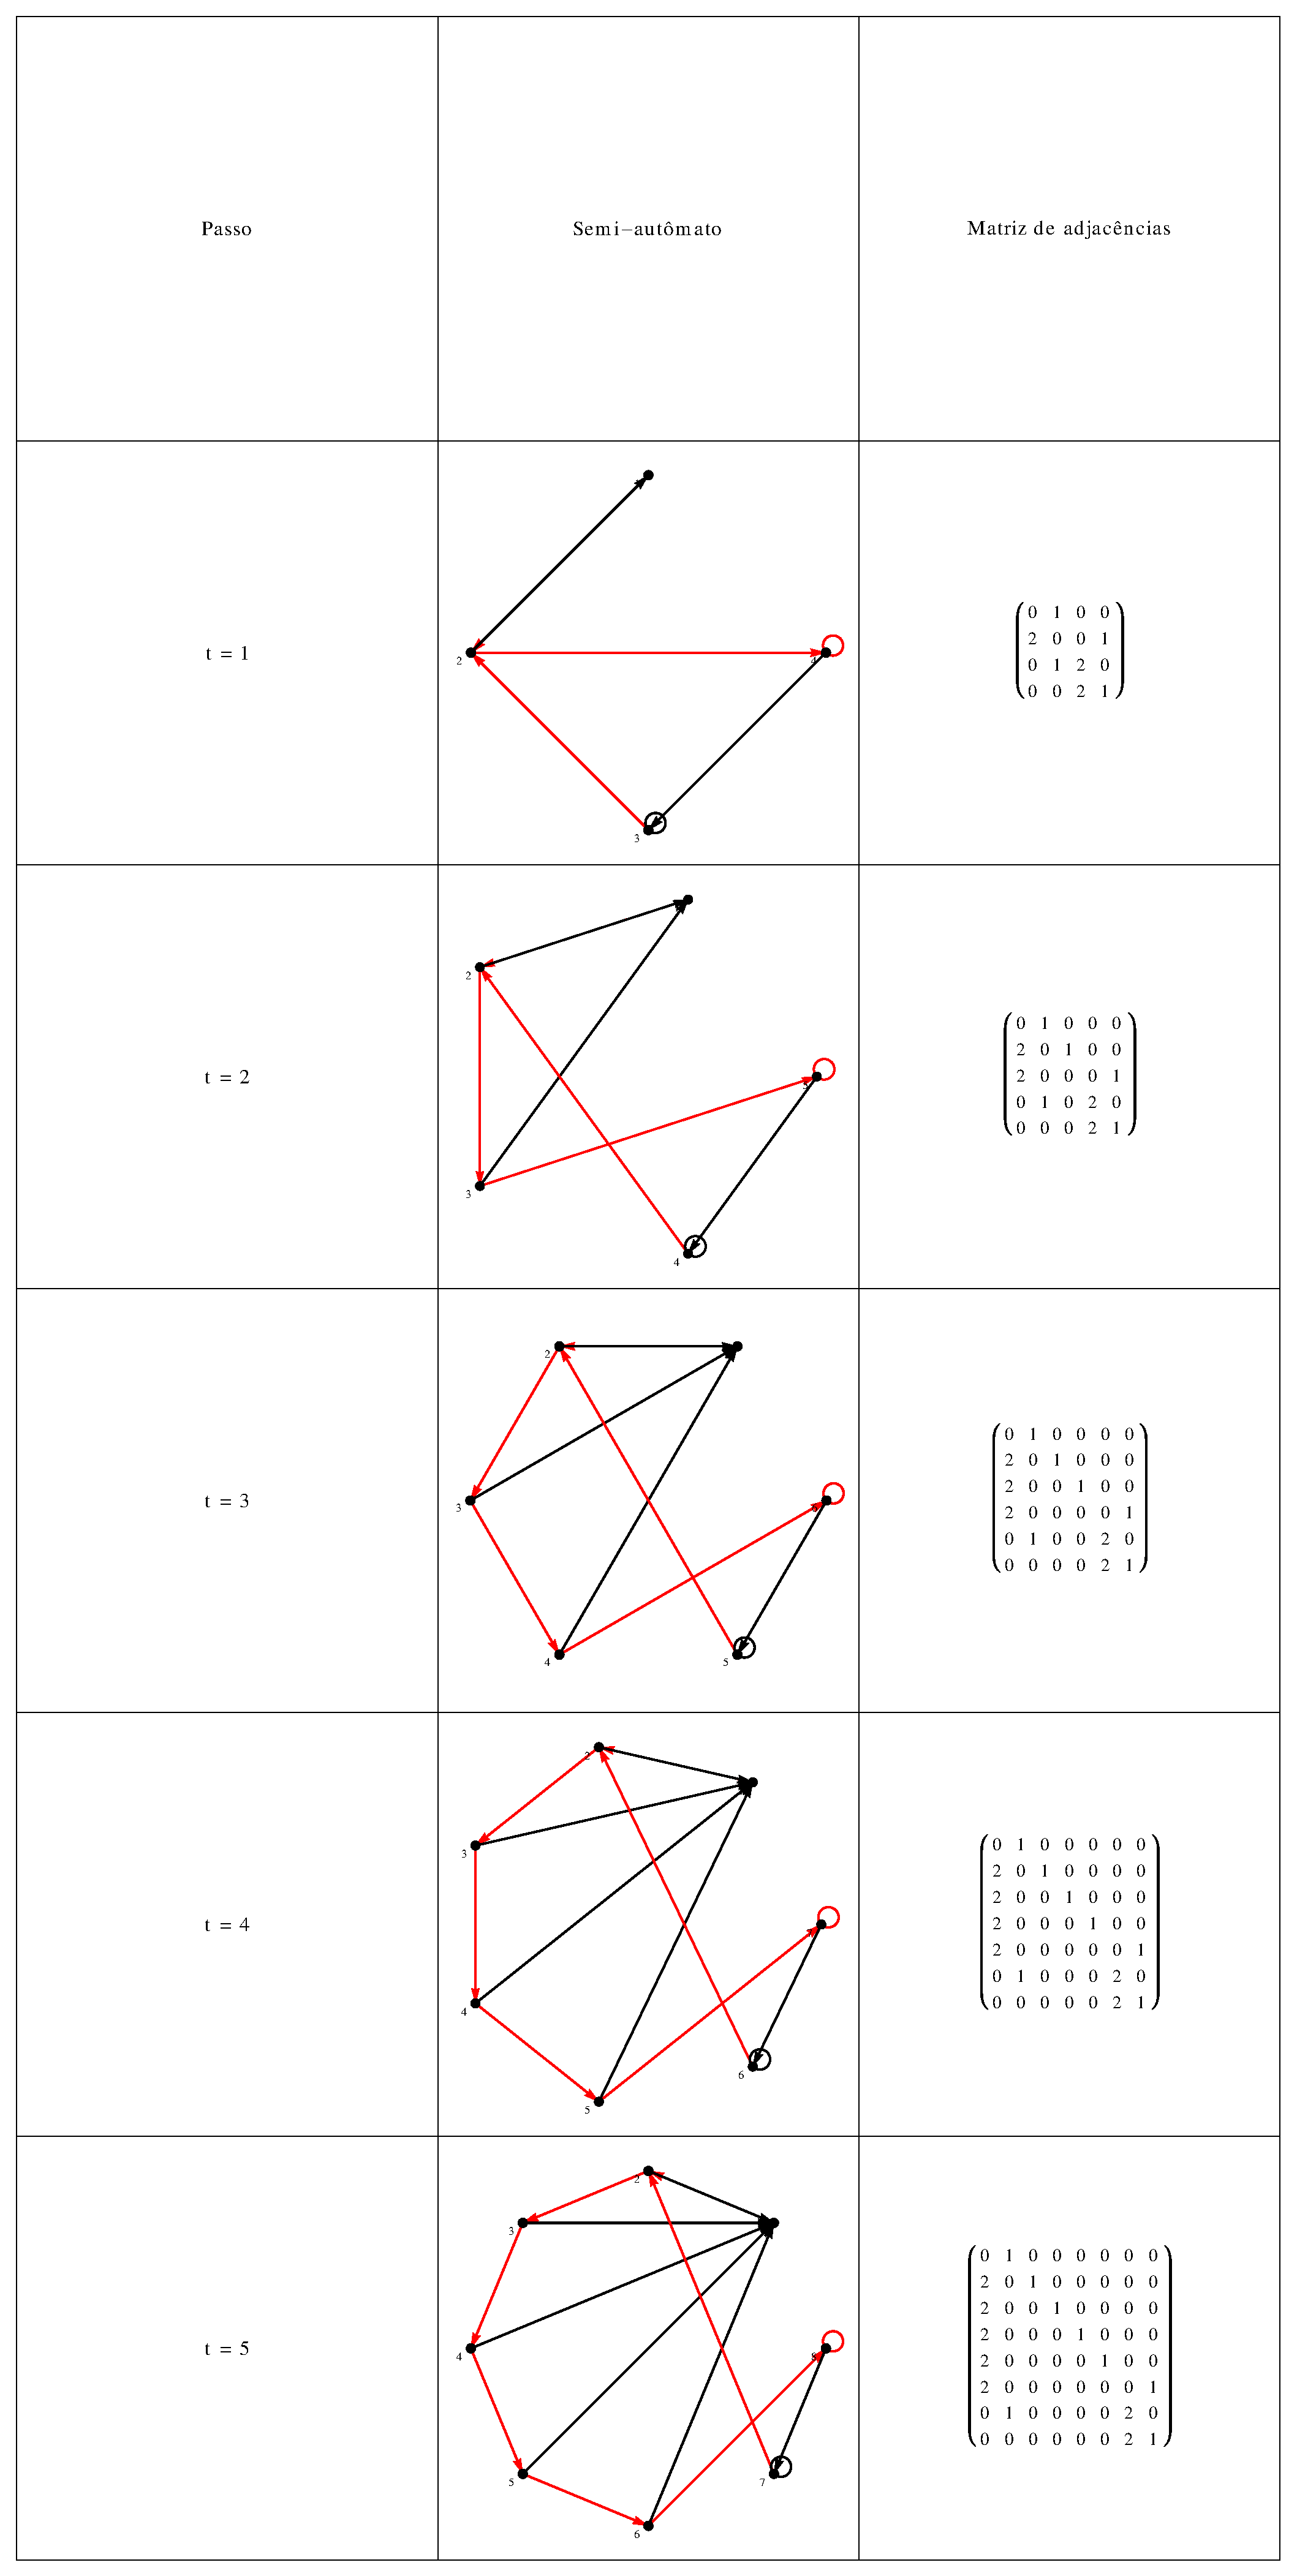
\includegraphics[scale=0.32]{img/mat/matr196.eps}
\caption{Regra 196.}
\label{tab:mr196}
\end{center}
\end{table}

\begin{table}[H]
\begin{center}
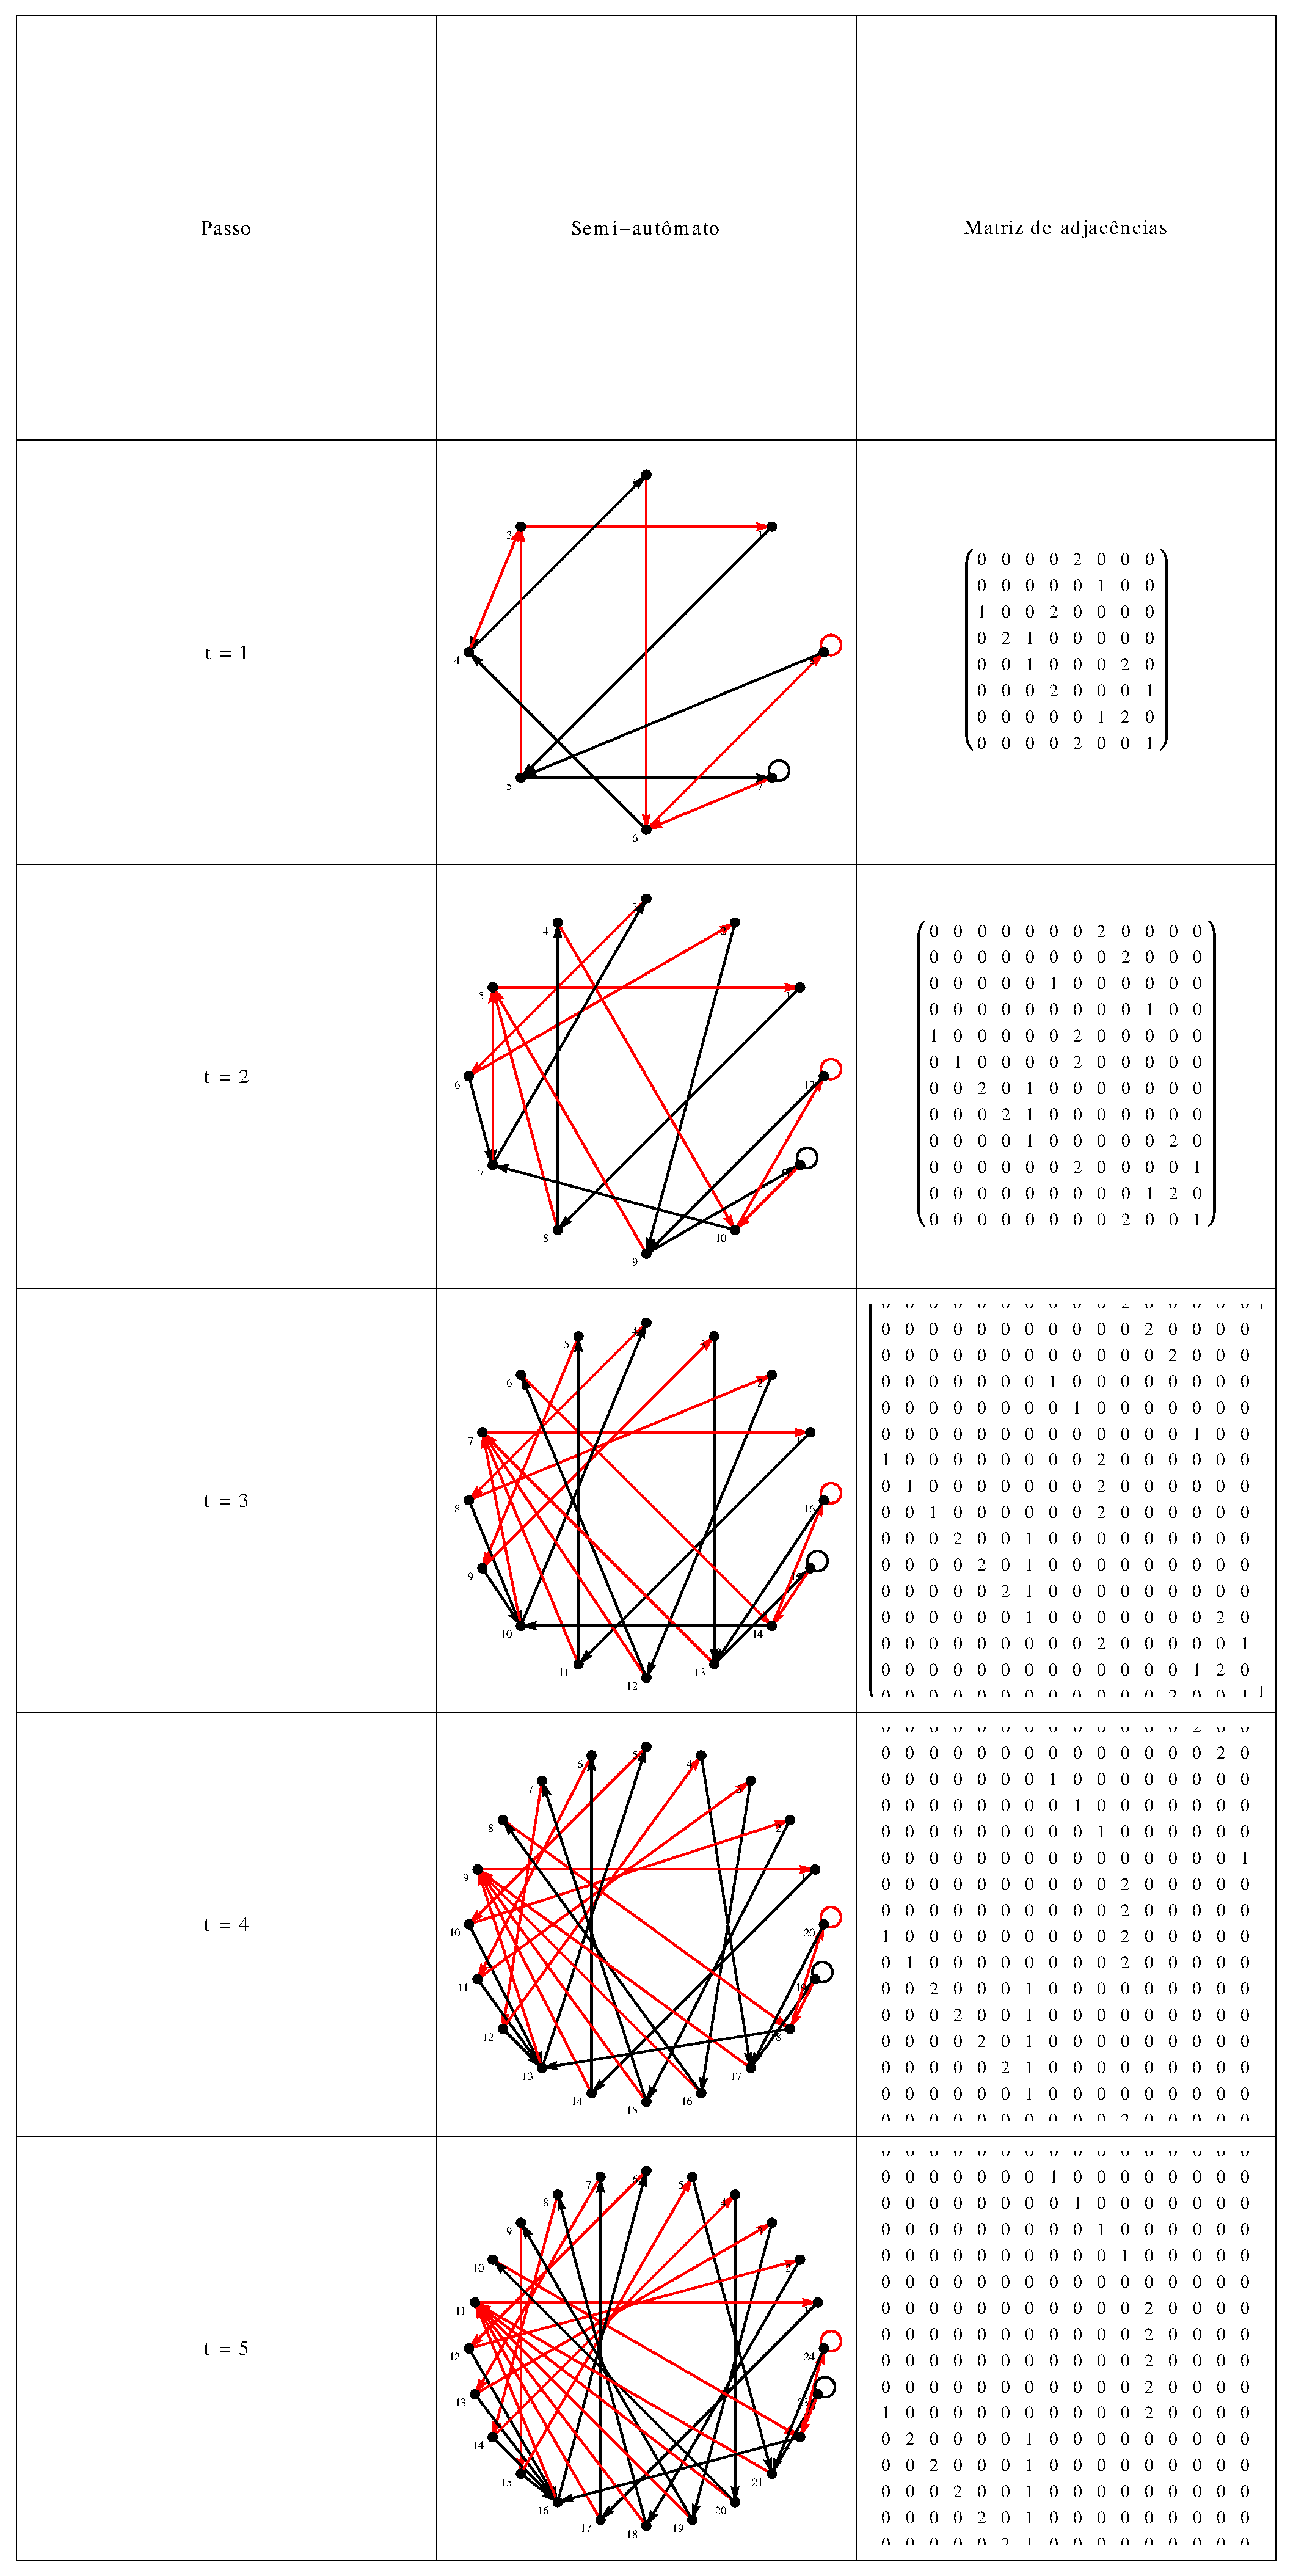
\includegraphics[scale=0.32]{img/mat/matr212.eps}
\caption{Regra 212.}
\label{tab:mr212}
\end{center}
\end{table}

\begin{table}[H]
\begin{center}
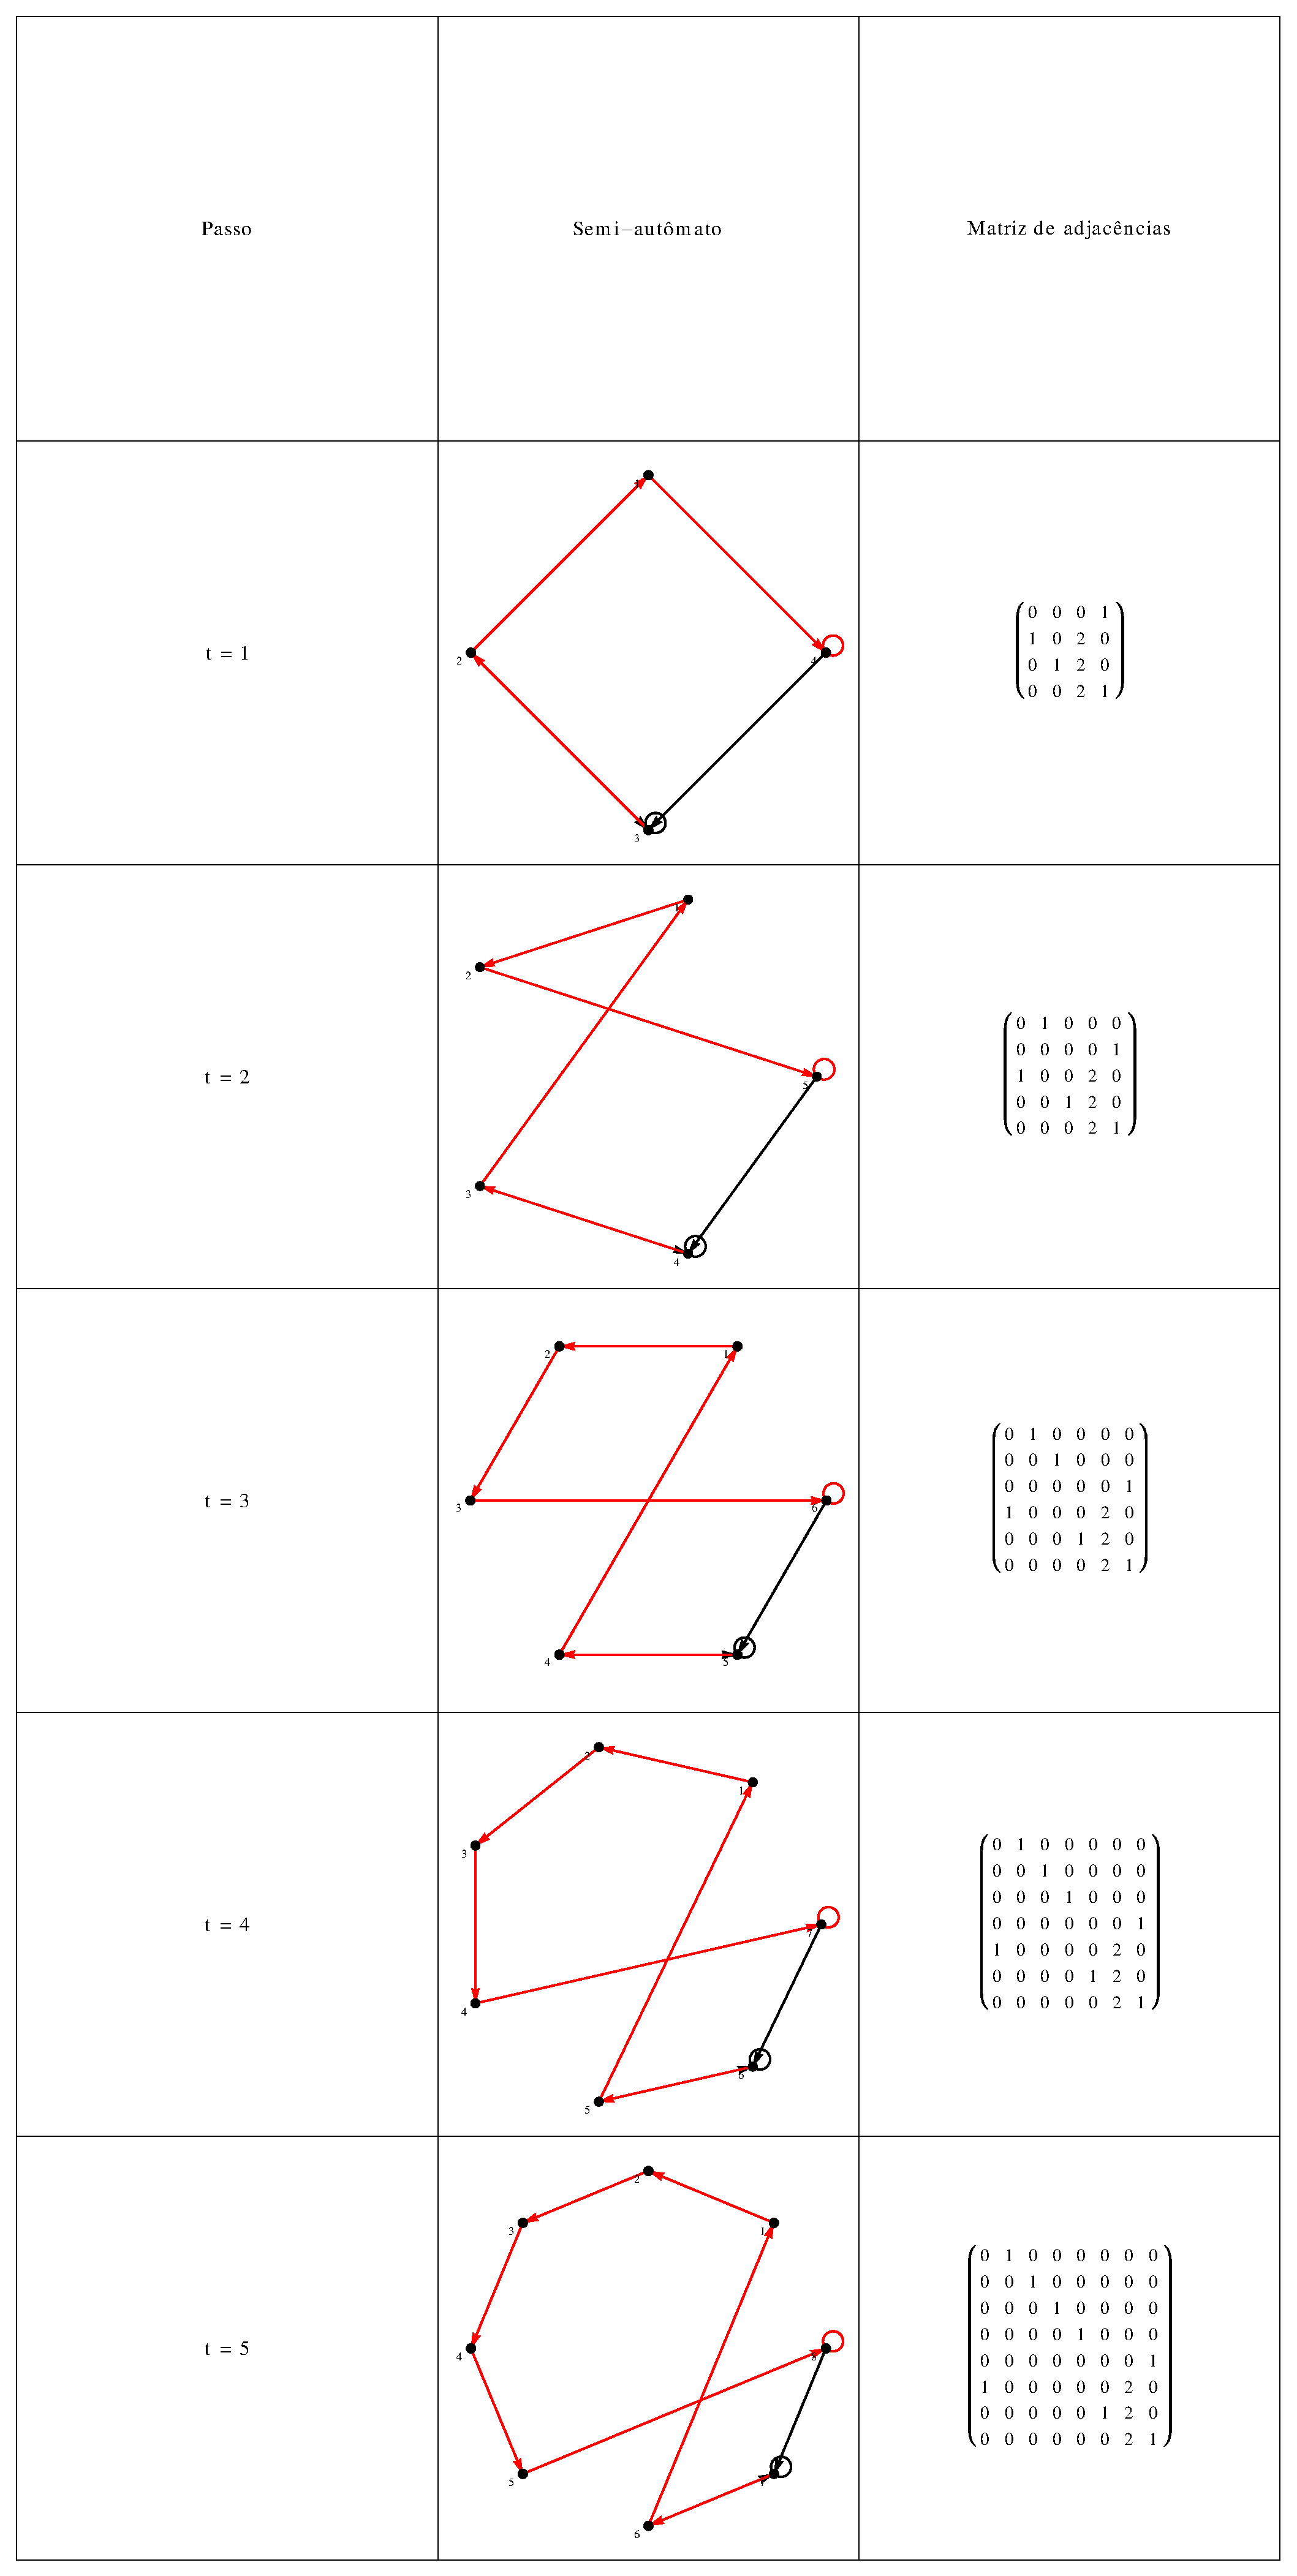
\includegraphics[scale=0.32]{img/mat/matr224.eps}
\caption{Regra 224.}
\label{tab:mr224}
\end{center}
\end{table}

\begin{table}[H]
\begin{center}
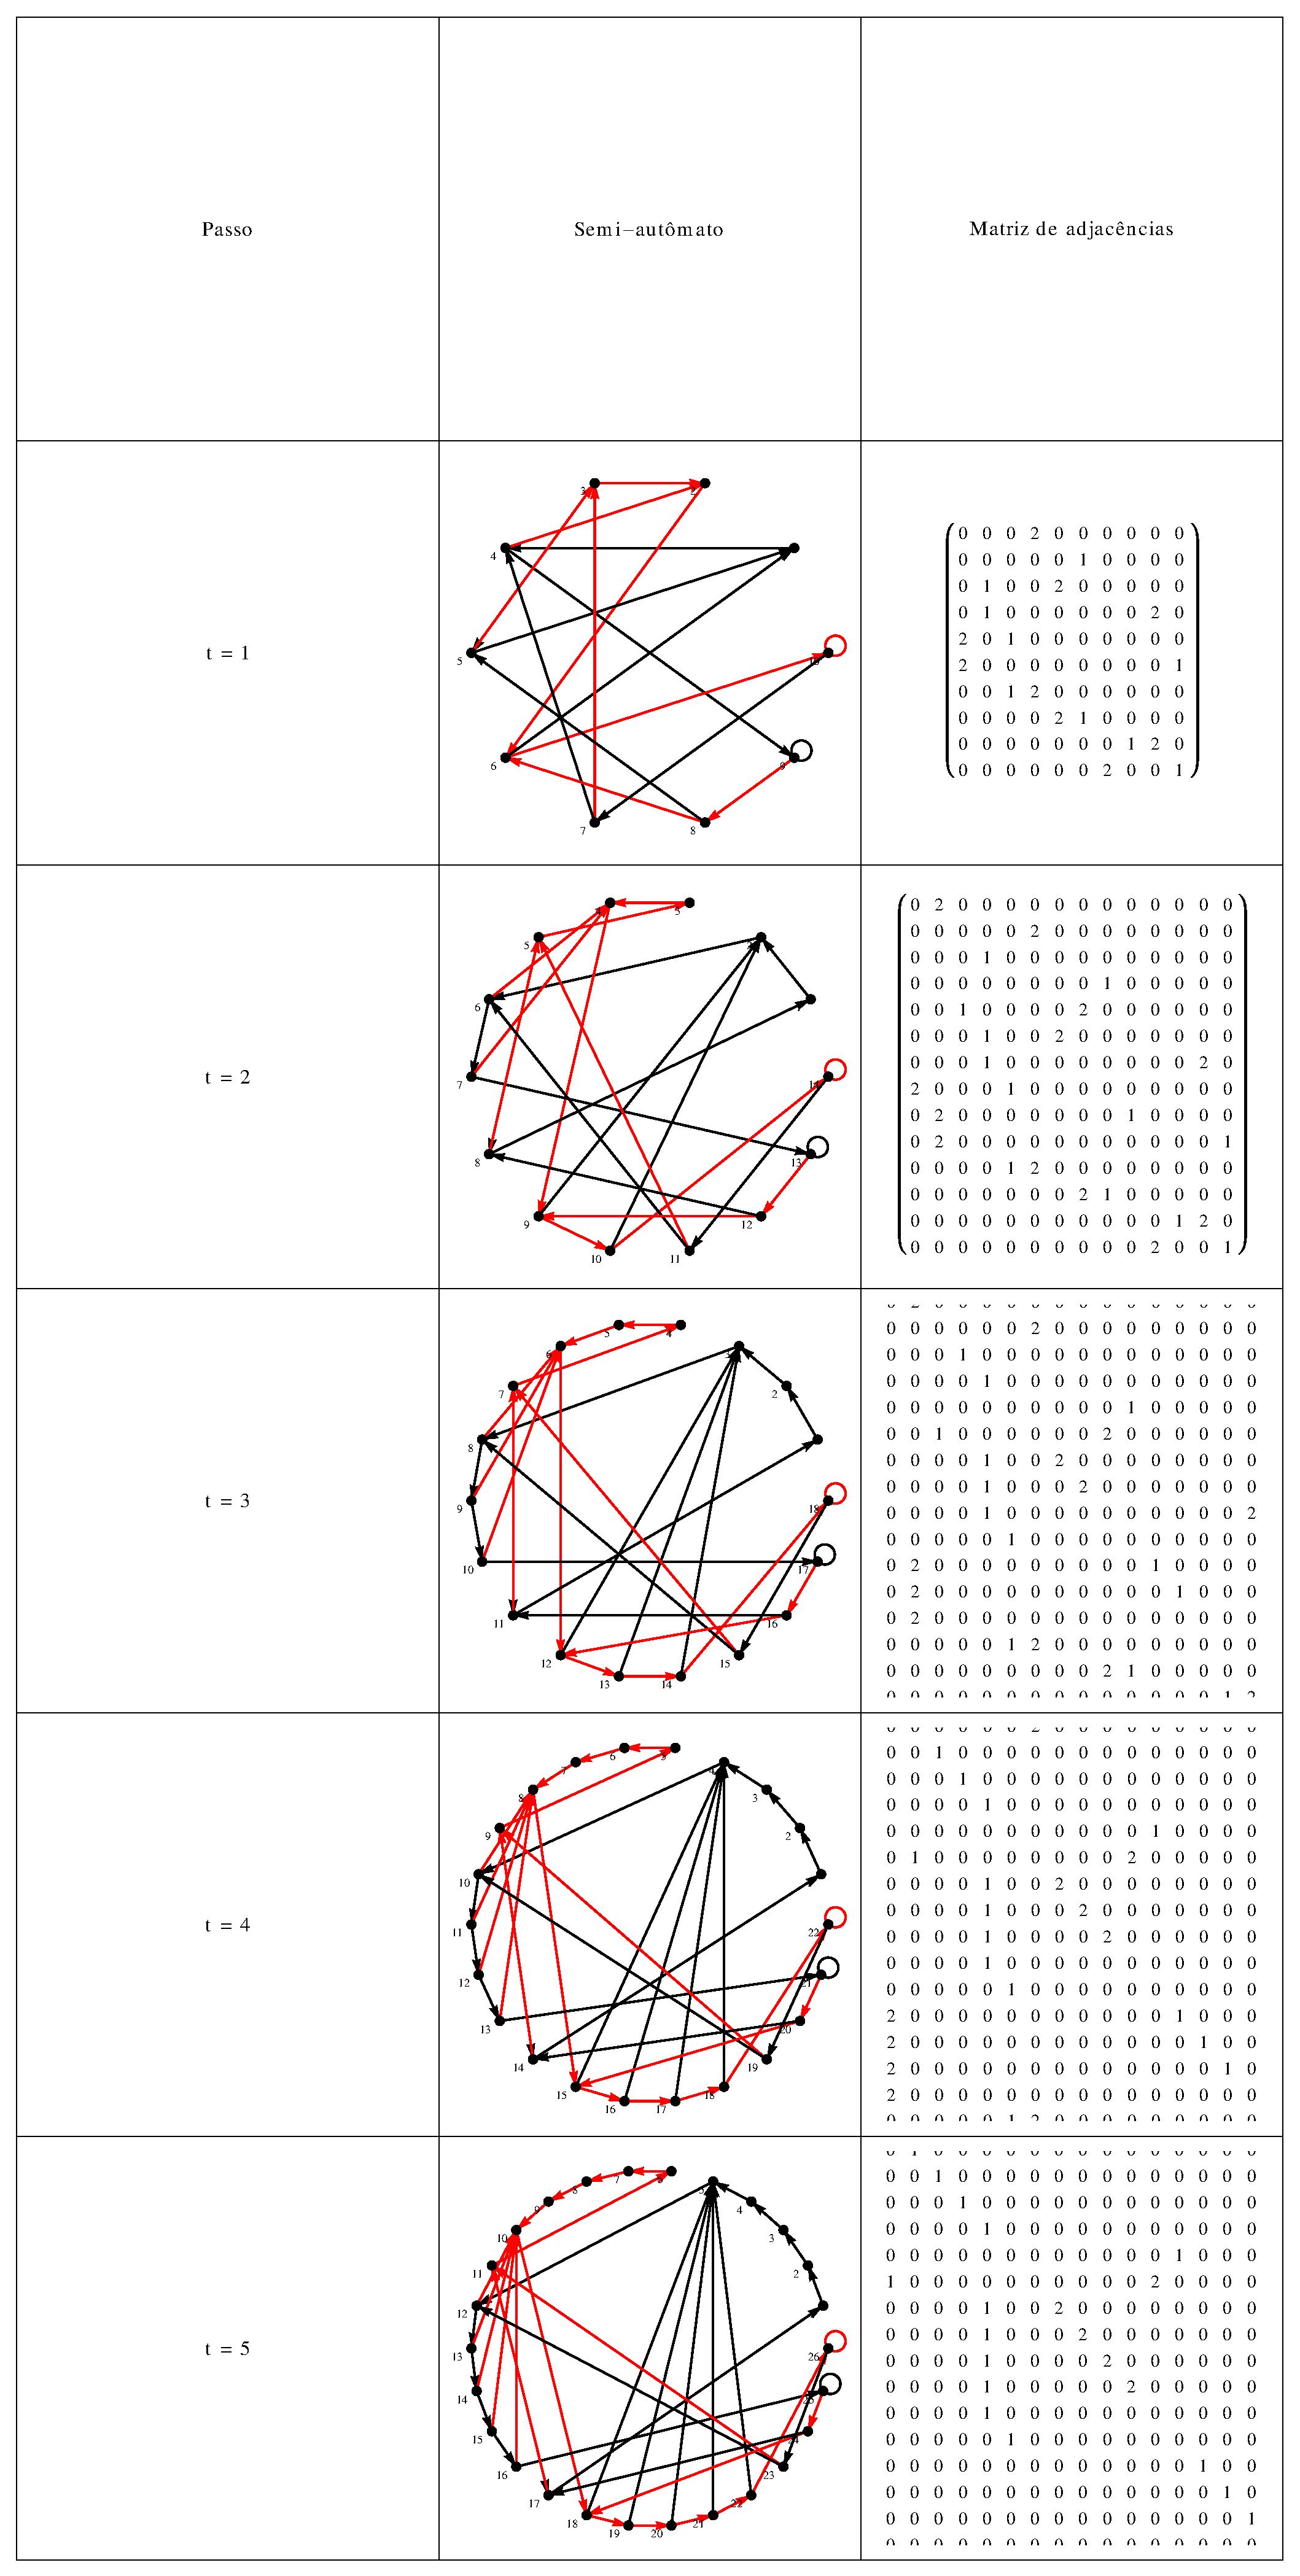
\includegraphics[scale=0.32]{img/mat/matr232.eps}
\caption{Regra 232.}
\label{tab:mr232}
\end{center}
\end{table}

\def\refname{Referências Bibliográficas}
\bibliography{masterthesis}
\addcontentsline{toc}{section}{REFERÊNCIAS BIBLIOGRÁFICAS} 
\bibliographystyle{abnt-alf}

\end{document}

% vim:set spell spelllang=pt
